\chapter{Aspectos teóricos y revisión de la literatura}

En esta sección se abarcan los aspectos relacionados al conocimiento general para la comprensión del presente trabajo (aspectos teóricos) y la revisión de la literatura asociada al trabajo presentado en esta tesis. %Para realizar un análisis de la Programación Genética aplicada a problemas NP-Hard es necesario conocer la base teórica de ésta. Para ello, se exponen los conceptos fundamentales de la computación evolutiva y la Programación Genética. La sección 2.1 se centra en explicar aquellas partes fundamentales al tema que se trata en esta tesis. De la revisión de la literatura se desprende lo presentado en la sección 2.2.

%%%%%%%%%%%%% IDEA %%%%%%%%%%%%%%%%%%%%%%%%%%%%%%%%%%%%
% Un párrafo para comparar los problemas conejillos de india con los que se compara. Para evaluar el desempeño de los algoritmos tipicamente se usan problemas problemas de aprendizaje de la literatura.
%%%%%%%%%%%%%%%%%%%%%%%%%%%%%%%%%%%%%%%%%%%%%%%%%%%%%


%%%%%%%%%%%%% IDEA %%%%%%%%%%%%%%%%%%%%%%%%%%%%%%%%%%%%
% Las características del SGD y el problema del desvanecimiento. Las heurísticas y metaheurísticas.
%%%%%%%%%%%%%%%%%%%%%%%%%%%%%%%%%%%%%%%%%%%%%%%%%%%%%

\section{Aspectos teóricos}
\subsection{Redes neuronales multicapas}
Una de las características que diferencia a las neuronas biológicas del resto de las células vivas, es su capacidad de comunicación. En la figura \ref{fig:neurona} se puede apreciar un esquema general de una neurona biológica. Las dendritas y el soma (cuerpo celular) reciben las señales de entrada; el cuerpo celular las combina e integra y emite una señal de salida. El axón transporta esas señales a los terminales axónicos, que se encargan de distribuir información a un nuevo conjunto de neuronas. Por lo general, una neurona recibe información de miles de otras neuronas, y a su vez, envía información a otras neuronas, formando una red de conexiones.
\begin{imagen}
	\scalebox{0.07}{
\definecolor{ca2a0a1}{RGB}{162,160,161}
\definecolor{c424142}{RGB}{66,65,66}


\begin{tikzpicture}[y=0.80pt, x=0.80pt, yscale=-1.000000, xscale=1.000000, inner sep=0pt, outer sep=0pt]
\begin{scope}[shift={(-21.2132,-191.88818)},fill=ca2a0a1]
  \path[fill] (460.0000,1758.0000) .. controls (460.0000,1729.0000) and
    (465.0000,1698.0000) .. (470.0000,1690.0000) .. controls (477.0000,1679.0000)
    and (480.0000,1695.0000) .. (480.0000,1743.0000) .. controls
    (480.0000,1781.0000) and (476.0000,1810.0000) .. (470.0000,1810.0000) ..
    controls (465.0000,1810.0000) and (460.0000,1786.0000) .. (460.0000,1758.0000)
    -- cycle;
  \path[fill] (405.0000,1790.0000) .. controls (401.0000,1784.0000) and
    (406.0000,1783.0000) .. (416.0000,1787.0000) .. controls (429.0000,1792.0000)
    and (431.0000,1790.0000) .. (425.0000,1780.0000) .. controls
    (420.0000,1771.0000) and (421.0000,1769.0000) .. (429.0000,1774.0000) ..
    controls (435.0000,1778.0000) and (438.0000,1786.0000) .. (435.0000,1791.0000)
    .. controls (427.0000,1803.0000) and (413.0000,1803.0000) ..
    (405.0000,1790.0000) -- cycle;
  \path[fill] (390.0000,1749.0000) .. controls (390.0000,1744.0000) and
    (395.0000,1742.0000) .. (400.0000,1745.0000) .. controls (406.0000,1748.0000)
    and (410.0000,1753.0000) .. (410.0000,1756.0000) .. controls
    (410.0000,1758.0000) and (406.0000,1760.0000) .. (400.0000,1760.0000) ..
    controls (395.0000,1760.0000) and (390.0000,1755.0000) .. (390.0000,1749.0000)
    -- cycle;
  \path[fill] (423.0000,1753.0000) .. controls (427.0000,1750.0000) and
    (433.0000,1750.0000) .. (437.0000,1753.0000) .. controls (440.0000,1757.0000)
    and (437.0000,1760.0000) .. (430.0000,1760.0000) .. controls
    (423.0000,1760.0000) and (420.0000,1757.0000) .. (423.0000,1753.0000) --
    cycle;
  \path[fill] (364.0000,1728.0000) .. controls (360.0000,1721.0000) and
    (361.0000,1720.0000) .. (368.0000,1724.0000) .. controls (380.0000,1731.0000)
    and (384.0000,1740.0000) .. (376.0000,1740.0000) .. controls
    (373.0000,1740.0000) and (368.0000,1735.0000) .. (364.0000,1728.0000) --
    cycle;
  \path[fill] (406.0000,1725.0000) .. controls (403.0000,1717.0000) and
    (405.0000,1710.0000) .. (410.0000,1710.0000) .. controls (416.0000,1710.0000)
    and (420.0000,1717.0000) .. (420.0000,1725.0000) .. controls
    (420.0000,1733.0000) and (418.0000,1740.0000) .. (416.0000,1740.0000) ..
    controls (414.0000,1740.0000) and (410.0000,1733.0000) .. (406.0000,1725.0000)
    -- cycle;

  \path[fill] (1162.0000,1724.0000) .. controls (1155.0000,1716.0000) and
    (1154.0000,1710.0000) .. (1159.0000,1710.0000) .. controls
    (1169.0000,1710.0000) and (1184.0000,1729.0000) .. (1179.0000,1735.0000) ..
    controls (1177.0000,1736.0000) and (1169.0000,1732.0000) ..
    (1162.0000,1724.0000) -- cycle;
  \path[fill] (317.0000,1708.0000) .. controls (321.0000,1689.0000) and
    (320.0000,1688.0000) .. (310.0000,1700.0000) .. controls (302.0000,1710.0000)
    and (300.0000,1711.0000) .. (302.0000,1702.0000) .. controls
    (304.0000,1694.0000) and (309.0000,1689.0000) .. (313.0000,1689.0000) ..
    controls (322.0000,1690.0000) and (380.0000,1626.0000) .. (380.0000,1615.0000)
    .. controls (380.0000,1611.0000) and (372.0000,1611.0000) ..
    (363.0000,1614.0000) .. controls (353.0000,1618.0000) and (349.0000,1618.0000)
    .. (353.0000,1614.0000) .. controls (357.0000,1610.0000) and
    (347.0000,1601.0000) .. (330.0000,1594.0000) .. controls (308.0000,1584.0000)
    and (300.0000,1574.0000) .. (300.0000,1555.0000) .. controls
    (300.0000,1541.0000) and (305.0000,1530.0000) .. (311.0000,1530.0000) ..
    controls (318.0000,1530.0000) and (320.0000,1540.0000) .. (316.0000,1556.0000)
    .. controls (310.0000,1578.0000) and (312.0000,1581.0000) ..
    (325.0000,1576.0000) .. controls (336.0000,1572.0000) and (339.0000,1574.0000)
    .. (334.0000,1582.0000) .. controls (329.0000,1590.0000) and
    (332.0000,1591.0000) .. (343.0000,1587.0000) .. controls (353.0000,1583.0000)
    and (360.0000,1585.0000) .. (360.0000,1591.0000) .. controls
    (360.0000,1597.0000) and (367.0000,1599.0000) .. (376.0000,1596.0000) ..
    controls (384.0000,1593.0000) and (388.0000,1594.0000) .. (385.0000,1600.0000)
    .. controls (382.0000,1606.0000) and (385.0000,1610.0000) ..
    (393.0000,1610.0000) .. controls (403.0000,1610.0000) and (407.0000,1603.0000)
    .. (404.0000,1588.0000) .. controls (400.0000,1567.0000) and
    (400.0000,1566.0000) .. (409.0000,1585.0000) .. controls (418.0000,1604.0000)
    and (419.0000,1603.0000) .. (419.0000,1581.0000) .. controls
    (420.0000,1562.0000) and (423.0000,1559.0000) .. (432.0000,1568.0000) ..
    controls (441.0000,1577.0000) and (440.0000,1584.0000) .. (427.0000,1598.0000)
    .. controls (418.0000,1608.0000) and (413.0000,1619.0000) ..
    (416.0000,1622.0000) .. controls (419.0000,1625.0000) and (415.0000,1627.0000)
    .. (408.0000,1627.0000) .. controls (401.0000,1626.0000) and
    (394.0000,1630.0000) .. (393.0000,1635.0000) .. controls (391.0000,1641.0000)
    and (394.0000,1645.0000) .. (399.0000,1645.0000) .. controls
    (404.0000,1645.0000) and (411.0000,1648.0000) .. (414.0000,1651.0000) ..
    controls (418.0000,1655.0000) and (410.0000,1657.0000) .. (398.0000,1656.0000)
    .. controls (370.0000,1653.0000) and (330.0000,1687.0000) ..
    (330.0000,1712.0000) .. controls (330.0000,1722.0000) and (326.0000,1730.0000)
    .. (321.0000,1730.0000) .. controls (316.0000,1730.0000) and
    (314.0000,1720.0000) .. (317.0000,1708.0000) -- cycle;
  \path[fill] (1233.0000,1703.0000) .. controls (1237.0000,1700.0000) and
    (1243.0000,1700.0000) .. (1247.0000,1703.0000) .. controls
    (1250.0000,1707.0000) and (1247.0000,1710.0000) .. (1240.0000,1710.0000) ..
    controls (1233.0000,1710.0000) and (1230.0000,1707.0000) ..
    (1233.0000,1703.0000) -- cycle;
  \path[fill] (1197.0000,1686.0000) .. controls (1185.0000,1676.0000) and
    (1182.0000,1670.0000) .. (1190.0000,1665.0000) .. controls
    (1203.0000,1657.0000) and (1213.0000,1665.0000) .. (1216.0000,1685.0000) ..
    controls (1219.0000,1703.0000) and (1220.0000,1703.0000) ..
    (1197.0000,1686.0000) -- cycle;
  \path[fill] (3602.0000,1648.0000) .. controls (3601.0000,1616.0000) and
    (3596.0000,1590.0000) .. (3591.0000,1590.0000) .. controls
    (3587.0000,1590.0000) and (3585.0000,1578.0000) .. (3588.0000,1564.0000) ..
    controls (3590.0000,1550.0000) and (3588.0000,1535.0000) ..
    (3583.0000,1531.0000) .. controls (3578.0000,1528.0000) and
    (3568.0000,1481.0000) .. (3562.0000,1428.0000) .. controls
    (3548.0000,1313.0000) and (3545.1250,1281.2500) .. (3556.1250,1281.2500) ..
    controls (3560.1250,1281.2500) and (3564.0000,1316.0000) ..
    (3562.0000,1335.0000) .. controls (3559.0000,1356.0000) and
    (3562.0000,1370.0000) .. (3569.0000,1370.0000) .. controls
    (3575.0000,1370.0000) and (3580.0000,1382.0000) .. (3580.0000,1396.0000) ..
    controls (3580.0000,1411.0000) and (3587.0000,1470.0000) ..
    (3596.0000,1527.0000) .. controls (3604.0000,1585.0000) and
    (3609.0000,1648.0000) .. (3607.0000,1668.0000) .. controls
    (3604.0000,1694.0000) and (3603.0000,1688.0000) .. (3602.0000,1648.0000) --
    cycle;
  \path[fill] (414.0000,1678.0000) .. controls (410.0000,1671.0000) and
    (411.0000,1670.0000) .. (418.0000,1674.0000) .. controls (430.0000,1681.0000)
    and (434.0000,1690.0000) .. (426.0000,1690.0000) .. controls
    (423.0000,1690.0000) and (418.0000,1685.0000) .. (414.0000,1678.0000) --
    cycle;
  \path[fill] (450.0000,1680.0000) .. controls (450.0000,1673.0000) and
    (453.0000,1670.0000) .. (457.0000,1673.0000) .. controls (460.0000,1677.0000)
    and (460.0000,1683.0000) .. (457.0000,1687.0000) .. controls
    (453.0000,1690.0000) and (450.0000,1687.0000) .. (450.0000,1680.0000) --
    cycle;
  \path[fill] (1100.0000,1680.0000) .. controls (1100.0000,1675.0000) and
    (1105.0000,1670.0000) .. (1111.0000,1670.0000) .. controls
    (1116.0000,1670.0000) and (1118.0000,1665.0000) .. (1114.0000,1658.0000) ..
    controls (1110.0000,1651.0000) and (1111.0000,1650.0000) ..
    (1119.0000,1654.0000) .. controls (1128.0000,1660.0000) and
    (1128.0000,1665.0000) .. (1119.0000,1676.0000) .. controls
    (1105.0000,1693.0000) and (1100.0000,1694.0000) .. (1100.0000,1680.0000) --
    cycle;
  \path[fill] (370.0000,1669.0000) .. controls (370.0000,1664.0000) and
    (375.0000,1662.0000) .. (380.0000,1665.0000) .. controls (386.0000,1668.0000)
    and (390.0000,1673.0000) .. (390.0000,1676.0000) .. controls
    (390.0000,1678.0000) and (386.0000,1680.0000) .. (380.0000,1680.0000) ..
    controls (375.0000,1680.0000) and (370.0000,1675.0000) .. (370.0000,1669.0000)
    -- cycle;
  \path[fill] (1383.0000,1664.0000) .. controls (1380.0000,1656.0000) and
    (1382.0000,1644.0000) .. (1389.0000,1637.0000) .. controls
    (1397.0000,1629.0000) and (1400.0000,1633.0000) .. (1400.0000,1653.0000) ..
    controls (1400.0000,1683.0000) and (1393.0000,1688.0000) ..
    (1383.0000,1664.0000) -- cycle;
  \path[fill] (220.0000,1644.0000) .. controls (220.0000,1638.0000) and
    (235.0000,1634.0000) .. (255.0000,1635.0000) .. controls (274.0000,1636.0000)
    and (289.0000,1641.0000) .. (288.0000,1645.0000) .. controls
    (284.0000,1657.0000) and (220.0000,1656.0000) .. (220.0000,1644.0000) --
    cycle;
  \path[fill] (1172.0000,1655.0000) .. controls (1176.0000,1651.0000) and
    (1175.0000,1639.0000) .. (1170.0000,1630.0000) .. controls
    (1154.0000,1601.0000) and (1181.0000,1588.0000) .. (1251.0000,1591.0000) ..
    controls (1286.0000,1592.0000) and (1315.0000,1589.0000) ..
    (1317.0000,1584.0000) .. controls (1319.0000,1579.0000) and
    (1300.0000,1575.0000) .. (1275.0000,1576.0000) .. controls
    (1251.0000,1576.0000) and (1233.0000,1573.0000) .. (1236.0000,1568.0000) ..
    controls (1240.0000,1563.0000) and (1258.0000,1560.0000) ..
    (1279.0000,1561.0000) .. controls (1319.0000,1564.0000) and
    (1347.0000,1579.0000) .. (1331.0000,1589.0000) .. controls
    (1324.0000,1594.0000) and (1326.0000,1605.0000) .. (1335.0000,1623.0000) ..
    controls (1342.0000,1638.0000) and (1345.0000,1650.0000) ..
    (1339.0000,1650.0000) .. controls (1334.0000,1650.0000) and
    (1330.0000,1645.0000) .. (1330.0000,1639.0000) .. controls
    (1330.0000,1634.0000) and (1325.0000,1632.0000) .. (1319.0000,1636.0000) ..
    controls (1312.0000,1640.0000) and (1310.0000,1636.0000) ..
    (1314.0000,1623.0000) .. controls (1320.0000,1605.0000) and
    (1315.0000,1603.0000) .. (1255.0000,1601.0000) .. controls
    (1179.0000,1599.0000) and (1166.0000,1604.0000) .. (1180.0000,1630.0000) ..
    controls (1187.0000,1643.0000) and (1187.0000,1651.0000) ..
    (1178.0000,1656.0000) .. controls (1171.0000,1660.0000) and
    (1168.0000,1660.0000) .. (1172.0000,1655.0000) -- cycle;
  \path[fill] (1129.0000,1648.0000) .. controls (1124.0000,1630.0000) and
    (1125.0000,1598.0000) .. (1130.0000,1589.0000) .. controls
    (1134.0000,1583.0000) and (1139.0000,1592.0000) .. (1142.0000,1609.0000) ..
    controls (1145.0000,1627.0000) and (1143.0000,1643.0000) ..
    (1138.0000,1646.0000) .. controls (1134.0000,1649.0000) and
    (1130.0000,1650.0000) .. (1129.0000,1648.0000) -- cycle;
  \path[fill] (1365.0000,1630.0000) .. controls (1368.0000,1625.0000) and
    (1373.0000,1620.0000) .. (1376.0000,1620.0000) .. controls
    (1379.0000,1620.0000) and (1378.0000,1625.0000) .. (1375.0000,1630.0000) ..
    controls (1372.0000,1636.0000) and (1367.0000,1640.0000) ..
    (1364.0000,1640.0000) .. controls (1361.0000,1640.0000) and
    (1362.0000,1636.0000) .. (1365.0000,1630.0000) -- cycle;
  \path[fill] (235.0000,1620.0000) .. controls (232.0000,1615.0000) and
    (234.0000,1610.0000) .. (239.0000,1610.0000) .. controls (245.0000,1610.0000)
    and (250.0000,1615.0000) .. (250.0000,1620.0000) .. controls
    (250.0000,1626.0000) and (248.0000,1630.0000) .. (246.0000,1630.0000) ..
    controls (243.0000,1630.0000) and (238.0000,1626.0000) .. (235.0000,1620.0000)
    -- cycle;
  \path[fill] (1240.0000,1620.0000) .. controls (1240.0000,1613.0000) and
    (1243.0000,1610.0000) .. (1247.0000,1613.0000) .. controls
    (1250.0000,1617.0000) and (1250.0000,1623.0000) .. (1247.0000,1627.0000) ..
    controls (1243.0000,1630.0000) and (1240.0000,1627.0000) ..
    (1240.0000,1620.0000) -- cycle;
  \path[fill] (1034.0000,1609.0000) .. controls (1031.0000,1603.0000) and
    (1033.0000,1593.0000) .. (1039.0000,1587.0000) .. controls
    (1048.0000,1578.0000) and (1049.0000,1580.0000) .. (1044.0000,1594.0000) ..
    controls (1038.0000,1609.0000) and (1040.0000,1611.0000) ..
    (1050.0000,1605.0000) .. controls (1059.0000,1600.0000) and
    (1061.0000,1601.0000) .. (1056.0000,1608.0000) .. controls
    (1047.0000,1623.0000) and (1043.0000,1623.0000) .. (1034.0000,1609.0000) --
    cycle;
  \path[fill] (1158.0000,1573.0000) .. controls (1136.0000,1567.0000) and
    (1127.0000,1541.0000) .. (1145.0000,1534.0000) .. controls
    (1154.0000,1530.0000) and (1160.0000,1515.0000) .. (1160.0000,1497.0000) ..
    controls (1160.0000,1450.0000) and (1168.0000,1469.0000) ..
    (1172.0000,1528.0000) .. controls (1175.0000,1556.0000) and
    (1176.0000,1579.0000) .. (1176.0000,1579.0000) .. controls
    (1175.0000,1578.0000) and (1168.0000,1576.0000) .. (1158.0000,1573.0000) --
    cycle(1167.0000,1543.0000) .. controls (1163.0000,1540.0000) and
    (1157.0000,1540.0000) .. (1153.0000,1543.0000) .. controls
    (1150.0000,1547.0000) and (1153.0000,1550.0000) .. (1160.0000,1550.0000) ..
    controls (1167.0000,1550.0000) and (1170.0000,1547.0000) ..
    (1167.0000,1543.0000) -- cycle;
  \path[fill] (1210.0000,1550.0000) .. controls (1210.0000,1543.0000) and
    (1213.0000,1540.0000) .. (1217.0000,1543.0000) .. controls
    (1220.0000,1547.0000) and (1220.0000,1553.0000) .. (1217.0000,1557.0000) ..
    controls (1213.0000,1560.0000) and (1210.0000,1557.0000) ..
    (1210.0000,1550.0000) -- cycle;
  \path[fill] (470.0000,1546.0000) .. controls (470.0000,1544.0000) and
    (477.0000,1539.0000) .. (486.0000,1536.0000) .. controls (494.0000,1533.0000)
    and (498.0000,1534.0000) .. (495.0000,1540.0000) .. controls
    (489.0000,1550.0000) and (470.0000,1554.0000) .. (470.0000,1546.0000) --
    cycle;
  \path[fill] (457.0000,1529.0000) .. controls (464.0000,1522.0000) and
    (472.0000,1519.0000) .. (475.0000,1522.0000) .. controls (478.0000,1525.0000)
    and (473.0000,1531.0000) .. (463.0000,1534.0000) .. controls
    (449.0000,1540.0000) and (448.0000,1539.0000) .. (457.0000,1529.0000) --
    cycle;
  \path[fill] (503.0000,1497.0000) .. controls (506.0000,1484.0000) and
    (557.0000,1429.0000) .. (567.0000,1429.0000) .. controls (571.0000,1429.0000)
    and (583.0000,1421.0000) .. (593.0000,1413.0000) .. controls
    (619.0000,1389.0000) and (619.0000,1402.0000) .. (593.0000,1427.0000) ..
    controls (580.0000,1439.0000) and (570.0000,1445.0000) .. (570.0000,1439.0000)
    .. controls (570.0000,1433.0000) and (566.0000,1432.0000) ..
    (560.0000,1435.0000) .. controls (555.0000,1438.0000) and (550.0000,1450.0000)
    .. (550.0000,1462.0000) .. controls (550.0000,1477.0000) and
    (555.0000,1481.0000) .. (568.0000,1476.0000) .. controls (578.0000,1472.0000)
    and (575.0000,1477.0000) .. (560.0000,1489.0000) .. controls
    (535.0000,1509.0000) and (500.0000,1513.0000) .. (503.0000,1497.0000) --
    cycle(540.0000,1490.0000) .. controls (540.0000,1485.0000) and
    (538.0000,1480.0000) .. (536.0000,1480.0000) .. controls (533.0000,1480.0000)
    and (528.0000,1485.0000) .. (525.0000,1490.0000) .. controls
    (522.0000,1496.0000) and (524.0000,1500.0000) .. (529.0000,1500.0000) ..
    controls (535.0000,1500.0000) and (540.0000,1496.0000) .. (540.0000,1490.0000)
    -- cycle;
  \path[fill] (3330.0000,1393.0000) .. controls (3322.0000,1390.0000) and
    (3312.0000,1382.0000) .. (3308.0000,1376.0000) .. controls
    (3298.0000,1361.0000) and (3298.0000,1310.0000) .. (3308.0000,1310.0000) ..
    controls (3313.0000,1310.0000) and (3315.0000,1324.0000) ..
    (3312.0000,1340.0000) .. controls (3308.0000,1365.0000) and
    (3311.0000,1370.0000) .. (3329.0000,1370.0000) .. controls
    (3343.0000,1370.0000) and (3349.0000,1374.0000) .. (3344.0000,1382.0000) ..
    controls (3339.0000,1390.0000) and (3342.0000,1391.0000) ..
    (3353.0000,1387.0000) .. controls (3363.0000,1384.0000) and
    (3370.0000,1385.0000) .. (3370.0000,1390.0000) .. controls
    (3370.0000,1401.0000) and (3354.0000,1402.0000) .. (3330.0000,1393.0000) --
    cycle;
  \path[fill] (3254.0000,1292.0000) .. controls (3258.0000,1285.0000) and
    (3256.0000,1280.0000) .. (3251.0000,1280.0000) .. controls
    (3245.0000,1280.0000) and (3240.0000,1266.0000) .. (3240.0000,1249.0000) ..
    controls (3240.0000,1192.0000) and (3218.0000,1125.0000) ..
    (3187.0000,1093.0000) .. controls (3160.0000,1065.0000) and
    (3159.0000,1061.0000) .. (3177.0000,1063.0000) .. controls
    (3190.0000,1063.0000) and (3196.0000,1069.0000) .. (3193.0000,1077.0000) ..
    controls (3190.0000,1085.0000) and (3194.0000,1089.0000) ..
    (3201.0000,1087.0000) .. controls (3209.0000,1085.0000) and
    (3211.0000,1085.0000) .. (3207.0000,1088.0000) .. controls
    (3203.0000,1090.0000) and (3204.0000,1098.0000) .. (3211.0000,1106.0000) ..
    controls (3217.0000,1114.0000) and (3226.0000,1118.0000) ..
    (3230.0000,1115.0000) .. controls (3234.0000,1113.0000) and
    (3246.0000,1120.0000) .. (3256.0000,1133.0000) -- (3275.0000,1155.0000) --
    (3253.0000,1136.0000) .. controls (3230.0000,1117.0000) and
    (3230.0000,1117.0000) .. (3230.0000,1139.0000) .. controls
    (3230.0000,1151.0000) and (3234.0000,1158.0000) .. (3240.0000,1155.0000) ..
    controls (3246.0000,1152.0000) and (3250.0000,1157.0000) ..
    (3251.0000,1167.0000) .. controls (3251.0000,1177.0000) and
    (3255.0000,1209.0000) .. (3259.0000,1238.0000) .. controls
    (3264.0000,1270.0000) and (3263.0000,1293.0000) .. (3257.0000,1297.0000) ..
    controls (3251.0000,1300.0000) and (3250.0000,1298.0000) ..
    (3254.0000,1292.0000) -- cycle;
  \path[fill] (952.7395,1263.4230) .. controls (806.4058,1171.6042) and
    (830.6864,1033.3526) .. (952.6967,1061.3259) .. controls (1022.6940,1096.3028)
    and (1030.4776,1166.3950) .. (1030.0000,1201.0000) .. controls
    (1030.0000,1245.0000) and (1027.0000,1252.0000) .. (1004.0000,1260.0000) ..
    controls (990.0000,1266.0000) and (978.9213,1273.2247) .. (977.9213,1273.2247)
    .. controls (976.9213,1272.2247) and (970.7395,1271.4230) ..
    (952.7395,1263.4230) -- cycle;
  \path[fill] (3425.0000,1260.0000) .. controls (3432.0000,1249.0000) and
    (3421.0000,1206.0000) .. (3413.0000,1214.0000) .. controls
    (3410.0000,1216.0000) and (3395.0000,1203.0000) .. (3378.0000,1184.0000) ..
    controls (3344.0000,1146.0000) and (3329.0000,1140.0000) ..
    (3337.0000,1170.0000) .. controls (3340.0000,1181.0000) and
    (3338.0000,1190.0000) .. (3332.0000,1190.0000) .. controls
    (3326.0000,1190.0000) and (3319.0000,1176.0000) .. (3315.0000,1160.0000) ..
    controls (3310.0000,1139.0000) and (3296.0000,1121.0000) ..
    (3269.0000,1104.0000) .. controls (3224.0000,1076.0000) and
    (3221.0000,1070.0000) .. (3253.0000,1077.0000) .. controls
    (3271.0000,1081.0000) and (3272.0000,1080.0000) .. (3260.0000,1071.0000) ..
    controls (3248.0000,1062.0000) and (3250.0000,1061.0000) ..
    (3270.0000,1064.0000) .. controls (3284.0000,1067.0000) and
    (3301.0000,1069.0000) .. (3308.0000,1069.0000) .. controls
    (3314.0000,1070.0000) and (3319.0000,1076.0000) .. (3318.0000,1083.0000) ..
    controls (3316.0000,1091.0000) and (3325.0000,1094.0000) ..
    (3345.0000,1093.0000) .. controls (3362.0000,1092.0000) and
    (3370.0000,1094.0000) .. (3363.0000,1098.0000) .. controls
    (3355.0000,1103.0000) and (3360.0000,1112.0000) .. (3380.0000,1125.0000) ..
    controls (3397.0000,1136.0000) and (3410.0000,1149.0000) ..
    (3410.0000,1153.0000) .. controls (3410.0000,1158.0000) and
    (3396.0000,1150.0000) .. (3379.0000,1136.0000) .. controls
    (3362.0000,1122.0000) and (3341.0000,1110.0000) .. (3332.0000,1110.0000) ..
    controls (3321.0000,1110.0000) and (3338.0000,1132.0000) ..
    (3378.0000,1168.0000) .. controls (3417.0000,1205.0000) and
    (3440.0000,1234.0000) .. (3440.0000,1248.0000) .. controls
    (3440.0000,1260.0000) and (3435.0000,1270.0000) .. (3429.0000,1270.0000) ..
    controls (3424.0000,1270.0000) and (3422.0000,1265.0000) ..
    (3425.0000,1260.0000) -- cycle(3321.0000,1127.0000) .. controls
    (3315.0000,1119.0000) and (3314.0000,1109.0000) .. (3318.0000,1105.0000) ..
    controls (3322.0000,1100.0000) and (3320.0000,1100.0000) ..
    (3314.0000,1103.0000) .. controls (3307.0000,1107.0000) and
    (3300.0000,1100.0000) .. (3296.0000,1088.0000) .. controls
    (3292.0000,1071.0000) and (3288.0000,1068.0000) .. (3279.0000,1077.0000) ..
    controls (3270.0000,1086.0000) and (3274.0000,1095.0000) ..
    (3296.0000,1114.0000) .. controls (3328.0000,1142.0000) and
    (3338.0000,1147.0000) .. (3321.0000,1127.0000) -- cycle;
  \path[fill] (3300.0000,1249.0000) .. controls (3300.0000,1244.0000) and
    (3305.0000,1242.0000) .. (3310.0000,1245.0000) .. controls
    (3316.0000,1248.0000) and (3320.0000,1253.0000) .. (3320.0000,1256.0000) ..
    controls (3320.0000,1258.0000) and (3316.0000,1260.0000) ..
    (3310.0000,1260.0000) .. controls (3305.0000,1260.0000) and
    (3300.0000,1255.0000) .. (3300.0000,1249.0000) -- cycle;
  \path[fill] (3483.0000,1197.0000) .. controls (3479.0000,1189.0000) and
    (3466.0000,1178.0000) .. (3455.0000,1171.0000) .. controls
    (3437.0000,1160.0000) and (3437.0000,1160.0000) .. (3460.0000,1166.0000) ..
    controls (3489.0000,1173.0000) and (3510.0000,1189.0000) ..
    (3510.0000,1201.0000) .. controls (3510.0000,1215.0000) and
    (3492.0000,1212.0000) .. (3483.0000,1197.0000) -- cycle;
  \path[fill] (3285.0000,1170.0000) .. controls (3282.0000,1164.0000) and
    (3286.0000,1163.0000) .. (3294.0000,1166.0000) .. controls
    (3312.0000,1173.0000) and (3315.0000,1180.0000) .. (3301.0000,1180.0000) ..
    controls (3295.0000,1180.0000) and (3288.0000,1176.0000) ..
    (3285.0000,1170.0000) -- cycle;
  \path[fill] (3420.0000,1160.0000) .. controls (3420.0000,1153.0000) and
    (3423.0000,1150.0000) .. (3427.0000,1153.0000) .. controls
    (3430.0000,1157.0000) and (3430.0000,1163.0000) .. (3427.0000,1167.0000) ..
    controls (3423.0000,1170.0000) and (3420.0000,1167.0000) ..
    (3420.0000,1160.0000) -- cycle;
  \path[fill] (1619.6685,1141.6348) .. controls (1535.6685,1136.6348) and
    (1461.0000,1115.0000) .. (1445.0000,1098.0000) .. controls
    (1433.0000,1086.0000) and (1510.0000,1061.0000) .. (1595.0000,1049.0000) ..
    controls (1750.0000,1029.0000) and (2000.0000,1056.0000) ..
    (2000.0000,1093.0000) .. controls (2000.0000,1114.0000) and
    (1939.6250,1132.5000) .. (1837.6250,1139.5000) .. controls
    (1754.6391,1157.8142) and (1695.7670,1147.3135) .. (1619.6685,1141.6348) --
    cycle;
  \path[fill] (2111.0000,1121.0000) .. controls (1977.6875,1114.3750) and
    (2035.0000,1077.0000) .. (2189.0000,1058.0000) .. controls
    (2294.0000,1046.0000) and (2541.0000,1052.0000) .. (2580.0000,1068.0000) ..
    controls (2605.0000,1078.0000) and (2605.0000,1078.0000) ..
    (2565.0000,1096.0000) .. controls (2501.0000,1124.0000) and
    (2279.0000,1136.0000) .. (2111.0000,1121.0000) -- cycle;
  \path[fill] (2680.0000,1061.0000) .. controls (2598.7080,1050.3371) and
    (2614.5918,1033.4757) .. (2756.0000,999.0000) .. controls (2801.0000,986.0000)
    and (3054.0000,988.0000) .. (3085.0000,1002.0000) .. controls
    (3099.0000,1008.0000) and (3110.0000,1017.0000) .. (3110.0000,1021.0000) ..
    controls (3110.0000,1054.0000) and (2825.0000,1080.0000) ..
    (2680.0000,1061.0000) -- cycle;
  \path[fill] (3139.0000,1040.0000) .. controls (3136.0000,1020.0000) and
    (3135.0000,1015.0000) .. (3127.0000,1004.0000) .. controls
    (3123.0000,997.0000) and (3128.0000,990.0000) .. (3140.0000,987.0000) ..
    controls (3151.0000,984.0000) and (3160.0000,986.0000) .. (3160.0000,991.0000)
    .. controls (3160.0000,996.0000) and (3156.0000,1000.0000) ..
    (3151.0000,1000.0000) .. controls (3146.0000,1000.0000) and
    (3143.0000,1011.0000) .. (3146.0000,1025.0000) .. controls
    (3148.0000,1039.0000) and (3148.0000,1050.0000) .. (3145.0000,1050.0000) ..
    controls (3142.0000,1050.0000) and (3139.0000,1046.0000) ..
    (3139.0000,1040.0000) -- cycle;
  \path[fill] (3275.0000,1040.0000) .. controls (3278.0000,1035.0000) and
    (3283.0000,1030.0000) .. (3286.0000,1030.0000) .. controls
    (3289.0000,1030.0000) and (3288.0000,1035.0000) .. (3285.0000,1040.0000) ..
    controls (3282.0000,1046.0000) and (3277.0000,1050.0000) ..
    (3274.0000,1050.0000) .. controls (3271.0000,1050.0000) and
    (3272.0000,1046.0000) .. (3275.0000,1040.0000) -- cycle;
  \path[fill] (3176.0000,1030.0000) .. controls (3181.0000,1022.0000) and
    (3185.0000,1012.0000) .. (3185.0000,1008.0000) .. controls
    (3185.0000,1003.0000) and (3189.0000,1000.0000) .. (3193.0000,999.0000) ..
    controls (3211.0000,997.0000) and (3209.0000,1008.0000) ..
    (3188.0000,1026.0000) .. controls (3175.0000,1037.0000) and
    (3170.0000,1039.0000) .. (3176.0000,1030.0000) -- cycle;
  \path[fill] (3224.0000,1032.0000) .. controls (3217.0000,1028.0000) and
    (3224.0000,1016.0000) .. (3244.0000,1001.0000) -- (3275.0000,976.0000) --
    (3252.0000,1001.0000) .. controls (3240.0000,1015.0000) and
    (3233.0000,1030.0000) .. (3237.0000,1033.0000) .. controls
    (3245.0000,1042.0000) and (3238.0000,1042.0000) .. (3224.0000,1032.0000) --
    cycle;
  \path[fill] (3261.0000,1024.0000) .. controls (3260.0000,1008.0000) and
    (3280.0000,994.0000) .. (3314.0000,986.0000) .. controls (3340.0000,980.0000)
    and (3342.0000,981.0000) .. (3331.0000,994.0000) .. controls
    (3323.0000,1003.0000) and (3322.0000,1010.0000) .. (3327.0000,1010.0000) ..
    controls (3332.0000,1010.0000) and (3343.0000,1001.0000) ..
    (3353.0000,990.0000) .. controls (3365.0000,976.0000) and (3381.0000,970.0000)
    .. (3407.0000,972.0000) -- (3445.0000,973.0000) -- (3410.0000,977.0000) ..
    controls (3391.0000,980.0000) and (3366.0000,992.0000) ..
    (3353.0000,1006.0000) .. controls (3341.0000,1019.0000) and
    (3328.0000,1026.0000) .. (3325.0000,1020.0000) .. controls
    (3316.0000,1006.0000) and (3273.0000,1008.0000) .. (3267.0000,1023.0000) ..
    controls (3263.0000,1030.0000) and (3261.0000,1031.0000) ..
    (3261.0000,1024.0000) -- cycle;
  \path[fill] (3471.0000,935.0000) .. controls (3495.0000,895.0000) and
    (3520.0000,863.0000) .. (3520.0000,875.0000) .. controls (3520.0000,888.0000)
    and (3497.0000,924.0000) .. (3473.0000,949.0000) -- (3449.0000,975.0000) --
    (3471.0000,935.0000) -- cycle;
  \path[fill] (3173.0000,945.0000) .. controls (3173.0000,937.0000) and
    (3177.0000,933.0000) .. (3182.0000,936.0000) .. controls (3187.0000,939.0000)
    and (3188.0000,946.0000) .. (3185.0000,951.0000) .. controls
    (3176.0000,964.0000) and (3173.0000,962.0000) .. (3173.0000,945.0000) --
    cycle;
  \path[fill] (3234.0000,938.0000) .. controls (3237.0000,925.0000) and
    (3240.0000,908.0000) .. (3240.0000,900.0000) .. controls (3241.0000,888.0000)
    and (3243.0000,889.0000) .. (3251.0000,903.0000) .. controls
    (3263.0000,923.0000) and (3254.0000,960.0000) .. (3238.0000,960.0000) ..
    controls (3232.0000,960.0000) and (3230.0000,950.0000) .. (3234.0000,938.0000)
    -- cycle;
  \path[fill] (220.0000,919.0000) .. controls (220.0000,902.0000) and
    (224.0000,891.0000) .. (230.0000,895.0000) .. controls (236.0000,898.0000) and
    (240.0000,912.0000) .. (240.0000,926.0000) .. controls (240.0000,939.0000) and
    (236.0000,950.0000) .. (230.0000,950.0000) .. controls (225.0000,950.0000) and
    (220.0000,936.0000) .. (220.0000,919.0000) -- cycle;
  \path[fill] (284.0000,890.0000) -- (285.0000,845.0000) -- (200.0000,839.0000) --
    (115.0000,834.0000) -- (208.0000,832.0000) .. controls (268.0000,831.0000) and
    (299.0000,834.0000) .. (295.0000,840.0000) .. controls (292.0000,846.0000) and
    (294.0000,850.0000) .. (299.0000,850.0000) .. controls (305.0000,850.0000) and
    (310.0000,857.0000) .. (310.0000,865.0000) .. controls (310.0000,873.0000) and
    (306.0000,880.0000) .. (301.0000,880.0000) .. controls (295.0000,880.0000) and
    (289.0000,892.0000) .. (287.0000,908.0000) .. controls (285.0000,923.0000) and
    (283.0000,915.0000) .. (284.0000,890.0000) -- cycle;
  \path[fill] (3307.0000,911.0000) .. controls (3316.0000,900.0000) and
    (3327.0000,893.0000) .. (3332.0000,896.0000) .. controls (3344.0000,904.0000)
    and (3321.0000,930.0000) .. (3304.0000,930.0000) .. controls
    (3293.0000,930.0000) and (3294.0000,926.0000) .. (3307.0000,911.0000) --
    cycle;
  \path[fill] (3370.0000,910.0000) .. controls (3370.0000,903.0000) and
    (3373.0000,900.0000) .. (3377.0000,903.0000) .. controls (3380.0000,907.0000)
    and (3380.0000,913.0000) .. (3377.0000,917.0000) .. controls
    (3373.0000,920.0000) and (3370.0000,917.0000) .. (3370.0000,910.0000) --
    cycle;
  \path[fill] (3200.0000,904.0000) .. controls (3200.0000,890.0000) and
    (3249.0000,834.0000) .. (3250.0000,848.0000) .. controls (3250.0000,854.0000)
    and (3245.0000,860.0000) .. (3239.0000,860.0000) .. controls
    (3234.0000,860.0000) and (3231.0000,864.0000) .. (3234.0000,869.0000) ..
    controls (3237.0000,873.0000) and (3231.0000,885.0000) .. (3220.0000,895.0000)
    .. controls (3209.0000,905.0000) and (3200.0000,909.0000) ..
    (3200.0000,904.0000) -- cycle;
  \path[fill] (3263.0000,862.0000) .. controls (3264.0000,835.0000) and
    (3259.0000,816.0000) .. (3251.0000,810.0000) .. controls (3232.0000,799.0000)
    and (3245.0000,770.0000) .. (3267.0000,771.0000) .. controls
    (3283.0000,772.0000) and (3283.0000,773.0000) .. (3268.0000,777.0000) ..
    controls (3248.0000,782.0000) and (3255.0000,810.0000) .. (3277.0000,810.0000)
    .. controls (3288.0000,810.0000) and (3290.0000,813.0000) ..
    (3282.0000,823.0000) .. controls (3276.0000,829.0000) and (3270.0000,851.0000)
    .. (3267.0000,870.0000) .. controls (3263.0000,900.0000) and
    (3262.0000,899.0000) .. (3263.0000,862.0000) -- cycle;
  \path[fill] (3351.0000,854.0000) .. controls (3351.0000,843.0000) and
    (3354.0000,840.0000) .. (3357.0000,848.0000) .. controls (3360.0000,855.0000)
    and (3359.0000,864.0000) .. (3356.0000,867.0000) .. controls
    (3353.0000,871.0000) and (3350.0000,865.0000) .. (3351.0000,854.0000) --
    cycle;
  \path[fill] (335.0000,820.0000) .. controls (346.0000,815.0000) and
    (362.0000,811.0000) .. (370.0000,811.0000) .. controls (379.0000,811.0000) and
    (378.0000,815.0000) .. (365.0000,820.0000) .. controls (354.0000,825.0000) and
    (338.0000,829.0000) .. (330.0000,829.0000) .. controls (321.0000,829.0000) and
    (322.0000,825.0000) .. (335.0000,820.0000) -- cycle;
  \path[fill] (3513.0000,823.0000) .. controls (3517.0000,820.0000) and
    (3523.0000,820.0000) .. (3527.0000,823.0000) .. controls (3530.0000,827.0000)
    and (3527.0000,830.0000) .. (3520.0000,830.0000) .. controls
    (3513.0000,830.0000) and (3510.0000,827.0000) .. (3513.0000,823.0000) --
    cycle;
  \path[fill] (259.0000,804.0000) .. controls (252.0000,795.0000) and
    (245.0000,781.0000) .. (244.0000,773.0000) .. controls (242.0000,762.0000) and
    (246.0000,763.0000) .. (260.0000,778.0000) .. controls (275.0000,794.0000) and
    (289.0000,797.0000) .. (327.0000,794.0000) .. controls (373.0000,791.0000) and
    (374.0000,791.0000) .. (335.0000,798.0000) .. controls (313.0000,802.0000) and
    (290.0000,809.0000) .. (284.0000,813.0000) .. controls (277.0000,817.0000) and
    (266.0000,813.0000) .. (259.0000,804.0000) -- cycle;
  \path[fill] (3523.0000,803.0000) .. controls (3527.0000,800.0000) and
    (3533.0000,800.0000) .. (3537.0000,803.0000) .. controls (3540.0000,807.0000)
    and (3537.0000,810.0000) .. (3530.0000,810.0000) .. controls
    (3523.0000,810.0000) and (3520.0000,807.0000) .. (3523.0000,803.0000) --
    cycle;
  \path[fill] (3204.0000,788.0000) .. controls (3200.0000,781.0000) and
    (3201.0000,780.0000) .. (3208.0000,784.0000) .. controls (3220.0000,791.0000)
    and (3224.0000,800.0000) .. (3216.0000,800.0000) .. controls
    (3213.0000,800.0000) and (3208.0000,795.0000) .. (3204.0000,788.0000) --
    cycle;
  \path[fill] (3283.0000,793.0000) .. controls (3287.0000,790.0000) and
    (3293.0000,790.0000) .. (3297.0000,793.0000) .. controls (3300.0000,797.0000)
    and (3297.0000,800.0000) .. (3290.0000,800.0000) .. controls
    (3283.0000,800.0000) and (3280.0000,797.0000) .. (3283.0000,793.0000) --
    cycle;
  \path[fill] (475.0000,760.0000) .. controls (471.0000,754.0000) and
    (463.0000,753.0000) .. (457.0000,756.0000) .. controls (450.0000,760.0000) and
    (448.0000,760.0000) .. (452.0000,755.0000) .. controls (457.0000,750.0000) and
    (444.0000,736.0000) .. (425.0000,723.0000) .. controls (406.0000,710.0000) and
    (390.0000,695.0000) .. (390.0000,690.0000) .. controls (390.0000,685.0000) and
    (402.0000,692.0000) .. (416.0000,705.0000) .. controls (445.0000,732.0000) and
    (466.0000,738.0000) .. (454.0000,718.0000) .. controls (450.0000,710.0000) and
    (451.0000,708.0000) .. (456.0000,713.0000) .. controls (461.0000,718.0000) and
    (465.0000,727.0000) .. (465.0000,733.0000) .. controls (466.0000,740.0000) and
    (471.0000,744.0000) .. (478.0000,743.0000) .. controls (485.0000,741.0000) and
    (490.0000,747.0000) .. (490.0000,755.0000) .. controls (490.0000,772.0000) and
    (484.0000,774.0000) .. (475.0000,760.0000) -- cycle;
  \path[fill] (3210.0000,764.0000) .. controls (3211.0000,748.0000) and
    (3239.0000,704.0000) .. (3239.0000,720.0000) .. controls (3239.0000,728.0000)
    and (3233.0000,744.0000) .. (3225.0000,754.0000) .. controls
    (3217.0000,765.0000) and (3210.0000,770.0000) .. (3210.0000,764.0000) --
    cycle;
  \path[fill] (3315.0000,730.0000) .. controls (3324.0000,714.0000) and
    (3335.0000,700.0000) .. (3340.0000,700.0000) .. controls (3352.0000,700.0000)
    and (3353.0000,581.0000) .. (3344.0000,427.0000) .. controls
    (3339.0000,349.0000) and (3334.0000,323.0000) .. (3325.0000,327.0000) ..
    controls (3310.0000,332.0000) and (3296.0000,314.0000) .. (3308.0000,306.0000)
    .. controls (3313.0000,303.0000) and (3324.0000,306.0000) ..
    (3333.0000,313.0000) .. controls (3347.0000,323.0000) and (3351.0000,355.0000)
    .. (3356.0000,505.0000) .. controls (3361.0000,670.0000) and
    (3360.0000,688.0000) .. (3343.0000,720.0000) .. controls (3319.0000,764.0000)
    and (3292.0000,774.0000) .. (3315.0000,730.0000) -- cycle;
  \path[fill] (146.0000,731.0000) .. controls (143.0000,727.0000) and
    (152.0000,725.0000) .. (167.0000,728.0000) .. controls (184.0000,731.0000) and
    (191.0000,729.0000) .. (186.0000,722.0000) .. controls (182.0000,716.0000) and
    (188.0000,714.0000) .. (202.0000,718.0000) .. controls (223.0000,723.0000) and
    (223.0000,724.0000) .. (204.0000,731.0000) .. controls (178.0000,741.0000) and
    (152.0000,742.0000) .. (146.0000,731.0000) -- cycle;
  \path[fill] (3263.0000,723.0000) .. controls (3272.0000,721.0000) and
    (3286.0000,721.0000) .. (3293.0000,723.0000) .. controls (3299.0000,726.0000)
    and (3292.0000,728.0000) .. (3275.0000,728.0000) .. controls
    (3259.0000,728.0000) and (3253.0000,726.0000) .. (3263.0000,723.0000) --
    cycle;
  \path[fill] (226.0000,711.0000) .. controls (223.0000,706.0000) and
    (228.0000,700.0000) .. (238.0000,698.0000) .. controls (249.0000,695.0000) and
    (257.0000,698.0000) .. (257.0000,706.0000) .. controls (257.0000,722.0000) and
    (234.0000,725.0000) .. (226.0000,711.0000) -- cycle;
  \path[fill] (1390.0000,680.0000) .. controls (1367.0000,673.0000) and
    (1367.0000,672.0000) .. (1387.0000,671.0000) .. controls (1399.0000,670.0000)
    and (1412.0000,675.0000) .. (1415.0000,680.0000) .. controls
    (1418.0000,686.0000) and (1420.0000,690.0000) .. (1418.0000,689.0000) ..
    controls (1416.0000,688.0000) and (1404.0000,684.0000) .. (1390.0000,680.0000)
    -- cycle;
  \path[fill] (267.0000,632.0000) .. controls (246.0000,611.0000) and
    (233.0000,591.0000) .. (236.0000,587.0000) .. controls (240.0000,583.0000) and
    (239.0000,580.0000) .. (233.0000,580.0000) .. controls (216.0000,580.0000) and
    (209.0000,550.0000) .. (221.0000,529.0000) .. controls (231.0000,509.0000) and
    (231.0000,509.0000) .. (198.0000,526.0000) .. controls (156.0000,547.0000) and
    (119.0000,576.0000) .. (125.0000,582.0000) .. controls (128.0000,585.0000) and
    (124.0000,587.0000) .. (116.0000,587.0000) .. controls (105.0000,587.0000) and
    (104.0000,583.0000) .. (113.0000,569.0000) .. controls (119.0000,559.0000) and
    (126.0000,552.0000) .. (128.0000,554.0000) .. controls (129.0000,556.0000) and
    (144.0000,544.0000) .. (160.0000,528.0000) .. controls (201.0000,487.0000) and
    (234.0000,492.0000) .. (237.0000,540.0000) .. controls (238.0000,564.0000) and
    (247.0000,582.0000) .. (265.0000,597.0000) .. controls (279.0000,610.0000) and
    (286.0000,620.0000) .. (280.0000,620.0000) .. controls (274.0000,620.0000) and
    (272.0000,625.0000) .. (275.0000,630.0000) .. controls (279.0000,636.0000) and
    (285.0000,638.0000) .. (289.0000,636.0000) .. controls (301.0000,628.0000) and
    (319.0000,645.0000) .. (311.0000,658.0000) .. controls (306.0000,666.0000) and
    (293.0000,658.0000) .. (267.0000,632.0000) -- cycle(270.0000,616.0000) ..
    controls (270.0000,613.0000) and (265.0000,608.0000) .. (258.0000,604.0000) ..
    controls (251.0000,600.0000) and (250.0000,601.0000) .. (254.0000,608.0000) ..
    controls (261.0000,620.0000) and (270.0000,624.0000) .. (270.0000,616.0000) --
    cycle;
  \path[fill] (220.0000,650.0000) .. controls (220.0000,643.0000) and
    (223.0000,640.0000) .. (227.0000,643.0000) .. controls (230.0000,647.0000) and
    (230.0000,653.0000) .. (227.0000,657.0000) .. controls (223.0000,660.0000) and
    (220.0000,657.0000) .. (220.0000,650.0000) -- cycle;
  \path[fill] (158.0000,643.0000) .. controls (164.0000,641.0000) and
    (176.0000,641.0000) .. (183.0000,643.0000) .. controls (189.0000,646.0000) and
    (184.0000,648.0000) .. (170.0000,648.0000) .. controls (156.0000,648.0000) and
    (151.0000,646.0000) .. (158.0000,643.0000) -- cycle;
  \path[fill] (343.0000,635.0000) .. controls (343.0000,627.0000) and
    (347.0000,623.0000) .. (352.0000,626.0000) .. controls (357.0000,629.0000) and
    (358.0000,636.0000) .. (355.0000,641.0000) .. controls (346.0000,654.0000) and
    (343.0000,652.0000) .. (343.0000,635.0000) -- cycle;
  \path[fill] (1343.0000,643.0000) .. controls (1352.0000,641.0000) and
    (1366.0000,641.0000) .. (1373.0000,643.0000) .. controls (1379.0000,646.0000)
    and (1372.0000,648.0000) .. (1355.0000,648.0000) .. controls
    (1339.0000,648.0000) and (1333.0000,646.0000) .. (1343.0000,643.0000) --
    cycle;
  \path[fill] (3295.0000,640.0000) .. controls (3298.0000,635.0000) and
    (3303.0000,630.0000) .. (3306.0000,630.0000) .. controls (3309.0000,630.0000)
    and (3308.0000,635.0000) .. (3305.0000,640.0000) .. controls
    (3302.0000,646.0000) and (3297.0000,650.0000) .. (3294.0000,650.0000) ..
    controls (3291.0000,650.0000) and (3292.0000,646.0000) .. (3295.0000,640.0000)
    -- cycle;
  \path[fill] (3415.0000,616.0000) .. controls (3436.0000,597.0000) and
    (3457.0000,583.0000) .. (3462.0000,586.0000) .. controls (3474.0000,594.0000)
    and (3461.0000,610.0000) .. (3443.0000,610.0000) .. controls
    (3434.0000,610.0000) and (3430.0000,613.0000) .. (3433.0000,617.0000) ..
    controls (3437.0000,620.0000) and (3428.0000,629.0000) .. (3414.0000,637.0000)
    .. controls (3373.0000,658.0000) and (3373.0000,653.0000) ..
    (3415.0000,616.0000) -- cycle;
  \path[fill] (1424.0000,628.0000) .. controls (1420.0000,621.0000) and
    (1421.0000,620.0000) .. (1428.0000,624.0000) .. controls (1440.0000,631.0000)
    and (1444.0000,640.0000) .. (1436.0000,640.0000) .. controls
    (1433.0000,640.0000) and (1428.0000,635.0000) .. (1424.0000,628.0000) --
    cycle;
  \path[fill] (1295.0000,619.0000) .. controls (1299.0000,614.0000) and
    (1305.0000,612.0000) .. (1310.0000,615.0000) .. controls (1322.0000,622.0000)
    and (1334.0000,575.0000) .. (1325.0000,561.0000) .. controls
    (1322.0000,555.0000) and (1324.0000,550.0000) .. (1329.0000,550.0000) ..
    controls (1335.0000,550.0000) and (1340.0000,561.0000) .. (1340.0000,574.0000)
    .. controls (1340.0000,594.0000) and (1344.0000,597.0000) ..
    (1363.0000,593.0000) -- (1385.0000,588.0000) -- (1364.0000,603.0000) ..
    controls (1340.0000,621.0000) and (1287.0000,634.0000) .. (1295.0000,619.0000)
    -- cycle;
  \path[fill] (1402.0000,595.0000) .. controls (1395.0000,587.0000) and
    (1393.0000,580.0000) .. (1398.0000,580.0000) .. controls (1403.0000,580.0000)
    and (1413.0000,587.0000) .. (1420.0000,595.0000) .. controls
    (1436.0000,614.0000) and (1419.0000,614.0000) .. (1402.0000,595.0000) --
    cycle;
  \path[fill] (720.0000,574.0000) .. controls (720.0000,560.0000) and
    (724.0000,551.0000) .. (729.0000,554.0000) .. controls (734.0000,557.0000) and
    (736.0000,569.0000) .. (733.0000,580.0000) .. controls (726.0000,608.0000) and
    (720.0000,605.0000) .. (720.0000,574.0000) -- cycle;
  \path[fill] (702.0000,560.0000) .. controls (702.0000,541.0000) and
    (704.0000,533.0000) .. (707.0000,543.0000) .. controls (709.0000,552.0000) and
    (709.0000,568.0000) .. (707.0000,578.0000) .. controls (704.0000,587.0000) and
    (702.0000,579.0000) .. (702.0000,560.0000) -- cycle;
  \path[fill] (1303.0000,583.0000) .. controls (1307.0000,580.0000) and
    (1313.0000,580.0000) .. (1317.0000,583.0000) .. controls (1320.0000,587.0000)
    and (1317.0000,590.0000) .. (1310.0000,590.0000) .. controls
    (1303.0000,590.0000) and (1300.0000,587.0000) .. (1303.0000,583.0000) --
    cycle;
  \path[fill] (740.0000,538.0000) .. controls (735.0000,525.0000) and
    (731.0000,519.0000) .. (731.0000,524.0000) .. controls (730.0000,529.0000) and
    (723.0000,527.0000) .. (715.0000,520.0000) .. controls (699.0000,507.0000) and
    (704.0000,490.0000) .. (724.0000,490.0000) .. controls (731.0000,490.0000) and
    (741.0000,506.0000) .. (747.0000,525.0000) .. controls (759.0000,564.0000) and
    (754.0000,573.0000) .. (740.0000,538.0000) -- cycle;
  \path[fill] (290.0000,540.0000) .. controls (290.0000,535.0000) and
    (295.0000,530.0000) .. (300.0000,530.0000) .. controls (306.0000,530.0000) and
    (310.0000,535.0000) .. (310.0000,540.0000) .. controls (310.0000,546.0000) and
    (306.0000,550.0000) .. (300.0000,550.0000) .. controls (295.0000,550.0000) and
    (290.0000,546.0000) .. (290.0000,540.0000) -- cycle;
  \path[fill] (593.0000,538.0000) .. controls (566.0000,525.0000) and
    (563.0000,510.0000) .. (587.0000,510.0000) .. controls (596.0000,510.0000) and
    (600.0000,513.0000) .. (597.0000,517.0000) .. controls (593.0000,520.0000) and
    (598.0000,529.0000) .. (608.0000,536.0000) .. controls (628.0000,552.0000) and
    (623.0000,553.0000) .. (593.0000,538.0000) -- cycle;
  \path[fill] (355.0000,520.0000) .. controls (352.0000,515.0000) and
    (354.0000,510.0000) .. (359.0000,510.0000) .. controls (365.0000,510.0000) and
    (370.0000,515.0000) .. (370.0000,520.0000) .. controls (370.0000,526.0000) and
    (368.0000,530.0000) .. (366.0000,530.0000) .. controls (363.0000,530.0000) and
    (358.0000,526.0000) .. (355.0000,520.0000) -- cycle;
  \path[fill] (1335.0000,520.0000) .. controls (1332.0000,515.0000) and
    (1334.0000,510.0000) .. (1339.0000,510.0000) .. controls (1345.0000,510.0000)
    and (1350.0000,515.0000) .. (1350.0000,520.0000) .. controls
    (1350.0000,526.0000) and (1348.0000,530.0000) .. (1346.0000,530.0000) ..
    controls (1343.0000,530.0000) and (1338.0000,526.0000) .. (1335.0000,520.0000)
    -- cycle;
  \path[fill] (1255.0000,500.0000) .. controls (1258.0000,495.0000) and
    (1263.0000,490.0000) .. (1266.0000,490.0000) .. controls (1269.0000,490.0000)
    and (1268.0000,495.0000) .. (1265.0000,500.0000) .. controls
    (1262.0000,506.0000) and (1257.0000,510.0000) .. (1254.0000,510.0000) ..
    controls (1251.0000,510.0000) and (1252.0000,506.0000) .. (1255.0000,500.0000)
    -- cycle;
  \path[fill] (720.0000,470.0000) .. controls (733.0000,462.0000) and
    (732.0000,460.0000) .. (716.0000,460.0000) .. controls (692.0000,460.0000) and
    (700.0000,451.0000) .. (729.0000,445.0000) .. controls (747.0000,442.0000) and
    (749.0000,444.0000) .. (740.0000,461.0000) .. controls (734.0000,471.0000) and
    (724.0000,480.0000) .. (717.0000,480.0000) .. controls (710.0000,480.0000) and
    (711.0000,476.0000) .. (720.0000,470.0000) -- cycle;
  \path[fill] (1330.0000,460.0000) .. controls (1321.0000,454.0000) and
    (1320.0000,450.0000) .. (1327.0000,450.0000) .. controls (1333.0000,450.0000)
    and (1342.0000,455.0000) .. (1345.0000,460.0000) .. controls
    (1353.0000,472.0000) and (1349.0000,472.0000) .. (1330.0000,460.0000) --
    cycle;
  \path[fill] (765.0000,439.0000) .. controls (761.0000,433.0000) and
    (761.0000,426.0000) .. (764.0000,423.0000) .. controls (767.0000,419.0000) and
    (770.0000,422.0000) .. (770.0000,429.0000) .. controls (770.0000,438.0000) and
    (775.0000,438.0000) .. (790.0000,430.0000) .. controls (801.0000,424.0000) and
    (810.0000,422.0000) .. (810.0000,424.0000) .. controls (810.0000,437.0000) and
    (771.0000,450.0000) .. (765.0000,439.0000) -- cycle;
  \path[fill] (693.0000,423.0000) .. controls (697.0000,420.0000) and
    (703.0000,420.0000) .. (707.0000,423.0000) .. controls (710.0000,427.0000) and
    (707.0000,430.0000) .. (700.0000,430.0000) .. controls (693.0000,430.0000) and
    (690.0000,427.0000) .. (693.0000,423.0000) -- cycle;
  \path[fill] (659.0000,418.0000) .. controls (659.0000,416.0000) and
    (657.0000,407.0000) .. (655.0000,397.0000) .. controls (652.0000,382.0000) and
    (654.0000,381.0000) .. (666.0000,391.0000) .. controls (673.0000,397.0000) and
    (677.0000,406.0000) .. (674.0000,411.0000) .. controls (669.0000,420.0000) and
    (661.0000,423.0000) .. (659.0000,418.0000) -- cycle;
  \path[fill] (750.0000,400.0000) .. controls (750.0000,393.0000) and
    (753.0000,390.0000) .. (757.0000,393.0000) .. controls (760.0000,397.0000) and
    (760.0000,403.0000) .. (757.0000,407.0000) .. controls (753.0000,410.0000) and
    (750.0000,407.0000) .. (750.0000,400.0000) -- cycle;
  \path[fill] (546.0000,388.0000) .. controls (549.0000,383.0000) and
    (556.0000,382.0000) .. (561.0000,385.0000) .. controls (574.0000,394.0000) and
    (572.0000,397.0000) .. (555.0000,397.0000) .. controls (547.0000,397.0000) and
    (543.0000,393.0000) .. (546.0000,388.0000) -- cycle;
\end{scope}
\begin{scope}[shift={(-21.2132,-191.88818)},fill=c424142]
  \path[fill] (422.0000,1776.0000) .. controls (429.0000,1768.0000) and
    (437.0000,1764.0000) .. (439.0000,1765.0000) .. controls (444.0000,1771.0000)
    and (429.0000,1790.0000) .. (419.0000,1790.0000) .. controls
    (414.0000,1790.0000) and (415.0000,1784.0000) .. (422.0000,1776.0000) --
    cycle;
  \path[fill] (382.0000,1734.0000) .. controls (360.0000,1719.0000) and
    (351.0000,1680.0000) .. (371.0000,1680.0000) .. controls (376.0000,1680.0000)
    and (379.0000,1684.0000) .. (376.0000,1689.0000) .. controls
    (367.0000,1703.0000) and (381.0000,1732.0000) .. (394.0000,1727.0000) ..
    controls (400.0000,1724.0000) and (411.0000,1729.0000) .. (418.0000,1736.0000)
    .. controls (436.0000,1756.0000) and (411.0000,1755.0000) ..
    (382.0000,1734.0000) -- cycle;
  \path[fill] (3592.0000,1662.0000) .. controls (3590.0000,1620.0000) and
    (3590.0000,1587.0000) .. (3593.0000,1590.0000) .. controls
    (3601.0000,1599.0000) and (3609.0000,1740.0000) .. (3602.0000,1740.0000) ..
    controls (3598.0000,1740.0000) and (3593.0000,1705.0000) ..
    (3592.0000,1662.0000) -- cycle;
  \path[fill] (310.0000,1706.0000) .. controls (310.0000,1698.0000) and
    (314.0000,1689.0000) .. (319.0000,1686.0000) .. controls (324.0000,1682.0000)
    and (326.0000,1689.0000) .. (323.0000,1700.0000) .. controls
    (317.0000,1723.0000) and (310.0000,1726.0000) .. (310.0000,1706.0000) --
    cycle;
  \path[fill] (1241.0000,1704.0000) .. controls (1223.0000,1696.0000) and
    (1210.0000,1687.0000) .. (1212.0000,1685.0000) .. controls
    (1218.0000,1678.0000) and (1280.0000,1703.0000) .. (1280.0000,1712.0000) ..
    controls (1280.0000,1716.0000) and (1279.0000,1720.0000) ..
    (1278.0000,1719.0000) .. controls (1276.0000,1719.0000) and
    (1260.0000,1712.0000) .. (1241.0000,1704.0000) -- cycle;
  \path[fill] (413.0000,1680.0000) .. controls (414.0000,1658.0000) and
    (410.0000,1645.0000) .. (403.0000,1645.0000) .. controls (396.0000,1645.0000)
    and (390.0000,1641.0000) .. (391.0000,1635.0000) .. controls
    (391.0000,1629.0000) and (415.0000,1626.0000) .. (449.0000,1628.0000) ..
    controls (501.0000,1631.0000) and (510.0000,1629.0000) .. (524.0000,1609.0000)
    .. controls (533.0000,1596.0000) and (540.0000,1590.0000) ..
    (540.0000,1596.0000) .. controls (540.0000,1616.0000) and (504.0000,1640.0000)
    .. (475.0000,1640.0000) .. controls (452.0000,1640.0000) and
    (449.0000,1643.0000) .. (458.0000,1652.0000) .. controls (465.0000,1659.0000)
    and (470.0000,1673.0000) .. (469.0000,1685.0000) .. controls
    (469.0000,1699.0000) and (467.0000,1701.0000) .. (463.0000,1690.0000) ..
    controls (448.0000,1650.0000) and (436.0000,1647.0000) .. (423.0000,1681.0000)
    -- (411.0000,1715.0000) -- (413.0000,1680.0000) -- cycle;
  \path[fill] (1123.0000,1649.0000) .. controls (1131.0000,1635.0000) and
    (1140.0000,1613.0000) .. (1142.0000,1599.0000) .. controls
    (1144.0000,1580.0000) and (1150.0000,1576.0000) .. (1171.0000,1578.0000) ..
    controls (1204.0000,1581.0000) and (1231.0000,1554.0000) ..
    (1209.0000,1538.0000) .. controls (1197.0000,1530.0000) and
    (1197.0000,1529.0000) .. (1210.0000,1532.0000) .. controls
    (1218.0000,1535.0000) and (1227.0000,1545.0000) .. (1230.0000,1556.0000) ..
    controls (1234.0000,1572.0000) and (1244.0000,1576.0000) ..
    (1276.0000,1575.0000) .. controls (1313.0000,1575.0000) and
    (1317.0000,1577.0000) .. (1317.0000,1599.0000) .. controls
    (1317.0000,1619.0000) and (1316.0000,1620.0000) .. (1308.0000,1607.0000) ..
    controls (1301.0000,1594.0000) and (1285.0000,1590.0000) ..
    (1241.0000,1590.0000) .. controls (1178.0000,1590.0000) and
    (1153.0000,1604.0000) .. (1172.0000,1630.0000) .. controls
    (1180.0000,1642.0000) and (1181.0000,1642.0000) .. (1176.0000,1628.0000) ..
    controls (1173.0000,1618.0000) and (1175.0000,1610.0000) ..
    (1180.0000,1610.0000) .. controls (1186.0000,1610.0000) and
    (1190.0000,1615.0000) .. (1190.0000,1620.0000) .. controls
    (1190.0000,1626.0000) and (1202.0000,1628.0000) .. (1218.0000,1625.0000) --
    (1245.0000,1619.0000) -- (1218.0000,1635.0000) .. controls
    (1202.0000,1644.0000) and (1190.0000,1655.0000) .. (1190.0000,1661.0000) ..
    controls (1190.0000,1667.0000) and (1181.0000,1662.0000) ..
    (1170.0000,1649.0000) -- (1150.0000,1625.0000) -- (1129.0000,1650.0000) --
    (1108.0000,1675.0000) -- (1123.0000,1649.0000) -- cycle;
  \path[fill] (255.0000,1651.0000) .. controls (276.0000,1646.0000) and
    (284.0000,1639.0000) .. (282.0000,1627.0000) .. controls (280.0000,1616.0000)
    and (288.0000,1609.0000) .. (305.0000,1605.0000) .. controls
    (375.0000,1591.0000) and (385.0000,1590.0000) .. (371.0000,1598.0000) ..
    controls (360.0000,1606.0000) and (360.0000,1608.0000) .. (371.0000,1613.0000)
    .. controls (379.0000,1616.0000) and (369.0000,1616.0000) ..
    (349.0000,1613.0000) .. controls (319.0000,1609.0000) and (311.0000,1612.0000)
    .. (297.0000,1634.0000) .. controls (285.0000,1652.0000) and
    (271.0000,1660.0000) .. (252.0000,1659.0000) -- (225.0000,1658.0000) --
    (255.0000,1651.0000) -- cycle;
  \path[fill] (1320.0000,1643.0000) .. controls (1320.0000,1628.0000) and
    (1322.0000,1628.0000) .. (1329.0000,1639.0000) .. controls
    (1337.0000,1651.0000) and (1342.0000,1651.0000) .. (1364.0000,1636.0000) ..
    controls (1378.0000,1627.0000) and (1390.0000,1624.0000) ..
    (1390.0000,1630.0000) .. controls (1390.0000,1640.0000) and
    (1349.0000,1660.0000) .. (1329.0000,1660.0000) .. controls
    (1324.0000,1660.0000) and (1320.0000,1652.0000) .. (1320.0000,1643.0000) --
    cycle;
  \path[fill] (1045.0000,1609.0000) .. controls (1041.0000,1603.0000) and
    (1041.0000,1596.0000) .. (1044.0000,1593.0000) .. controls
    (1047.0000,1589.0000) and (1050.0000,1592.0000) .. (1050.0000,1598.0000) ..
    controls (1050.0000,1604.0000) and (1058.0000,1611.0000) ..
    (1068.0000,1613.0000) .. controls (1083.0000,1617.0000) and
    (1083.0000,1618.0000) .. (1068.0000,1619.0000) .. controls
    (1059.0000,1619.0000) and (1048.0000,1615.0000) .. (1045.0000,1609.0000) --
    cycle;
  \path[fill] (405.0000,1600.0000) .. controls (408.0000,1595.0000) and
    (413.0000,1590.0000) .. (416.0000,1590.0000) .. controls (419.0000,1590.0000)
    and (418.0000,1595.0000) .. (415.0000,1600.0000) .. controls
    (412.0000,1606.0000) and (407.0000,1610.0000) .. (404.0000,1610.0000) ..
    controls (401.0000,1610.0000) and (402.0000,1606.0000) .. (405.0000,1600.0000)
    -- cycle;
  \path[fill] (1090.0000,1606.0000) .. controls (1090.0000,1604.0000) and
    (1099.0000,1600.0000) .. (1110.0000,1597.0000) .. controls
    (1121.0000,1594.0000) and (1128.0000,1596.0000) .. (1124.0000,1601.0000) ..
    controls (1119.0000,1610.0000) and (1090.0000,1614.0000) ..
    (1090.0000,1606.0000) -- cycle;
  \path[fill] (320.0000,1580.0000) .. controls (312.0000,1575.0000) and
    (308.0000,1569.0000) .. (310.0000,1566.0000) .. controls (313.0000,1564.0000)
    and (324.0000,1568.0000) .. (334.0000,1576.0000) .. controls
    (356.0000,1591.0000) and (344.0000,1595.0000) .. (320.0000,1580.0000) --
    cycle;
  \path[fill] (1332.0000,1559.0000) .. controls (1332.0000,1546.0000) and
    (1330.0000,1517.0000) .. (1326.0000,1495.0000) .. controls
    (1321.0000,1463.0000) and (1323.0000,1466.0000) .. (1336.0000,1509.0000) ..
    controls (1345.0000,1543.0000) and (1348.0000,1566.0000) ..
    (1342.0000,1572.0000) .. controls (1335.0000,1579.0000) and
    (1332.0000,1573.0000) .. (1332.0000,1559.0000) -- cycle;
  \path[fill] (3582.0000,1555.0000) .. controls (3582.0000,1539.0000) and
    (3584.0000,1533.0000) .. (3587.0000,1543.0000) .. controls
    (3589.0000,1552.0000) and (3589.0000,1566.0000) .. (3587.0000,1573.0000) ..
    controls (3584.0000,1579.0000) and (3582.0000,1572.0000) ..
    (3582.0000,1555.0000) -- cycle;
  \path[fill] (455.0000,1540.0000) .. controls (458.0000,1535.0000) and
    (463.0000,1530.0000) .. (466.0000,1530.0000) .. controls (469.0000,1530.0000)
    and (468.0000,1535.0000) .. (465.0000,1540.0000) .. controls
    (462.0000,1546.0000) and (457.0000,1550.0000) .. (454.0000,1550.0000) ..
    controls (451.0000,1550.0000) and (452.0000,1546.0000) .. (455.0000,1540.0000)
    -- cycle;
  \path[fill] (485.0000,1530.0000) .. controls (488.0000,1525.0000) and
    (493.0000,1520.0000) .. (496.0000,1520.0000) .. controls (499.0000,1520.0000)
    and (498.0000,1525.0000) .. (495.0000,1530.0000) .. controls
    (492.0000,1536.0000) and (487.0000,1540.0000) .. (484.0000,1540.0000) ..
    controls (481.0000,1540.0000) and (482.0000,1536.0000) .. (485.0000,1530.0000)
    -- cycle;
  \path[fill] (1084.0000,1511.0000) .. controls (1063.0000,1495.0000) and
    (1030.0000,1466.0000) .. (1011.0000,1446.0000) .. controls
    (966.0000,1400.0000) and (937.0000,1395.0000) .. (783.0000,1409.0000) ..
    controls (662.0000,1421.0000) and (593.0000,1441.0000) .. (575.0000,1470.0000)
    .. controls (572.0000,1475.0000) and (565.0000,1480.0000) ..
    (559.0000,1480.0000) .. controls (539.0000,1480.0000) and (552.0000,1446.0000)
    .. (597.0000,1382.0000) .. controls (692.0000,1246.0000) and
    (699.0000,1079.0000) .. (615.0000,952.0000) .. controls (587.0000,909.0000)
    and (524.0000,860.0000) .. (498.0000,860.0000) .. controls (489.0000,860.0000)
    and (480.0000,855.0000) .. (478.0000,850.0000) .. controls (474.0000,836.0000)
    and (369.0000,809.0000) .. (347.0000,816.0000) .. controls (336.0000,819.0000)
    and (321.0000,828.0000) .. (312.0000,836.0000) .. controls (265.0000,877.0000)
    and (230.0000,901.0000) .. (230.0000,892.0000) .. controls (230.0000,886.0000)
    and (247.0000,871.0000) .. (268.0000,858.0000) -- (305.0000,835.0000) --
    (210.0000,829.0000) -- (115.0000,824.0000) -- (198.0000,822.0000) .. controls
    (262.0000,820.0000) and (279.0000,817.0000) .. (274.0000,808.0000) .. controls
    (269.0000,799.0000) and (272.0000,799.0000) .. (283.0000,809.0000) .. controls
    (294.0000,818.0000) and (300.0000,819.0000) .. (300.0000,811.0000) .. controls
    (300.0000,805.0000) and (313.0000,800.0000) .. (329.0000,800.0000) .. controls
    (345.0000,800.0000) and (384.0000,788.0000) .. (416.0000,774.0000) --
    (475.0000,748.0000) -- (450.0000,731.0000) .. controls (437.0000,722.0000) and
    (418.0000,707.0000) .. (408.0000,698.0000) .. controls (399.0000,689.0000) and
    (375.0000,678.0000) .. (355.0000,674.0000) .. controls (311.0000,666.0000) and
    (304.0000,655.0000) .. (331.0000,636.0000) .. controls (350.0000,623.0000) and
    (352.0000,615.0000) .. (346.0000,577.0000) .. controls (342.0000,552.0000) and
    (343.0000,529.0000) .. (347.0000,527.0000) .. controls (360.0000,519.0000) and
    (362.0000,621.0000) .. (350.0000,635.0000) .. controls (336.0000,652.0000) and
    (368.0000,657.0000) .. (521.0000,665.0000) .. controls (632.0000,670.0000) and
    (647.0000,669.0000) .. (665.0000,653.0000) .. controls (691.0000,629.0000) and
    (710.0000,586.0000) .. (710.0000,550.0000) .. controls (710.0000,502.0000) and
    (730.0000,519.0000) .. (772.0000,601.0000) .. controls (942.8115,729.1074) and
    (923.0133,743.2029) .. (1127.0000,689.0000) .. controls (1207.0000,669.0000)
    and (1236.0000,665.0000) .. (1245.0000,674.0000) .. controls
    (1252.0000,680.0000) and (1255.0000,687.0000) .. (1251.0000,690.0000) ..
    controls (1220.0000,714.0000) and (1196.0000,850.0000) .. (1220.0000,865.0000)
    .. controls (1226.0000,868.0000) and (1230.0000,882.0000) ..
    (1230.0000,895.0000) .. controls (1230.0000,909.0000) and (1239.0000,943.0000)
    .. (1250.0000,972.0000) .. controls (1261.0000,1001.0000) and
    (1270.0000,1032.0000) .. (1270.0000,1041.0000) .. controls
    (1270.0000,1073.0000) and (1418.0000,1081.0000) .. (1491.0000,1053.0000) ..
    controls (1550.0000,1031.0000) and (1866.0000,1028.0000) ..
    (1953.0000,1049.0000) .. controls (2002.0000,1061.0000) and
    (2024.0000,1061.0000) .. (2088.0000,1051.0000) .. controls
    (2130.0000,1044.0000) and (2266.0000,1035.0000) .. (2390.0000,1031.0000) ..
    controls (2514.0000,1027.0000) and (2622.0000,1020.0000) ..
    (2629.0000,1016.0000) .. controls (2672.0000,989.0000) and
    (2774.0000,977.0000) .. (2951.0000,976.0000) .. controls (3171.0000,975.0000)
    and (3175.0000,974.0000) .. (3185.0000,881.0000) .. controls
    (3192.0000,827.0000) and (3225.0000,732.0000) .. (3235.0000,742.0000) ..
    controls (3237.0000,744.0000) and (3231.0000,764.0000) .. (3220.0000,786.0000)
    .. controls (3209.0000,807.0000) and (3200.0000,845.0000) ..
    (3199.0000,870.0000) .. controls (3198.0000,895.0000) and (3191.0000,924.0000)
    .. (3185.0000,936.0000) .. controls (3173.0000,955.0000) and
    (3174.0000,956.0000) .. (3200.0000,952.0000) .. controls (3215.0000,950.0000)
    and (3230.0000,952.0000) .. (3234.0000,958.0000) .. controls
    (3243.0000,973.0000) and (3210.0000,1032.0000) .. (3195.0000,1026.0000) ..
    controls (3188.0000,1024.0000) and (3174.0000,1030.0000) ..
    (3164.0000,1041.0000) .. controls (3155.0000,1052.0000) and
    (3139.0000,1058.0000) .. (3130.0000,1055.0000) .. controls
    (3121.0000,1052.0000) and (3078.0000,1059.0000) .. (3034.0000,1071.0000) ..
    controls (2967.0000,1088.0000) and (2931.0000,1091.0000) ..
    (2790.0000,1088.0000) .. controls (2650.0000,1086.0000) and
    (2621.0000,1088.0000) .. (2600.0000,1102.0000) .. controls
    (2586.0000,1111.0000) and (2546.0000,1124.0000) .. (2510.0000,1131.0000) ..
    controls (2424.0000,1148.0000) and (2108.0000,1148.0000) ..
    (2052.0000,1132.0000) .. controls (2017.0000,1121.0000) and
    (2002.0000,1122.0000) .. (1957.0000,1135.0000) .. controls
    (1917.0000,1147.0000) and (1863.0000,1150.0000) .. (1723.0000,1149.0000) ..
    controls (1622.0000,1148.0000) and (1528.0000,1148.0000) ..
    (1513.0000,1148.0000) .. controls (1489.0000,1147.0000) and
    (1383.0000,1160.0000) .. (1275.0000,1176.0000) .. controls
    (1249.0000,1180.0000) and (1241.0000,1190.0000) .. (1212.0000,1251.0000) ..
    controls (1185.0000,1308.0000) and (1176.0000,1343.0000) ..
    (1169.0000,1423.0000) .. controls (1160.0000,1513.0000) and
    (1151.0000,1539.0000) .. (1129.0000,1540.0000) .. controls
    (1126.0000,1540.0000) and (1105.0000,1527.0000) .. (1084.0000,1511.0000) --
    cycle(1152.0000,1423.0000) .. controls (1155.0000,1333.0000) and
    (1159.0000,1318.0000) .. (1194.0000,1245.0000) .. controls
    (1216.0000,1201.0000) and (1234.0000,1164.0000) .. (1235.0000,1162.0000) ..
    controls (1237.0000,1160.0000) and (1280.0000,1155.0000) ..
    (1332.0000,1150.0000) .. controls (1455.0000,1138.0000) and
    (1465.0000,1135.0000) .. (1439.0000,1109.0000) .. controls
    (1424.0000,1094.0000) and (1400.0000,1088.0000) .. (1340.0000,1083.0000) --
    (1260.0000,1077.0000) -- (1251.0000,1041.0000) .. controls
    (1246.0000,1021.0000) and (1238.0000,989.0000) .. (1235.0000,970.0000) ..
    controls (1231.0000,951.0000) and (1225.0000,931.0000) .. (1221.0000,925.0000)
    .. controls (1183.0000,864.0000) and (1180.0000,767.0000) ..
    (1215.0000,716.0000) .. controls (1238.0000,682.0000) and (1238.0000,679.0000)
    .. (1221.0000,685.0000) .. controls (1211.0000,688.0000) and
    (1176.0000,695.0000) .. (1145.0000,700.0000) .. controls (1114.0000,705.0000)
    and (1083.0000,713.0000) .. (1076.0000,718.0000) .. controls
    (924.4548,814.0506) and (863.0551,817.7843) .. (753.0000,603.0000) --
    (725.0000,545.0000) -- (722.0000,583.0000) .. controls (720.0000,610.0000) and
    (709.0000,630.0000) .. (683.0000,657.0000) -- (647.0000,693.0000) --
    (526.0000,686.0000) -- (405.0000,679.0000) -- (439.0000,708.0000) .. controls
    (485.0000,746.0000) and (486.0000,765.0000) .. (442.0000,786.0000) --
    (405.0000,804.0000) -- (438.0000,811.0000) .. controls (457.0000,815.0000) and
    (477.0000,823.0000) .. (483.0000,829.0000) .. controls (489.0000,835.0000) and
    (502.0000,840.0000) .. (511.0000,840.0000) .. controls (533.0000,840.0000) and
    (650.0000,955.0000) .. (650.0000,975.0000) .. controls (650.0000,984.0000) and
    (656.0000,1001.0000) .. (664.0000,1013.0000) .. controls (687.0000,1050.0000)
    and (701.0000,1156.0000) .. (689.0000,1214.0000) .. controls
    (677.0000,1277.0000) and (623.0000,1388.0000) .. (593.0000,1413.0000) ..
    controls (580.0000,1423.0000) and (570.0000,1436.0000) .. (570.0000,1443.0000)
    .. controls (570.0000,1449.0000) and (576.0000,1447.0000) ..
    (583.0000,1438.0000) .. controls (605.0000,1410.0000) and (663.0000,1399.0000)
    .. (823.0000,1393.0000) -- (980.0000,1387.0000) -- (1020.0000,1430.0000) ..
    controls (1055.0000,1468.0000) and (1124.0000,1519.0000) ..
    (1142.0000,1520.0000) .. controls (1145.0000,1520.0000) and
    (1150.0000,1476.0000) .. (1152.0000,1423.0000) -- cycle(1850.0000,1135.0000)
    .. controls (1943.0000,1129.0000) and (2000.0000,1113.0000) ..
    (2000.0000,1093.0000) .. controls (2000.0000,1056.0000) and
    (1750.0000,1029.0000) .. (1595.0000,1049.0000) .. controls
    (1506.0000,1061.0000) and (1431.0000,1087.0000) .. (1447.0000,1100.0000) ..
    controls (1474.0000,1122.0000) and (1679.0000,1153.0000) ..
    (1745.0000,1144.0000) .. controls (1756.0000,1142.0000) and
    (1803.0000,1139.0000) .. (1850.0000,1135.0000) -- cycle(2425.0000,1121.0000)
    .. controls (2482.0000,1117.0000) and (2542.0000,1106.0000) ..
    (2565.0000,1096.0000) .. controls (2605.0000,1078.0000) and
    (2605.0000,1078.0000) .. (2580.0000,1068.0000) .. controls
    (2566.0000,1062.0000) and (2494.0000,1056.0000) .. (2419.0000,1053.0000) ..
    controls (2223.0000,1045.0000) and (2033.0000,1071.0000) ..
    (2043.0000,1105.0000) .. controls (2050.0000,1125.0000) and
    (2261.0000,1134.0000) .. (2425.0000,1121.0000) -- cycle(2614.0000,1055.0000)
    .. controls (2610.0000,1047.0000) and (2598.0000,1040.0000) ..
    (2586.0000,1040.0000) .. controls (2566.0000,1040.0000) and
    (2566.0000,1041.0000) .. (2590.0000,1054.0000) .. controls
    (2604.0000,1062.0000) and (2616.0000,1068.0000) .. (2617.0000,1069.0000) ..
    controls (2618.0000,1070.0000) and (2617.0000,1063.0000) ..
    (2614.0000,1055.0000) -- cycle(2960.0000,1060.0000) .. controls
    (3051.0000,1049.0000) and (3110.0000,1033.0000) .. (3110.0000,1021.0000) ..
    controls (3110.0000,1017.0000) and (3099.0000,1008.0000) ..
    (3085.0000,1002.0000) .. controls (3054.0000,988.0000) and
    (2801.0000,986.0000) .. (2756.0000,999.0000) .. controls (2663.0000,1026.0000)
    and (2638.0000,1036.0000) .. (2636.0000,1045.0000) .. controls
    (2633.0000,1067.0000) and (2827.0000,1076.0000) .. (2960.0000,1060.0000) --
    cycle(3190.0000,1015.0000) .. controls (3204.0000,1020.0000) and
    (3208.0000,1016.0000) .. (3206.0000,995.0000) .. controls (3205.0000,978.0000)
    and (3200.0000,972.0000) .. (3190.0000,975.0000) .. controls
    (3182.0000,977.0000) and (3163.0000,982.0000) .. (3148.0000,986.0000) ..
    controls (3132.0000,989.0000) and (3123.0000,996.0000) ..
    (3126.0000,1001.0000) .. controls (3129.0000,1006.0000) and
    (3137.0000,1007.0000) .. (3143.0000,1004.0000) .. controls
    (3152.0000,999.0000) and (3152.0000,1000.0000) .. (3143.0000,1010.0000) ..
    controls (3137.0000,1017.0000) and (3134.0000,1029.0000) ..
    (3137.0000,1037.0000) .. controls (3141.0000,1048.0000) and
    (3146.0000,1046.0000) .. (3157.0000,1030.0000) .. controls
    (3166.0000,1017.0000) and (3178.0000,1011.0000) .. (3190.0000,1015.0000) --
    cycle;
  \path[fill] (918.0000,1258.0000) .. controls (882.0000,1222.0000) and
    (850.0000,1173.0000) .. (844.0000,1142.0000) .. controls (836.0000,1101.0000)
    and (880.0000,1050.0000) .. (923.0000,1050.0000) .. controls
    (959.0000,1050.0000) and (1025.0000,1105.0000) .. (1041.0000,1147.0000) ..
    controls (1056.0000,1188.0000) and (1052.0000,1245.0000) ..
    (1032.0000,1263.0000) .. controls (1005.0000,1288.0000) and
    (946.0000,1285.0000) .. (918.0000,1258.0000) -- cycle(1004.0000,1260.0000) ..
    controls (1027.0000,1252.0000) and (1030.0000,1245.0000) ..
    (1030.0000,1201.0000) .. controls (1030.0000,1152.0000) and
    (1008.0000,1111.0000) .. (960.0000,1073.0000) .. controls (922.0000,1042.0000)
    and (869.0000,1067.0000) .. (855.0000,1120.0000) .. controls
    (844.0000,1166.0000) and (918.0000,1257.0000) .. (977.0000,1270.0000) ..
    controls (978.0000,1270.0000) and (990.0000,1266.0000) ..
    (1004.0000,1260.0000) -- cycle;
  \path[fill] (523.0000,1493.0000) .. controls (527.0000,1490.0000) and
    (533.0000,1490.0000) .. (537.0000,1493.0000) .. controls (540.0000,1497.0000)
    and (537.0000,1500.0000) .. (530.0000,1500.0000) .. controls
    (523.0000,1500.0000) and (520.0000,1497.0000) .. (523.0000,1493.0000) --
    cycle;
  \path[fill] (3456.0000,1419.0000) .. controls (3453.0000,1406.0000) and
    (3446.0000,1372.0000) .. (3440.0000,1343.0000) .. controls
    (3433.0000,1314.0000) and (3430.0000,1285.0000) .. (3432.0000,1279.0000) ..
    controls (3434.0000,1272.0000) and (3443.0000,1305.0000) ..
    (3452.0000,1351.0000) .. controls (3461.0000,1397.0000) and
    (3467.0000,1437.0000) .. (3465.0000,1439.0000) .. controls
    (3463.0000,1441.0000) and (3459.0000,1432.0000) .. (3456.0000,1419.0000) --
    cycle;
  \path[fill] (3343.0000,1383.0000) .. controls (3347.0000,1380.0000) and
    (3353.0000,1380.0000) .. (3357.0000,1383.0000) .. controls
    (3360.0000,1387.0000) and (3357.0000,1390.0000) .. (3350.0000,1390.0000) ..
    controls (3343.0000,1390.0000) and (3340.0000,1387.0000) ..
    (3343.0000,1383.0000) -- cycle;
  \path[fill] (3312.0000,1345.0000) .. controls (3312.0000,1329.0000) and
    (3314.0000,1323.0000) .. (3317.0000,1333.0000) .. controls
    (3319.0000,1342.0000) and (3319.0000,1356.0000) .. (3317.0000,1363.0000) ..
    controls (3314.0000,1369.0000) and (3312.0000,1362.0000) ..
    (3312.0000,1345.0000) -- cycle;
  \path[fill] (3562.0000,1340.0000) .. controls (3562.0000,1321.0000) and
    (3564.0000,1313.0000) .. (3567.0000,1323.0000) .. controls
    (3569.0000,1332.0000) and (3569.0000,1348.0000) .. (3567.0000,1358.0000) ..
    controls (3564.0000,1367.0000) and (3562.0000,1359.0000) ..
    (3562.0000,1340.0000) -- cycle;
  \path[fill] (3302.0000,1285.0000) .. controls (3302.0000,1269.0000) and
    (3304.0000,1263.0000) .. (3307.0000,1273.0000) .. controls
    (3309.0000,1282.0000) and (3309.0000,1296.0000) .. (3307.0000,1303.0000) ..
    controls (3304.0000,1309.0000) and (3302.0000,1302.0000) ..
    (3302.0000,1285.0000) -- cycle;
  \path[fill] (3545.0000,1273.0000) .. controls (3542.0000,1258.0000) and
    (3531.0000,1236.0000) .. (3522.0000,1225.0000) .. controls
    (3505.0000,1205.0000) and (3505.0000,1205.0000) .. (3527.0000,1223.0000) ..
    controls (3547.0000,1240.0000) and (3566.0000,1287.0000) ..
    (3557.0000,1297.0000) .. controls (3554.0000,1299.0000) and
    (3549.0000,1288.0000) .. (3545.0000,1273.0000) -- cycle;
  \path[fill] (3421.0000,1253.0000) .. controls (3420.0000,1247.0000) and
    (3417.0000,1233.0000) .. (3414.0000,1223.0000) .. controls
    (3409.0000,1206.0000) and (3409.0000,1206.0000) .. (3420.0000,1223.0000) ..
    controls (3426.0000,1233.0000) and (3429.0000,1246.0000) ..
    (3426.0000,1253.0000) .. controls (3423.0000,1262.0000) and
    (3421.0000,1262.0000) .. (3421.0000,1253.0000) -- cycle;
  \path[fill] (3307.0000,1243.0000) .. controls (3303.0000,1240.0000) and
    (3300.0000,1227.0000) .. (3300.0000,1215.0000) .. controls
    (3300.0000,1188.0000) and (3245.0000,1132.0000) .. (3237.0000,1152.0000) ..
    controls (3233.0000,1160.0000) and (3231.0000,1158.0000) ..
    (3231.0000,1146.0000) .. controls (3230.0000,1136.0000) and
    (3219.0000,1115.0000) .. (3205.0000,1098.0000) .. controls
    (3191.0000,1082.0000) and (3180.0000,1063.0000) .. (3180.0000,1057.0000) ..
    controls (3180.0000,1050.0000) and (3186.0000,1054.0000) ..
    (3192.0000,1065.0000) .. controls (3198.0000,1076.0000) and
    (3226.0000,1108.0000) .. (3255.0000,1137.0000) .. controls
    (3290.0000,1171.0000) and (3309.0000,1199.0000) .. (3312.0000,1219.0000) ..
    controls (3317.0000,1252.0000) and (3317.0000,1253.0000) ..
    (3307.0000,1243.0000) -- cycle;
  \path[fill] (3354.0000,1168.0000) -- (3335.0000,1145.0000) --
    (3358.0000,1164.0000) .. controls (3379.0000,1182.0000) and
    (3385.0000,1190.0000) .. (3377.0000,1190.0000) .. controls
    (3375.0000,1190.0000) and (3365.0000,1180.0000) .. (3354.0000,1168.0000) --
    cycle;
  \path[fill] (3444.0000,1174.0000) .. controls (3426.0000,1160.0000) and
    (3426.0000,1160.0000) .. (3450.0000,1171.0000) .. controls
    (3481.0000,1185.0000) and (3486.0000,1190.0000) .. (3474.0000,1190.0000) ..
    controls (3468.0000,1190.0000) and (3455.0000,1183.0000) ..
    (3444.0000,1174.0000) -- cycle;
  \path[fill] (3293.0000,1110.0000) .. controls (3275.0000,1093.0000) and
    (3257.0000,1080.0000) .. (3251.0000,1080.0000) .. controls
    (3246.0000,1080.0000) and (3234.0000,1073.0000) .. (3225.0000,1064.0000) ..
    controls (3211.0000,1049.0000) and (3212.0000,1045.0000) ..
    (3244.0000,1010.0000) .. controls (3273.0000,978.0000) and
    (3280.0000,961.0000) .. (3286.0000,910.0000) .. controls (3290.0000,877.0000)
    and (3296.0000,847.0000) .. (3300.0000,845.0000) .. controls
    (3305.0000,842.0000) and (3307.0000,848.0000) .. (3305.0000,857.0000) ..
    controls (3292.0000,921.0000) and (3291.0000,940.0000) .. (3300.0000,935.0000)
    .. controls (3312.0000,927.0000) and (3291.0000,979.0000) ..
    (3273.0000,1001.0000) .. controls (3253.0000,1025.0000) and
    (3257.0000,1029.0000) .. (3293.0000,1026.0000) .. controls
    (3310.0000,1024.0000) and (3314.0000,1025.0000) .. (3302.0000,1027.0000) ..
    controls (3279.0000,1031.0000) and (3279.0000,1032.0000) ..
    (3297.0000,1053.0000) .. controls (3313.0000,1072.0000) and
    (3313.0000,1073.0000) .. (3298.0000,1061.0000) .. controls
    (3288.0000,1054.0000) and (3280.0000,1050.0000) .. (3280.0000,1054.0000) ..
    controls (3280.0000,1063.0000) and (3302.0000,1101.0000) ..
    (3319.0000,1123.0000) .. controls (3340.0000,1149.0000) and
    (3329.0000,1143.0000) .. (3293.0000,1110.0000) -- cycle(3276.0000,1060.0000)
    .. controls (3276.0000,1050.0000) and (3274.0000,1043.0000) ..
    (3272.0000,1045.0000) .. controls (3269.0000,1047.0000) and
    (3259.0000,1045.0000) .. (3249.0000,1040.0000) .. controls
    (3238.0000,1033.0000) and (3229.0000,1033.0000) .. (3225.0000,1039.0000) ..
    controls (3222.0000,1045.0000) and (3232.0000,1056.0000) ..
    (3247.0000,1064.0000) .. controls (3262.0000,1072.0000) and
    (3275.0000,1079.0000) .. (3275.0000,1080.0000) .. controls
    (3276.0000,1080.0000) and (3276.0000,1071.0000) .. (3276.0000,1060.0000) --
    cycle;
  \path[fill] (3384.0000,1129.0000) .. controls (3381.0000,1123.0000) and
    (3362.0000,1111.0000) .. (3343.0000,1103.0000) .. controls
    (3324.0000,1095.0000) and (3310.0000,1087.0000) .. (3313.0000,1084.0000) ..
    controls (3320.0000,1077.0000) and (3373.0000,1105.0000) ..
    (3389.0000,1124.0000) .. controls (3397.0000,1133.0000) and
    (3400.0000,1140.0000) .. (3397.0000,1140.0000) .. controls
    (3394.0000,1140.0000) and (3388.0000,1135.0000) .. (3384.0000,1129.0000) --
    cycle;
  \path[fill] (3335.0000,993.0000) .. controls (3339.0000,983.0000) and
    (3349.0000,959.0000) .. (3356.0000,940.0000) .. controls (3363.0000,921.0000)
    and (3369.0000,913.0000) .. (3370.0000,923.0000) .. controls
    (3370.0000,944.0000) and (3344.0000,1010.0000) .. (3334.0000,1010.0000) ..
    controls (3331.0000,1010.0000) and (3331.0000,1002.0000) ..
    (3335.0000,993.0000) -- cycle;
  \path[fill] (3409.0000,980.0000) .. controls (3437.0000,976.0000) and
    (3460.0000,965.0000) .. (3472.0000,951.0000) .. controls (3482.0000,938.0000)
    and (3490.0000,932.0000) .. (3490.0000,936.0000) .. controls
    (3489.0000,965.0000) and (3444.0000,990.0000) .. (3398.0000,989.0000) ..
    controls (3369.0000,988.0000) and (3370.0000,987.0000) .. (3409.0000,980.0000)
    -- cycle;
  \path[fill] (287.0000,923.0000) .. controls (295.0000,873.0000) and
    (300.0000,868.0000) .. (300.0000,913.0000) .. controls (300.0000,933.0000) and
    (296.0000,951.0000) .. (291.0000,955.0000) .. controls (285.0000,958.0000) and
    (284.0000,945.0000) .. (287.0000,923.0000) -- cycle;
  \path[fill] (3250.0000,860.0000) .. controls (3250.0000,831.0000) and
    (3253.0000,810.0000) .. (3257.0000,814.0000) .. controls (3264.0000,821.0000)
    and (3262.0000,901.0000) .. (3254.0000,909.0000) .. controls
    (3252.0000,911.0000) and (3250.0000,889.0000) .. (3250.0000,860.0000) --
    cycle;
  \path[fill] (3335.0000,885.0000) .. controls (3339.0000,874.0000) and
    (3347.0000,818.0000) .. (3353.0000,760.0000) .. controls (3363.0000,657.0000)
    and (3372.0000,630.0000) .. (3393.0000,630.0000) .. controls
    (3399.0000,630.0000) and (3397.0000,636.0000) .. (3388.0000,643.0000) ..
    controls (3378.0000,651.0000) and (3370.0000,688.0000) .. (3363.0000,762.0000)
    .. controls (3357.0000,820.0000) and (3347.0000,876.0000) ..
    (3340.0000,887.0000) .. controls (3329.0000,904.0000) and (3329.0000,904.0000)
    .. (3335.0000,885.0000) -- cycle;
  \path[fill] (3506.0000,865.0000) .. controls (3514.0000,828.0000) and
    (3520.0000,820.0000) .. (3520.0000,846.0000) .. controls (3520.0000,856.0000)
    and (3515.0000,872.0000) .. (3510.0000,880.0000) .. controls
    (3502.0000,891.0000) and (3501.0000,887.0000) .. (3506.0000,865.0000) --
    cycle;
  \path[fill] (3530.0000,794.0000) .. controls (3530.0000,788.0000) and
    (3537.0000,775.0000) .. (3546.0000,764.0000) .. controls (3560.0000,746.0000)
    and (3560.0000,746.0000) .. (3549.0000,770.0000) .. controls
    (3535.0000,801.0000) and (3530.0000,806.0000) .. (3530.0000,794.0000) --
    cycle;
  \path[fill] (3258.0000,783.0000) .. controls (3265.0000,780.0000) and
    (3274.0000,781.0000) .. (3277.0000,784.0000) .. controls (3281.0000,787.0000)
    and (3275.0000,790.0000) .. (3264.0000,789.0000) .. controls
    (3253.0000,789.0000) and (3250.0000,786.0000) .. (3258.0000,783.0000) --
    cycle;
  \path[fill] (3300.0000,770.0000) .. controls (3306.0000,759.0000) and
    (3313.0000,750.0000) .. (3316.0000,750.0000) .. controls (3318.0000,750.0000)
    and (3316.0000,759.0000) .. (3310.0000,770.0000) .. controls
    (3304.0000,781.0000) and (3297.0000,790.0000) .. (3294.0000,790.0000) ..
    controls (3292.0000,790.0000) and (3294.0000,781.0000) .. (3300.0000,770.0000)
    -- cycle;
  \path[fill] (234.0000,768.0000) .. controls (230.0000,761.0000) and
    (231.0000,760.0000) .. (238.0000,764.0000) .. controls (250.0000,771.0000) and
    (254.0000,780.0000) .. (246.0000,780.0000) .. controls (243.0000,780.0000) and
    (238.0000,775.0000) .. (234.0000,768.0000) -- cycle;
  \path[fill] (170.0000,720.0000) .. controls (184.0000,716.0000) and
    (204.0000,712.0000) .. (215.0000,712.0000) .. controls (231.0000,712.0000) and
    (230.0000,714.0000) .. (210.0000,720.0000) .. controls (196.0000,724.0000) and
    (176.0000,728.0000) .. (165.0000,728.0000) .. controls (149.0000,728.0000) and
    (150.0000,726.0000) .. (170.0000,720.0000) -- cycle;
  \path[fill] (3240.0000,718.0000) .. controls (3240.0000,714.0000) and
    (3251.0000,710.0000) .. (3265.0000,710.0000) .. controls (3283.0000,710.0000)
    and (3290.0000,705.0000) .. (3290.0000,691.0000) .. controls
    (3290.0000,680.0000) and (3293.0000,665.0000) .. (3296.0000,657.0000) ..
    controls (3299.0000,647.0000) and (3294.0000,640.0000) .. (3283.0000,637.0000)
    .. controls (3268.0000,633.0000) and (3267.0000,632.0000) ..
    (3282.0000,631.0000) .. controls (3305.0000,630.0000) and (3310.0000,641.0000)
    .. (3303.0000,682.0000) .. controls (3299.0000,712.0000) and
    (3293.0000,719.0000) .. (3269.0000,722.0000) .. controls (3253.0000,725.0000)
    and (3240.0000,723.0000) .. (3240.0000,718.0000) -- cycle;
  \path[fill] (257.0000,686.0000) .. controls (261.0000,669.0000) and
    (257.0000,661.0000) .. (243.0000,657.0000) .. controls (227.0000,653.0000) and
    (227.0000,652.0000) .. (245.0000,652.0000) .. controls (256.0000,652.0000) and
    (274.0000,655.0000) .. (285.0000,660.0000) .. controls (302.0000,667.0000) and
    (302.0000,669.0000) .. (288.0000,669.0000) .. controls (277.0000,670.0000) and
    (270.0000,678.0000) .. (270.0000,690.0000) .. controls (270.0000,701.0000) and
    (266.0000,710.0000) .. (261.0000,710.0000) .. controls (257.0000,710.0000) and
    (255.0000,699.0000) .. (257.0000,686.0000) -- cycle;
  \path[fill] (3337.0000,516.0000) .. controls (3333.0000,412.0000) and
    (3332.0000,325.0000) .. (3334.0000,323.0000) .. controls (3340.0000,317.0000)
    and (3352.0000,597.0000) .. (3348.0000,655.0000) .. controls
    (3347.0000,683.0000) and (3342.0000,620.0000) .. (3337.0000,516.0000) --
    cycle;
  \path[fill] (1364.0000,665.0000) -- (1380.0000,640.0000) -- (1346.0000,640.0000)
    .. controls (1322.0000,640.0000) and (1304.0000,647.0000) ..
    (1290.0000,663.0000) .. controls (1274.0000,679.0000) and (1270.0000,681.0000)
    .. (1275.0000,667.0000) .. controls (1281.0000,654.0000) and
    (1278.0000,651.0000) .. (1264.0000,656.0000) .. controls (1246.0000,661.0000)
    and (1246.0000,661.0000) .. (1264.0000,646.0000) .. controls
    (1277.0000,636.0000) and (1303.0000,630.0000) .. (1337.0000,630.0000) ..
    controls (1391.0000,630.0000) and (1397.0000,634.0000) .. (1380.0000,660.0000)
    .. controls (1373.0000,671.0000) and (1376.0000,677.0000) ..
    (1393.0000,682.0000) .. controls (1411.0000,687.0000) and (1409.0000,688.0000)
    .. (1381.0000,689.0000) .. controls (1348.0000,690.0000) and
    (1348.0000,690.0000) .. (1364.0000,665.0000) -- cycle;
  \path[fill] (147.0000,633.0000) .. controls (153.0000,617.0000) and
    (169.0000,617.0000) .. (200.0000,635.0000) .. controls (224.0000,648.0000) and
    (224.0000,648.0000) .. (184.0000,647.0000) .. controls (155.0000,646.0000) and
    (144.0000,641.0000) .. (147.0000,633.0000) -- cycle;
  \path[fill] (269.0000,623.0000) .. controls (256.0000,609.0000) and
    (251.0000,600.0000) .. (258.0000,604.0000) .. controls (266.0000,609.0000) and
    (270.0000,602.0000) .. (270.0000,581.0000) .. controls (270.0000,558.0000) and
    (275.0000,550.0000) .. (288.0000,550.0000) .. controls (298.0000,550.0000) and
    (301.0000,553.0000) .. (294.0000,558.0000) .. controls (281.0000,566.0000) and
    (269.0000,620.0000) .. (280.0000,620.0000) .. controls (284.0000,620.0000) and
    (290.0000,627.0000) .. (294.0000,635.0000) .. controls (302.0000,656.0000) and
    (297.0000,654.0000) .. (269.0000,623.0000) -- cycle;
  \path[fill] (1424.0000,618.0000) .. controls (1420.0000,611.0000) and
    (1421.0000,610.0000) .. (1428.0000,614.0000) .. controls (1440.0000,621.0000)
    and (1444.0000,630.0000) .. (1436.0000,630.0000) .. controls
    (1433.0000,630.0000) and (1428.0000,625.0000) .. (1424.0000,618.0000) --
    cycle;
  \path[fill] (1310.0000,613.0000) .. controls (1310.0000,607.0000) and
    (1301.0000,599.0000) .. (1291.0000,595.0000) .. controls (1278.0000,591.0000)
    and (1269.0000,576.0000) .. (1265.0000,547.0000) .. controls
    (1261.0000,524.0000) and (1253.0000,496.0000) .. (1248.0000,485.0000) ..
    controls (1239.0000,466.0000) and (1240.0000,466.0000) .. (1253.0000,483.0000)
    .. controls (1261.0000,493.0000) and (1271.0000,518.0000) ..
    (1275.0000,538.0000) .. controls (1284.0000,587.0000) and (1314.0000,608.0000)
    .. (1323.0000,573.0000) .. controls (1327.0000,558.0000) and
    (1328.0000,558.0000) .. (1329.0000,575.0000) .. controls (1329.0000,586.0000)
    and (1325.0000,602.0000) .. (1320.0000,610.0000) .. controls
    (1314.0000,619.0000) and (1310.0000,620.0000) .. (1310.0000,613.0000) --
    cycle;
  \path[fill] (1370.0000,600.0000) .. controls (1378.0000,595.0000) and
    (1392.0000,590.0000) .. (1400.0000,590.0000) .. controls (1413.0000,590.0000)
    and (1413.0000,591.0000) .. (1400.0000,600.0000) .. controls
    (1392.0000,605.0000) and (1378.0000,610.0000) .. (1370.0000,610.0000) ..
    controls (1357.0000,610.0000) and (1357.0000,609.0000) .. (1370.0000,600.0000)
    -- cycle;
  \path[fill] (100.0000,596.0000) .. controls (100.0000,594.0000) and
    (108.0000,586.0000) .. (118.0000,579.0000) .. controls (133.0000,566.0000) and
    (134.0000,567.0000) .. (121.0000,583.0000) .. controls (108.0000,599.0000) and
    (100.0000,604.0000) .. (100.0000,596.0000) -- cycle;
  \path[fill] (3460.0000,547.0000) -- (3465.0000,495.0000) -- (3468.0000,539.0000)
    .. controls (3470.0000,563.0000) and (3468.0000,586.0000) ..
    (3463.0000,591.0000) .. controls (3459.0000,595.0000) and (3457.0000,576.0000)
    .. (3460.0000,547.0000) -- cycle;
  \path[fill] (1331.0000,534.0000) .. controls (1331.0000,523.0000) and
    (1334.0000,520.0000) .. (1337.0000,528.0000) .. controls (1340.0000,535.0000)
    and (1339.0000,544.0000) .. (1336.0000,547.0000) .. controls
    (1333.0000,551.0000) and (1330.0000,545.0000) .. (1331.0000,534.0000) --
    cycle;
  \path[fill] (600.0000,530.0000) .. controls (587.0000,522.0000) and
    (588.0000,520.0000) .. (603.0000,520.0000) .. controls (615.0000,520.0000) and
    (620.0000,512.0000) .. (620.0000,491.0000) .. controls (620.0000,463.0000) and
    (621.0000,462.0000) .. (656.0000,470.0000) .. controls (694.0000,479.0000) and
    (695.0000,477.0000) .. (674.0000,425.0000) .. controls (667.0000,407.0000) and
    (668.0000,407.0000) .. (683.0000,419.0000) .. controls (692.0000,426.0000) and
    (700.0000,438.0000) .. (700.0000,445.0000) .. controls (700.0000,453.0000) and
    (708.0000,461.0000) .. (718.0000,463.0000) .. controls (734.0000,467.0000) and
    (734.0000,468.0000) .. (717.0000,469.0000) .. controls (703.0000,470.0000) and
    (701.0000,474.0000) .. (710.0000,489.0000) .. controls (720.0000,508.0000) and
    (719.0000,508.0000) .. (693.0000,494.0000) .. controls (648.0000,471.0000) and
    (630.0000,476.0000) .. (630.0000,510.0000) .. controls (630.0000,542.0000) and
    (624.0000,546.0000) .. (600.0000,530.0000) -- cycle;
  \path[fill] (1338.0000,486.0000) .. controls (1334.0000,469.0000) and
    (1337.0000,463.0000) .. (1347.0000,467.0000) .. controls (1362.0000,473.0000)
    and (1365.0000,496.0000) .. (1351.0000,504.0000) .. controls
    (1346.0000,507.0000) and (1340.0000,499.0000) .. (1338.0000,486.0000) --
    cycle;
  \path[fill] (734.0000,437.0000) .. controls (737.0000,427.0000) and
    (740.0000,411.0000) .. (740.0000,402.0000) .. controls (741.0000,387.0000) and
    (742.0000,387.0000) .. (751.0000,404.0000) .. controls (760.0000,418.0000) and
    (758.0000,426.0000) .. (745.0000,439.0000) .. controls (728.0000,454.0000) and
    (728.0000,454.0000) .. (734.0000,437.0000) -- cycle;
  \path[fill] (770.0000,431.0000) .. controls (770.0000,421.0000) and
    (800.0000,407.0000) .. (807.0000,414.0000) .. controls (810.0000,416.0000) and
    (802.0000,423.0000) .. (791.0000,430.0000) .. controls (779.0000,436.0000) and
    (770.0000,437.0000) .. (770.0000,431.0000) -- cycle;
  \path[fill] (702.0000,388.0000) .. controls (700.0000,352.0000) and
    (702.0000,350.0000) .. (730.0000,350.0000) .. controls (752.0000,350.0000) and
    (760.0000,345.0000) .. (760.0000,333.0000) .. controls (760.0000,318.0000) and
    (762.0000,317.0000) .. (770.0000,330.0000) .. controls (786.0000,355.0000) and
    (782.0000,360.0000) .. (746.0000,360.0000) .. controls (714.0000,360.0000) and
    (711.0000,363.0000) .. (707.0000,393.0000) .. controls (703.0000,424.0000) and
    (703.0000,424.0000) .. (702.0000,388.0000) -- cycle;
  \path[fill] (557.0000,388.0000) .. controls (562.0000,378.0000) and
    (631.0000,378.0000) .. (647.0000,388.0000) .. controls (653.0000,392.0000) and
    (634.0000,395.0000) .. (605.0000,395.0000) .. controls (576.0000,395.0000) and
    (554.0000,392.0000) .. (557.0000,388.0000) -- cycle;
\end{scope}
\path[fill=black] (1085.0237,1333.5497) .. controls (1065.4078,1320.4099) and
  (1042.8677,1301.1595) .. (989.9753,1252.3734) .. controls (968.4571,1232.5258)
  and (957.1539,1223.3655) .. (953.1218,1222.5069) .. controls
  (949.9231,1221.8259) and (942.5539,1219.5932) .. (936.7458,1217.5455) ..
  controls (917.9496,1210.9190) and (899.1133,1209.3082) .. (854.3440,1210.4992)
  .. controls (753.7204,1213.1759) and (647.9192,1228.3956) ..
  (599.1235,1247.2132) .. controls (577.6852,1255.4807) and (567.2820,1262.0911)
  .. (554.6833,1275.4515) .. controls (546.5949,1284.0288) and
  (542.1888,1287.3175) .. (538.7855,1287.3175) .. controls (520.1670,1287.3175)
  and (530.4781,1259.5665) .. (572.7798,1195.8262) .. controls
  (617.3968,1128.5971) and (639.0293,1076.0917) .. (649.0364,1010.7395) ..
  controls (652.9570,985.1360) and (653.4062,933.0241) .. (649.9246,907.7270) ..
  controls (642.9410,856.9859) and (622.6867,802.8473) .. (594.8841,760.6069) ..
  controls (568.5295,720.5664) and (511.5546,673.8330) .. (482.1981,668.1767) ..
  controls (476.5323,667.0851) and (470.2382,665.8336) .. (468.2112,665.3957) ..
  controls (466.1843,664.9578) and (460.7276,661.0518) .. (456.0852,656.7156) ..
  controls (449.9205,650.9574) and (443.2129,647.2146) .. (431.2092,642.8348) ..
  controls (397.8275,630.6549) and (350.1997,620.8549) .. (332.6038,622.5457) ..
  controls (320.6572,623.6936) and (305.7329,631.3657) .. (289.1488,644.8845) ..
  controls (281.5126,651.1093) and (271.9226,658.8972) .. (267.8377,662.1910) ..
  controls (263.7263,665.5061) and (258.2725,668.1796) .. (255.6215,668.1796) ..
  controls (252.0822,668.1796) and (247.6998,671.5079) .. (238.8269,680.9348) ..
  controls (232.2237,687.9501) and (223.2612,695.5153) .. (218.9102,697.7464) ..
  controls (193.1150,710.9732) and (225.8909,679.7733) .. (259.5248,659.0848) ..
  controls (273.4236,650.5355) and (284.5281,643.2734) .. (284.2015,642.9468) ..
  controls (283.6874,642.4327) and (227.5708,638.7189) .. (145.7436,633.7835) --
  (121.7888,632.3387) -- (168.7138,631.0312) .. controls (215.8650,629.7175) and
  (243.7894,627.2014) .. (250.3828,623.6728) .. controls (253.0995,622.2189) and
  (253.6811,620.5155) .. (252.8610,616.4149) .. controls (251.6047,610.1335) and
  (253.4667,609.5709) .. (258.2004,614.8016) .. controls (263.4295,620.5797) and
  (273.5991,626.2731) .. (276.6201,625.1139) .. controls (278.1146,624.5404) and
  (279.3373,622.3462) .. (279.3373,620.2379) .. controls (279.3373,614.9575) and
  (292.2509,609.3068) .. (304.4378,609.2546) .. controls (325.1459,609.1656) and
  (364.9532,596.3392) .. (419.1370,572.2963) .. controls (453.4506,557.0704) and
  (455.6112,556.8327) .. (450.6420,568.8296) .. controls (447.0341,577.5397) and
  (437.3481,584.5417) .. (409.8540,598.3149) .. controls (395.6215,605.4447) and
  (384.4056,611.7070) .. (384.9298,612.2312) .. controls (385.4539,612.7553) and
  (394.8708,615.2053) .. (405.8563,617.6757) .. controls (434.7243,624.1674) and
  (447.1002,628.6845) .. (460.9609,637.7882) .. controls (467.7944,642.2765) and
  (477.3028,646.7240) .. (482.4033,647.8179) .. controls (505.6054,652.7938) and
  (563.3061,700.3096) .. (603.8269,747.8086) .. controls (621.8768,768.9669) and
  (625.3581,774.7374) .. (629.2480,789.9467) .. controls (631.1963,797.5647) and
  (636.9855,812.0488) .. (642.1128,822.1335) .. controls (657.4083,852.2180) and
  (666.1925,889.6593) .. (670.0817,941.3456) .. controls (674.4936,999.9806) and
  (666.0679,1042.8250) .. (636.6941,1111.1200) .. controls (614.7410,1162.1617)
  and (591.3627,1200.6311) .. (569.3701,1221.9027) .. controls
  (551.6926,1239.0007) and (544.4333,1251.5005) .. (550.1348,1255.0242) ..
  controls (551.1068,1255.6252) and (557.7398,1250.7591) .. (564.8748,1244.2113)
  .. controls (574.9905,1234.9281) and (581.0243,1231.0812) ..
  (592.2723,1226.7435) .. controls (625.7821,1213.8208) and (677.5628,1207.4335)
  .. (787.9149,1202.6106) .. controls (886.4195,1198.3055) and
  (937.9601,1196.7637) .. (944.2507,1197.9338) .. controls (960.4688,1200.9506)
  and (967.3731,1205.8450) .. (991.7204,1231.5847) .. controls
  (1019.0908,1260.5205) and (1052.3084,1288.8556) .. (1082.8435,1309.3140) ..
  controls (1103.2003,1322.9531) and (1120.3604,1331.0916) ..
  (1122.2646,1328.0105) .. controls (1125.3117,1323.0802) and
  (1129.6221,1274.5380) .. (1132.5866,1211.7680) .. controls
  (1136.1958,1135.3459) and (1139.7720,1123.0327) .. (1185.6207,1029.1669) ..
  controls (1209.6780,979.9145) and (1211.8041,977.0579) .. (1229.2668,970.5242)
  .. controls (1239.6146,966.6526) and (1250.9180,965.1355) ..
  (1333.3459,956.5552) .. controls (1421.0015,947.4307) and (1435.3694,943.2172)
  .. (1428.0927,928.7698) .. controls (1426.6023,925.8108) and
  (1421.0513,919.2111) .. (1415.7572,914.1039) .. controls (1410.4630,908.9967)
  and (1405.3022,903.3691) .. (1404.2888,901.5982) .. controls
  (1402.7363,898.8856) and (1395.4798,897.6881) .. (1358.2220,893.9959) ..
  controls (1333.8987,891.5854) and (1300.3160,888.6917) .. (1283.5937,887.5654)
  .. controls (1238.0848,884.5002) and (1242.2872,886.1290) ..
  (1236.8117,869.4328) .. controls (1231.2194,852.3807) and (1222.9666,819.4557)
  .. (1216.3884,787.9533) .. controls (1209.5532,755.2205) and
  (1205.1131,741.4092) .. (1195.9834,724.4816) .. controls (1191.5808,716.3186)
  and (1185.3176,701.7623) .. (1182.0652,692.1344) -- (1176.1516,674.6290) --
  (1175.9806,619.3488) -- (1175.8096,564.0687) -- (1181.4243,550.2486) ..
  controls (1184.5125,542.6476) and (1192.5946,527.7858) .. (1199.3845,517.2225)
  .. controls (1212.4177,496.9463) and (1215.1258,488.0256) ..
  (1207.5839,490.2131) .. controls (1196.5371,493.4171) and (1166.5290,499.6089)
  .. (1130.6523,506.0869) .. controls (1075.9881,515.9573) and
  (1062.9252,520.0267) .. (1039.5762,534.4592) .. controls (1008.7926,553.4871)
  and (980.1357,560.2091) .. (929.8010,560.2091) .. controls (886.9587,560.2091)
  and (854.2937,553.7881) .. (820.6837,538.7599) .. controls (809.7409,533.8670)
  and (806.8438,531.4482) .. (798.2659,520.0433) .. controls (772.4267,485.6883)
  and (732.8196,415.5404) .. (709.5409,362.9031) .. controls (707.0144,357.1903)
  and (704.5180,352.9454) .. (703.9934,353.4700) .. controls (703.4688,353.9946)
  and (702.1881,364.2799) .. (701.1474,376.3260) .. controls (698.7510,404.0651)
  and (696.9547,411.9772) .. (689.7144,426.6843) .. controls (672.1667,462.3286)
  and (628.9985,482.3233) .. (554.2965,489.4073) .. controls (521.0263,492.5623)
  and (450.2477,491.4167) .. (394.0441,486.8137) .. controls (388.7233,486.3779)
  and (384.3700,486.6346) .. (384.3700,487.3841) .. controls (384.3700,488.1336)
  and (393.5490,496.5333) .. (404.7677,506.0502) .. controls (425.9002,523.9771)
  and (448.8635,547.0603) .. (448.8635,550.3763) .. controls (448.8635,552.9716)
  and (428.6124,538.6038) .. (401.2682,516.6082) .. controls (375.7604,496.0899)
  and (359.9539,487.6773) .. (336.4605,482.1160) .. controls (310.3473,475.9346)
  and (302.3010,473.0787) .. (297.9504,468.4478) .. controls (293.9841,464.2258)
  and (293.9269,463.7540) .. (296.7264,458.3405) .. controls (298.3414,455.2173)
  and (304.2071,449.3050) .. (309.7611,445.2019) .. controls (327.7606,431.9050)
  and (330.1136,425.1392) .. (327.0588,395.4641) .. controls (324.3488,369.1377)
  and (326.7900,331.7866) .. (330.6264,340.8811) .. controls (337.8495,358.0044)
  and (336.7330,424.8208) .. (328.9553,440.8873) .. controls (324.3959,450.3059)
  and (325.0338,453.1905) .. (332.5339,457.0689) .. controls (355.9197,469.1622)
  and (574.2643,482.9924) .. (614.6038,474.9356) .. controls (631.0211,471.6567)
  and (639.3419,466.9473) .. (651.9945,453.7734) .. controls (659.7565,445.6916)
  and (665.4442,437.1798) .. (671.8724,424.0256) .. controls (683.2110,400.8232)
  and (688.1240,382.9646) .. (689.6148,359.5320) .. controls (690.2596,349.3973)
  and (691.4757,339.2396) .. (692.3174,336.9593) .. controls (697.2302,323.6490)
  and (715.1260,343.9625) .. (740.6122,391.7788) .. controls (746.2841,402.4202)
  and (752.5428,412.1259) .. (754.5204,413.3470) .. controls (756.4980,414.5681)
  and (763.3697,423.2580) .. (769.7909,432.6578) .. controls (798.8644,475.2179)
  and (835.7859,503.0136) .. (880.4306,515.9512) .. controls (906.3351,523.4580)
  and (946.2434,528.7970) .. (965.6012,527.3455) .. controls
  (1026.4884,522.7798) and (1079.6361,511.9475) .. (1138.0229,492.2032) ..
  controls (1159.4956,484.9419) and (1192.4087,478.3844) .. (1207.3813,478.3844)
  .. controls (1215.6575,478.3844) and (1218.1132,479.2480) ..
  (1223.6430,484.1033) .. controls (1227.2255,487.2487) and (1230.1565,490.9729)
  .. (1230.1565,492.3794) .. controls (1230.1565,493.7858) and
  (1227.1289,498.8824) .. (1223.4284,503.7052) .. controls (1211.5541,519.1808)
  and (1202.1591,544.3650) .. (1194.1798,582.1091) .. controls
  (1184.6180,627.3394) and (1184.8824,655.8501) .. (1195.0108,671.6786) ..
  controls (1202.4804,683.3522) and (1208.0446,696.9031) .. (1208.0446,703.4209)
  .. controls (1208.0446,715.0835) and (1214.4162,739.1377) ..
  (1229.3791,783.9636) .. controls (1240.5244,817.3524) and (1245.8221,836.3175)
  .. (1247.9814,850.5577) -- (1251.0006,870.4680) -- (1268.6794,871.4440) ..
  controls (1278.4027,871.9810) and (1294.2356,873.7244) .. (1303.8635,875.3191)
  .. controls (1326.9749,879.1470) and (1381.2496,879.1869) ..
  (1410.1598,875.3991) .. controls (1435.3884,872.0919) and (1442.2538,870.5881)
  .. (1466.0187,863.1635) .. controls (1485.6961,857.0159) and
  (1518.8862,851.8306) .. (1557.2310,848.9134) .. controls (1605.7052,845.2255)
  and (1700.8554,842.8632) .. (1753.4756,844.0413) .. controls
  (1848.1061,846.1598) and (1887.8782,849.5541) .. (1939.8742,859.9492) ..
  controls (1985.2237,869.0156) and (1999.9700,869.2531) .. (2054.2036,861.7903)
  .. controls (2127.6670,851.6814) and (2221.8228,845.2511) ..
  (2379.9842,839.5414) .. controls (2471.5386,836.2362) and (2543.8405,832.2653)
  .. (2583.5995,828.3585) .. controls (2600.3440,826.7132) and
  (2606.2310,825.2574) .. (2617.4525,819.9869) .. controls (2656.6728,801.5660)
  and (2721.4676,791.4979) .. (2829.5962,787.0232) .. controls
  (2844.2915,786.4151) and (2904.4087,785.1537) .. (2963.1900,784.2201) ..
  controls (3075.2130,782.4410) and (3099.7637,780.7477) .. (3121.3839,773.3092)
  .. controls (3134.5146,768.7916) and (3141.6467,763.7882) ..
  (3148.5606,754.2439) .. controls (3155.7721,744.2887) and (3158.6393,733.7986)
  .. (3163.1997,700.6838) .. controls (3167.5930,668.7830) and
  (3172.9071,645.0456) .. (3182.4389,614.7445) .. controls (3193.8339,578.5201)
  and (3206.6525,550.3030) .. (3211.7311,550.2636) .. controls
  (3215.0436,550.2376) and (3210.9741,563.6795) .. (3199.3588,591.1301) ..
  controls (3187.9374,618.1227) and (3181.3915,639.9571) .. (3178.7448,659.8900)
  .. controls (3178.0718,664.9573) and (3175.9359,678.1821) ..
  (3173.9981,689.2783) .. controls (3172.0602,700.3746) and (3170.9069,710.8146)
  .. (3171.4348,712.4784) .. controls (3172.7247,716.5421) and
  (3165.7181,739.0985) .. (3160.1941,748.6664) .. controls (3152.2771,762.3793)
  and (3152.6705,762.6654) .. (3177.4172,761.1884) .. controls
  (3195.0566,760.1356) and (3200.3669,760.4307) .. (3205.9786,762.7753) ..
  controls (3212.3428,765.4345) and (3212.8721,766.2322) .. (3212.8721,773.1663)
  .. controls (3212.8721,783.5698) and (3207.0301,799.1726) ..
  (3197.8712,813.2300) .. controls (3188.0463,828.3098) and (3181.1118,833.6262)
  .. (3171.3456,833.5659) .. controls (3162.1527,833.5059) and
  (3154.0127,837.5991) .. (3143.0215,847.7972) .. controls (3129.4550,860.3848)
  and (3124.8553,861.9910) .. (3100.6342,862.5989) .. controls
  (3078.2096,863.1619) and (3056.9954,866.9434) .. (3009.2568,878.8885) ..
  controls (2972.2725,888.1427) and (2942.0154,892.7734) .. (2905.1458,894.8224)
  .. controls (2863.1680,897.1552) and (2658.2362,895.3434) ..
  (2640.7223,892.4844) .. controls (2619.2115,888.9731) and (2611.9799,889.5560)
  .. (2602.9547,895.5286) .. controls (2567.7158,918.8486) and
  (2512.4506,936.7467) .. (2457.3764,942.6754) .. controls (2358.6597,953.3021)
  and (2118.3448,953.2448) .. (2048.3031,942.5754) .. controls
  (2041.7156,941.5722) and (2030.1068,938.9427) .. (2022.5057,936.7321) ..
  controls (1999.7095,930.1025) and (1976.8062,931.1656) .. (1941.4281,940.4955)
  .. controls (1894.5612,952.8553) and (1867.7667,954.2086) ..
  (1639.2299,955.7585) .. controls (1534.3358,956.4695) and (1446.0257,957.5470)
  .. (1442.9853,958.1520) .. controls (1439.9449,958.7570) and
  (1422.5316,960.9727) .. (1404.2892,963.0755) .. controls (1386.0467,965.1784)
  and (1353.7078,969.2808) .. (1332.4249,972.1920) .. controls
  (1311.1421,975.1032) and (1286.2660,978.0355) .. (1277.1448,978.7081) ..
  controls (1250.7575,980.6541) and (1243.9902,982.4697) .. (1233.0771,990.5317)
  .. controls (1220.9800,999.4684) and (1211.2848,1014.4461) ..
  (1193.5991,1051.5201) .. controls (1164.0580,1113.4458) and
  (1155.6966,1145.1704) .. (1147.2355,1227.4307) .. controls
  (1141.0306,1287.7567) and (1135.7924,1315.7383) .. (1127.6836,1331.8741) ..
  controls (1118.3585,1350.4302) and (1110.6749,1350.7321) ..
  (1085.0241,1333.5498) -- (1085.0241,1333.5498) -- cycle(1797.6993,946.7200) ..
  controls (1878.1633,939.9080) and (1890.4849,938.4561) .. (1920.2370,932.2806)
  .. controls (1947.9525,926.5279) and (1967.0687,918.7824) ..
  (1974.5330,910.2812) .. controls (1981.1558,902.7381) and (1981.3824,900.6106)
  .. (1976.2567,894.0944) .. controls (1962.4613,876.5563) and
  (1895.0056,861.5177) .. (1793.0926,853.2595) .. controls (1748.3191,849.6315)
  and (1649.4009,849.0796) .. (1612.5107,852.2520) .. controls
  (1519.3065,860.2671) and (1421.5368,887.4132) .. (1423.9818,904.5977) ..
  controls (1426.1049,919.5193) and (1525.8370,941.1119) .. (1645.6788,952.5965)
  .. controls (1667.3446,954.6728) and (1734.3612,952.0825) ..
  (1797.6993,946.7200) -- cycle(2391.9611,930.8746) .. controls
  (2440.4920,927.0598) and (2487.3836,920.4127) .. (2515.0437,913.4271) ..
  controls (2538.4748,907.5095) and (2569.3552,894.8589) .. (2574.6494,889.0089)
  .. controls (2574.8424,874.7262) and (2542.2508,871.6336) ..
  (2530.6228,870.0543) .. controls (2449.2531,859.3990) and (2290.9799,856.2179)
  .. (2201.2436,863.4342) .. controls (2110.6437,870.7200) and
  (2046.3023,884.2241) .. (2028.1472,899.7643) .. controls (2017.8563,908.5730)
  and (2017.9570,914.1121) .. (2028.4932,918.7589) .. controls
  (2041.8286,924.6403) and (2080.8230,930.1215) .. (2133.0648,933.4578) ..
  controls (2174.4380,936.1000) and (2347.4445,934.3738) .. (2391.9603,930.8746)
  -- (2391.9610,930.8746) -- cycle(2910.6734,871.9386) .. controls
  (3013.2281,861.3718) and (3086.2530,844.0872) .. (3089.0809,829.7107) ..
  controls (3090.6708,821.6284) and (3067.7336,808.8635) .. (3045.3210,805.3578)
  .. controls (2988.3138,796.4408) and (2819.1709,794.9251) ..
  (2755.8889,802.7641) .. controls (2725.3942,806.5417) and (2634.1036,835.8055)
  .. (2619.9918,846.3270) .. controls (2612.4513,851.9490) and
  (2612.4343,855.2326) .. (2619.9218,859.7861) .. controls (2630.2065,866.0407)
  and (2668.1387,872.3563) .. (2712.5859,875.2146) .. controls
  (2741.7798,877.0920) and (2883.3869,874.7496) .. (2910.6732,871.9386) --
  cycle(3130.6700,845.6541) .. controls (3149.2224,823.6626) and
  (3153.8993,821.0899) .. (3169.4683,824.3114) .. controls (3183.5866,827.2328)
  and (3185.2316,825.6371) .. (3185.2316,809.0203) .. controls
  (3185.2316,794.1587) and (3181.8726,783.1423) .. (3176.7407,781.1730) ..
  controls (3175.0195,780.5125) and (3170.2142,780.9754) .. (3166.0621,782.2016)
  .. controls (3161.9100,783.4278) and (3148.2690,787.2576) ..
  (3135.7488,790.7124) .. controls (3111.0636,797.5239) and (3104.1540,800.9103)
  .. (3104.1540,806.1972) .. controls (3104.1540,811.5466) and
  (3108.8917,814.2135) .. (3117.0181,813.4385) .. controls (3124.8546,812.6915)
  and (3126.1183,813.7355) .. (3121.7563,817.3559) .. controls
  (3117.2613,821.0865) and (3112.7803,835.2309) .. (3114.0624,841.6418) ..
  controls (3116.5780,854.2200) and (3122.2813,855.5979) .. (3130.6700,845.6541)
  -- cycle;
\path[fill=black] (950.5265,1087.5198) .. controls (932.4831,1086.1112) and
  (915.1862,1079.9958) .. (902.7586,1070.6314) .. controls (886.7221,1058.5475)
  and (855.7188,1019.3933) .. (840.0568,991.4452) .. controls
  (827.7853,969.5472) and (822.3350,953.7053) .. (822.3575,940.0003) .. controls
  (822.3715,931.3217) and (823.6795,924.6947) .. (827.1196,915.8679) .. controls
  (839.0664,885.2143) and (868.6271,861.2181) .. (897.7610,858.5241) .. controls
  (917.4848,856.7003) and (948.0733,872.4814) .. (978.2280,900.0384) .. controls
  (990.3418,911.1086) and (999.3378,921.9983) .. (1010.8658,939.5465) ..
  controls (1016.9290,948.7760) and (1019.4815,954.1715) .. (1022.1643,963.4293)
  .. controls (1033.7297,1003.3390) and (1028.8397,1052.6106) ..
  (1011.6252,1069.6210) .. controls (1007.6805,1073.5189) and
  (999.2540,1079.1296) .. (994.1759,1081.2394) .. controls (981.5691,1086.4772)
  and (965.9524,1088.7241) .. (950.5265,1087.5198) -- cycle(973.8586,1071.6141)
  .. controls (997.2748,1062.8942) and (996.0632,1063.1616) ..
  (1000.2364,1058.6342) .. controls (1006.8380,1051.4724) and
  (1008.1877,1045.0796) .. (1008.6484,1018.7926) .. controls
  (1009.0454,996.1399) and (1008.2764,987.5783) .. (1004.5272,972.9174) ..
  controls (1000.4688,957.0467) and (994.3917,943.5936) .. (984.6896,929.0023)
  .. controls (977.2614,917.8306) and (970.7702,910.1802) .. (958.9182,898.6288)
  .. controls (939.6873,879.8855) and (929.1281,872.6292) .. (915.6722,868.9098)
  .. controls (909.3096,867.1511) and (894.3197,867.2943) .. (887.4735,869.1788)
  .. controls (876.2564,872.2670) and (865.0197,878.9621) .. (856.0347,887.9108)
  .. controls (844.3404,899.5576) and (834.6824,918.3860) .. (832.7592,933.2864)
  .. controls (829.9796,954.8222) and (846.2997,990.4122) ..
  (873.0312,1021.1095) .. controls (878.2699,1027.1254) and (891.5027,1040.4394)
  .. (897.4307,1045.6586) .. controls (913.9393,1060.1935) and
  (933.9763,1067.9646) .. (949.8287,1072.6763) .. controls (973.8585,1071.6141)
  and (949.8287,1072.6763) .. (973.8585,1071.6141) -- cycle;
\path[fill=black] (3304.4846,945.0804) .. controls (3300.4675,942.6554) and
  (3289.4804,933.4112) .. (3273.1403,918.7084) .. controls (3250.9655,898.7555)
  and (3238.1293,889.5347) .. (3230.1440,887.8221) .. controls
  (3221.0617,885.8743) and (3207.6114,876.6755) .. (3200.2751,867.3945) ..
  controls (3196.5209,862.6450) and (3195.2579,858.5176) .. (3196.1546,853.9288)
  .. controls (3197.0506,849.3437) and (3205.4086,838.0028) ..
  (3219.6796,822.0081) .. controls (3236.6175,803.0244) and (3243.1881,794.2197)
  .. (3249.2227,782.4197) .. controls (3257.2765,766.6714) and
  (3260.1924,754.9091) .. (3265.2118,717.9220) .. controls (3270.0693,682.1284)
  and (3273.8535,663.3765) .. (3277.7344,655.8686) .. controls
  (3279.8421,651.7910) and (3280.9103,654.3155) .. (3281.3162,664.3338) ..
  controls (3281.6272,672.0040) and (3281.1982,676.0546) .. (3278.5777,690.2206)
  .. controls (3272.5664,722.7146) and (3271.2230,738.5337) ..
  (3274.1232,742.6744) .. controls (3274.9032,743.7875) and (3275.9967,744.5272)
  .. (3276.5539,744.3182) .. controls (3281.4073,742.4977) and
  (3281.5445,742.5422) .. (3281.5445,745.9363) .. controls (3281.5445,750.6628)
  and (3276.9309,763.6871) .. (3270.5971,776.8412) .. controls
  (3263.9003,790.7490) and (3258.4478,799.6485) .. (3249.1569,811.8357) ..
  controls (3241.8313,821.4450) and (3238.6848,827.5585) .. (3239.5926,830.4188)
  .. controls (3241.0215,834.9206) and (3249.6091,835.9718) ..
  (3273.1476,834.5261) -- (3283.7542,833.8741) -- (3275.3573,835.6814) ..
  controls (3258.3813,839.3352) and (3258.5354,841.4567) .. (3277.4072,863.9032)
  .. controls (3282.5162,869.9799) and (3286.5620,875.0870) ..
  (3286.3979,875.2523) .. controls (3286.2339,875.4173) and (3282.3898,872.8771)
  .. (3277.8558,869.6068) .. controls (3268.9216,863.1629) and
  (3263.7344,860.4175) .. (3260.4359,860.3871) .. controls (3258.4683,860.3671)
  and (3258.3634,860.6131) .. (3258.8295,864.1242) .. controls
  (3260.0051,872.9790) and (3280.0146,907.8824) .. (3296.5705,929.9574) ..
  controls (3305.4031,941.7344) and (3308.3592,946.1008) .. (3307.8468,946.6133)
  .. controls (3307.6768,946.7833) and (3306.1635,946.0933) ..
  (3304.4846,945.0799) -- cycle(3254.9466,873.1845) .. controls
  (3254.9166,865.5366) and (3254.4406,858.4301) .. (3253.8251,856.3907) --
  (3252.7581,852.8552) -- (3247.8857,853.1462) .. controls (3242.2149,853.4852)
  and (3235.2346,851.3910) .. (3225.5877,846.4573) .. controls
  (3216.8485,841.9880) and (3209.8132,841.4323) .. (3205.7073,844.8872) ..
  controls (3202.0056,848.0020) and (3202.0377,850.9996) .. (3205.8313,856.5050)
  .. controls (3210.0133,862.5735) and (3218.1884,868.4442) ..
  (3235.2123,877.6040) .. controls (3243.3438,881.9792) and (3250.8293,886.2189)
  .. (3251.8468,887.0256) .. controls (3253.1880,888.0889) and
  (3253.8760,888.2104) .. (3254.3487,887.4676) .. controls (3254.7077,886.9036)
  and (3254.9757,880.4767) .. (3254.9467,873.1847) -- cycle;
\path[fill=black] (3287.9036,1052.5920) .. controls (3282.5238,1047.2081) and
  (3280.9578,1042.6129) .. (3279.6271,1028.3060) .. controls
  (3278.4522,1015.6736) and (3276.4605,1009.2105) .. (3270.8829,999.9302) ..
  controls (3265.0159,990.1684) and (3260.4132,984.1965) .. (3252.0031,975.4342)
  .. controls (3240.1811,963.1170) and (3229.1579,955.8276) ..
  (3222.3537,955.8276) .. controls (3218.4744,955.8276) and (3216.7644,957.1110)
  .. (3214.1101,962.0148) .. controls (3211.9182,966.0643) and
  (3210.8965,964.6165) .. (3209.9918,956.1785) .. controls (3209.1378,948.2097)
  and (3208.0579,944.9076) .. (3203.0792,935.0310) .. controls
  (3198.2691,925.4890) and (3190.2839,913.5112) .. (3181.4494,902.5863) ..
  controls (3168.4399,886.4987) and (3160.5920,873.2551) .. (3159.7755,866.0111)
  .. controls (3158.9985,859.1162) and (3163.1276,861.7112) ..
  (3169.7835,872.3006) .. controls (3179.8211,888.2704) and (3197.3959,908.3193)
  .. (3236.0296,947.8726) .. controls (3273.0183,985.7419) and
  (3287.0854,1006.9034) .. (3290.7827,1030.2390) .. controls
  (3293.2500,1045.8119) and (3294.0076,1053.9372) .. (3293.1372,1055.4925) ..
  controls (3292.4102,1056.7909) and (3291.7130,1056.4045) ..
  (3287.9036,1052.5920) -- cycle;
\path[fill=black] (3282.5273,1110.0342) .. controls (3281.5087,1106.3653) and
  (3281.1802,1082.3465) .. (3282.1013,1078.9084) .. controls
  (3283.5314,1073.5720) and (3285.7563,1079.6684) .. (3286.5581,1091.1206) ..
  controls (3287.1851,1100.0701) and (3286.3121,1109.6927) ..
  (3284.6706,1111.9377) .. controls (3283.6030,1113.3977) and
  (3283.4143,1113.2302) .. (3282.5270,1110.0342) -- cycle;
\path[fill=black] (3292.5940,1170.8696) .. controls (3291.6180,1168.5220) and
  (3290.9439,1147.7039) .. (3291.6590,1141.9811) .. controls
  (3292.3490,1136.4554) and (3293.0838,1135.8626) .. (3294.7896,1139.4544) ..
  controls (3296.2095,1142.4444) and (3297.0908,1164.4935) ..
  (3295.9619,1168.7834) .. controls (3295.0479,1172.2579) and
  (3293.5558,1173.1820) .. (3292.5941,1170.8696) -- cycle;
\path[fill=black] (3441.2221,1244.7132) .. controls (3437.9896,1239.6950) and
  (3435.4463,1229.4983) .. (3425.7150,1182.5437) .. controls
  (3422.7932,1168.4458) and (3419.1685,1151.1437) .. (3417.6601,1144.0948) ..
  controls (3413.7989,1126.0512) and (3411.5567,1110.9278) ..
  (3410.8982,1098.4861) .. controls (3410.2342,1085.9489) and
  (3411.2062,1083.9207) .. (3414.1437,1091.7142) .. controls
  (3423.6077,1116.8263) and (3447.0868,1242.2444) .. (3443.0750,1246.2562) ..
  controls (3442.7880,1246.5432) and (3441.9539,1245.8492) ..
  (3441.2221,1244.7132) -- cycle;
\path[fill=black] (3546.8491,1151.1658) .. controls (3546.8491,1149.9505) and
  (3547.0501,1149.4533) .. (3547.2951,1150.0610) .. controls
  (3547.5401,1150.6690) and (3547.5401,1151.6630) .. (3547.2951,1152.2707) ..
  controls (3547.0501,1152.8787) and (3546.8491,1152.3817) ..
  (3546.8491,1151.1658) -- cycle;
\path[fill=black] (3532.7520,1103.0281) .. controls (3530.3227,1099.9398) and
  (3526.9376,1091.2124) .. (3524.2478,1081.1032) .. controls
  (3518.8574,1060.8445) and (3510.0025,1043.4920) .. (3497.3522,1028.3975) ..
  controls (3494.3388,1024.8018) and (3492.0577,1021.6754) ..
  (3492.2831,1021.4499) .. controls (3492.7841,1020.9489) and
  (3504.9767,1030.8351) .. (3509.3190,1035.2628) .. controls
  (3520.8633,1047.0340) and (3533.0227,1070.6752) .. (3536.5703,1088.2467) ..
  controls (3538.9185,1099.8772) and (3536.7813,1108.1505) ..
  (3532.7520,1103.0281) -- cycle;
\path[fill=black] (3400.5214,1065.7988) .. controls (3400.2264,1065.0298) and
  (3399.9804,1063.1405) .. (3399.9744,1061.6003) .. controls
  (3399.9644,1058.3222) and (3395.8530,1040.1383) .. (3392.5592,1028.7862) ..
  controls (3391.2959,1024.4320) and (3390.2635,1020.4545) ..
  (3390.2650,1019.9474) .. controls (3390.2650,1018.6429) and
  (3396.9453,1028.6854) .. (3399.9352,1034.4932) .. controls
  (3405.4387,1045.1838) and (3406.7610,1055.6596) .. (3403.5518,1063.1462) ..
  controls (3401.6490,1067.5852) and (3401.3181,1067.8749) ..
  (3400.5214,1065.7988) -- cycle;
\path[fill=black] (3442.5693,994.2928) .. controls (3439.0376,992.6003) and
  (3434.2758,989.9360) .. (3431.9876,988.3722) .. controls (3425.0826,983.6531)
  and (3412.2409,973.3291) .. (3412.7022,972.8677) .. controls
  (3413.2202,972.3497) and (3438.3691,983.7077) .. (3447.7146,988.6808) ..
  controls (3454.2508,992.1589) and (3458.3212,995.2134) .. (3458.3212,996.6403)
  .. controls (3458.3212,997.0413) and (3456.2218,997.3703) ..
  (3453.6559,997.3703) .. controls (3450.1476,997.3703) and (3447.3980,996.6073)
  .. (3442.5693,994.2930) -- cycle;
\path[fill=black] (3343.3237,986.1006) .. controls (3333.2284,975.8655) and
  (3318.6676,959.2756) .. (3318.6676,958.0084) .. controls (3318.6676,956.9406)
  and (3345.0461,979.8248) .. (3351.5923,986.5716) .. controls
  (3358.7352,993.9334) and (3360.2783,997.3701) .. (3356.4409,997.3701) ..
  controls (3355.0474,997.3701) and (3351.0630,993.9470) .. (3343.3237,986.1006)
  -- cycle;
\path[fill=black] (3372.0459,946.1901) .. controls (3370.5343,945.2681) and
  (3367.9489,942.8443) .. (3366.3006,940.8034) .. controls (3359.3907,932.2472)
  and (3357.9077,930.8363) .. (3351.0486,926.2932) .. controls
  (3343.2886,921.1532) and (3330.4708,914.5451) .. (3314.1227,907.2562) ..
  controls (3301.3741,901.5721) and (3292.5931,895.9672) .. (3292.5931,893.5138)
  .. controls (3292.5931,884.0558) and (3341.8636,908.0495) ..
  (3362.2423,927.4315) .. controls (3369.4802,934.3154) and (3376.1201,943.3153)
  .. (3376.1201,946.2419) .. controls (3376.1201,948.2907) and
  (3375.4771,948.2825) .. (3372.0459,946.1919) -- cycle;
\path[fill=black] (3362.4199,795.8815) .. controls (3354.3871,795.0486) and
  (3357.2985,794.1753) .. (3385.9759,788.8160) .. controls (3422.4377,782.0019)
  and (3435.7419,775.4611) .. (3455.0762,754.8443) .. controls
  (3460.8265,748.7125) and (3466.1484,743.6956) .. (3466.9026,743.6956) ..
  controls (3469.0410,743.6956) and (3467.8736,750.6947) .. (3464.6388,757.2649)
  .. controls (3459.2456,768.2200) and (3445.1933,779.6537) ..
  (3428.2692,786.8572) .. controls (3409.0379,795.0428) and (3385.4745,798.2720)
  .. (3362.4199,795.8815) -- cycle;
\path[fill=black] (3482.5103,687.7899) .. controls (3483.7244,675.9900) and
  (3491.9848,644.7004) .. (3494.9601,640.6315) .. controls (3496.9638,637.8913)
  and (3497.6127,639.8902) .. (3497.9511,649.8447) .. controls
  (3498.3351,661.1532) and (3496.2908,671.1233) .. (3491.4297,681.6446) ..
  controls (3488.4334,688.1297) and (3484.5917,693.3142) .. (3482.7825,693.3142)
  .. controls (3482.2795,693.3142) and (3482.1705,691.0922) ..
  (3482.5105,687.7899) -- cycle;
\path[fill=black] (3509.5865,602.9122) .. controls (3509.5865,597.8265) and
  (3513.2022,589.1192) .. (3518.5844,581.2439) .. controls (3523.1524,574.5600)
  and (3533.6210,561.4907) .. (3534.0574,561.9270) .. controls
  (3534.5544,562.4243) and (3522.9394,588.2821) .. (3518.7126,596.0870) ..
  controls (3515.1006,602.7569) and (3511.6238,607.5775) .. (3510.4254,607.5775)
  .. controls (3509.9644,607.5775) and (3509.5864,605.4781) ..
  (3509.5864,602.9122) -- cycle;
\path[fill=black] (3311.5665,816.1178) .. controls (3310.0041,813.1985) and
  (3311.6775,807.5893) .. (3321.2181,783.7579) .. controls (3326.0498,771.6894)
  and (3331.6575,757.4400) .. (3333.6795,752.0925) .. controls
  (3338.4319,739.5244) and (3342.8358,730.3528) .. (3345.1038,728.3003) ..
  controls (3346.8694,726.7025) and (3346.9247,726.7152) .. (3347.7588,728.9090)
  .. controls (3351.6573,739.1628) and (3329.6544,800.6613) ..
  (3317.1257,814.5290) .. controls (3313.5888,818.4440) and (3312.9145,818.6367)
  .. (3311.5665,816.1178) -- cycle;
\path[fill=black] (3310.7259,705.0257) .. controls (3310.7359,704.6611) and
  (3311.7301,701.1808) .. (3312.9413,697.2917) .. controls (3315.7631,688.2305)
  and (3318.7608,672.8107) .. (3322.1341,650.0039) .. controls
  (3323.6082,640.0381) and (3326.0007,624.3171) .. (3327.4509,615.0682) ..
  controls (3330.7491,594.0327) and (3334.2509,563.0180) .. (3335.4819,543.9379)
  .. controls (3337.0374,519.8295) and (3341.7272,487.9019) ..
  (3346.1281,471.4595) .. controls (3351.8952,449.9130) and (3359.1605,439.7967)
  .. (3369.4822,438.9407) .. controls (3374.3368,438.5381) and
  (3374.3523,438.5448) .. (3374.3523,441.0442) .. controls (3374.3523,442.9201)
  and (3373.1759,444.6729) .. (3369.6817,448.0038) .. controls
  (3363.3703,454.0201) and (3361.4053,457.0091) .. (3358.4710,465.0558) ..
  controls (3352.2715,482.0568) and (3347.5072,511.3118) .. (3341.1625,571.3383)
  .. controls (3335.5885,624.0733) and (3326.3543,676.9596) ..
  (3320.3280,690.6626) .. controls (3318.6333,694.5159) and (3311.7352,705.6886)
  .. (3311.0508,705.6886) .. controls (3310.8648,705.6886) and
  (3310.7188,705.3903) .. (3310.7258,705.0257) -- cycle;
\path[fill=black] (3231.7493,714.4371) .. controls (3229.0082,704.2846) and
  (3228.8214,645.1524) .. (3231.4863,631.1688) .. controls (3233.4453,620.8890)
  and (3235.4259,619.3050) .. (3237.2521,626.5575) .. controls
  (3241.7436,644.3949) and (3239.0421,707.3656) .. (3233.4577,715.0027) ..
  controls (3232.4045,716.4430) and (3232.2797,716.4017) .. (3231.7492,714.4371)
  -- cycle;
\path[fill=black] (3272.7057,595.6964) .. controls (3272.7057,592.2256) and
  (3276.7079,582.4479) .. (3281.3193,574.6526) .. controls (3285.6323,567.3618)
  and (3292.4827,558.9639) .. (3294.1172,558.9639) .. controls
  (3299.0581,558.9639) and (3281.3443,593.2937) .. (3274.5185,596.9468) ..
  controls (3272.9143,597.8054) and (3272.7057,597.6615) .. (3272.7057,595.6964)
  -- cycle;
\path[fill=black] (3236.0974,596.2527) .. controls (3229.4697,594.6910) and
  (3235.1994,590.6982) .. (3244.8634,590.1437) .. controls (3250.0456,589.8464)
  and (3251.5375,590.0947) .. (3254.0490,591.6756) .. controls
  (3256.8123,593.4145) and (3256.9352,593.6747) .. (3255.6165,594.9935) ..
  controls (3254.0528,596.5572) and (3240.9709,597.4011) .. (3236.0974,596.2527)
  -- cycle;
\path[fill=black] (3222.4817,529.3934) .. controls (3218.7297,527.6894) and
  (3218.9310,524.8293) .. (3222.9687,522.4781) .. controls (3226.5048,520.4188)
  and (3237.6027,518.3772) .. (3245.4830,518.3361) .. controls
  (3262.5612,518.2471) and (3269.1628,512.5263) .. (3269.1739,497.8055) ..
  controls (3269.1839,491.1903) and (3271.4643,477.7515) .. (3274.2109,468.1871)
  .. controls (3276.3259,460.8219) and (3276.4394,459.6957) ..
  (3275.4119,456.2665) .. controls (3273.6061,450.2391) and (3269.5986,447.1961)
  .. (3259.1929,443.9508) .. controls (3250.2921,441.1748) and
  (3250.2098,441.1241) .. (3253.2604,440.2983) .. controls (3254.9619,439.8377)
  and (3259.9338,439.6164) .. (3264.3090,439.8063) .. controls
  (3274.3950,440.2443) and (3278.8101,442.4229) .. (3281.7656,448.4202) ..
  controls (3285.3183,455.6294) and (3284.2171,478.7990) .. (3279.2003,502.3954)
  .. controls (3275.6941,518.8865) and (3270.0589,524.9657) ..
  (3255.0282,528.4725) .. controls (3245.7872,530.6284) and (3226.4087,531.1768)
  .. (3222.4819,529.3934) -- cycle;
\path[fill=black] (3325.5451,465.7142) .. controls (3323.5607,460.1142) and
  (3317.3255,357.3774) .. (3315.1383,294.2408) .. controls (3312.5159,218.5442)
  and (3311.5065,129.8334) .. (3313.3028,132.9321) .. controls
  (3317.5290,140.2225) and (3325.2780,294.8470) .. (3326.9902,406.0521) ..
  controls (3327.4472,435.7300) and (3326.6462,468.8200) .. (3325.5451,465.7142)
  -- cycle;
\path[fill=black] (3439.2854,397.4716) .. controls (3438.9044,396.6003) and
  (3438.4124,390.1510) .. (3438.1904,383.1398) .. controls (3437.8734,373.0991)
  and (3438.4174,363.7147) .. (3440.7542,338.9456) -- (3443.7210,307.4991) --
  (3445.2081,328.7123) .. controls (3447.0465,354.9366) and (3447.1851,377.6450)
  .. (3445.5621,386.7444) .. controls (3443.7962,396.6461) and
  (3441.0070,401.4128) .. (3439.2853,397.4716) -- cycle;
\path[fill=black] (3579.0992,1544.5559) .. controls (3575.3518,1535.1901) and
  (3572.8115,1510.2569) .. (3570.9432,1464.5025) .. controls
  (3569.4913,1428.9479) and (3569.5964,1401.0454) .. (3571.1882,1399.4537) ..
  controls (3573.8029,1396.8389) and (3578.2716,1428.7347) ..
  (3581.2924,1471.5736) .. controls (3582.7219,1491.8467) and
  (3582.8919,1544.2858) .. (3581.5354,1546.5764) .. controls
  (3580.6684,1548.0407) and (3580.4068,1547.8238) .. (3579.0992,1544.5559) --
  cycle;
\path[fill=black] (3562.5723,1380.5336) .. controls (3561.2251,1377.1735) and
  (3561.0762,1351.3669) .. (3562.3863,1348.2719) -- (3563.3213,1346.0621) --
  (3564.4058,1348.7138) .. controls (3567.3437,1355.8973) and
  (3567.6239,1377.7546) .. (3564.8268,1381.5630) .. controls
  (3563.7102,1383.0832) and (3563.5685,1383.0185) .. (3562.5722,1380.5336) --
  cycle;
\path[fill=black] (3542.5803,1167.5052) .. controls (3541.4470,1163.4198) and
  (3541.6593,1129.3438) .. (3542.8253,1128.1789) .. controls
  (3546.9398,1124.0685) and (3548.3316,1161.4301) .. (3544.3232,1168.3891) ..
  controls (3543.3712,1170.0421) and (3543.2695,1169.9907) ..
  (3542.5801,1167.5051) -- cycle;
\path[fill=black] (3324.8599,1197.5995) .. controls (3321.3469,1196.7175) and
  (3320.0104,1194.5835) .. (3321.3492,1191.9946) .. controls
  (3322.3442,1190.0713) and (3326.8643,1188.7123) .. (3330.5777,1189.2201) ..
  controls (3335.0987,1189.8381) and (3337.7807,1192.6639) ..
  (3336.3933,1195.3468) .. controls (3335.5433,1196.9907) and
  (3333.5105,1197.7171) .. (3329.4899,1197.8136) .. controls
  (3327.5935,1197.8636) and (3325.5100,1197.7636) .. (3324.8599,1197.5996) --
  cycle;
\path[fill=black] (1095.1959,1470.7725) .. controls (1095.1959,1470.1785) and
  (1097.4776,1465.7346) .. (1100.2664,1460.8974) .. controls
  (1107.9437,1447.5814) and (1116.2349,1427.6476) .. (1119.1895,1415.4025) ..
  controls (1126.4287,1385.3997) and (1124.4775,1387.1950) ..
  (1150.8156,1386.3042) .. controls (1168.9968,1385.6892) and
  (1169.9755,1385.5182) .. (1178.0083,1381.5642) .. controls
  (1187.0493,1377.1133) and (1194.5532,1369.5889) .. (1195.8531,1363.6705) ..
  controls (1197.5376,1356.0010) and (1194.4418,1350.4437) ..
  (1183.9459,1342.2958) -- (1179.5709,1338.8995) -- (1183.9459,1339.6275) ..
  controls (1194.1102,1341.3184) and (1203.3257,1350.9844) ..
  (1208.5295,1365.4128) .. controls (1211.6868,1374.1671) and
  (1216.3926,1379.1648) .. (1223.5668,1381.3827) .. controls
  (1226.1815,1382.1907) and (1240.6959,1383.2465) .. (1255.8209,1383.7280) ..
  controls (1286.7348,1384.7120) and (1290.2272,1385.5953) ..
  (1293.4194,1393.2351) .. controls (1295.4360,1398.0616) and
  (1295.9139,1420.7260) .. (1294.0234,1421.8942) .. controls
  (1293.3784,1422.2932) and (1291.8318,1421.1272) .. (1290.5859,1419.3040) ..
  controls (1284.6403,1410.6040) and (1278.1642,1404.9840) ..
  (1271.3635,1402.6228) .. controls (1252.7343,1396.1546) and
  (1196.0517,1395.8184) .. (1170.8207,1402.0268) .. controls
  (1154.2793,1406.0967) and (1143.9457,1414.1188) .. (1143.9457,1422.8901) ..
  controls (1143.9457,1426.9622) and (1149.7541,1438.5637) ..
  (1154.7363,1444.4428) -- (1157.9142,1448.1928) -- (1157.3122,1444.4428) ..
  controls (1156.9812,1442.3803) and (1155.9750,1437.4718) ..
  (1155.0762,1433.5351) .. controls (1153.0126,1424.4966) and
  (1154.3862,1419.6154) .. (1159.1491,1419.0600) .. controls
  (1161.9661,1418.7320) and (1162.9861,1419.6460) .. (1166.3408,1425.5097) ..
  controls (1172.2869,1435.9023) and (1178.7768,1437.1874) ..
  (1201.7116,1432.5136) .. controls (1208.6051,1431.1087) and
  (1214.7441,1430.1256) .. (1215.3538,1430.3288) .. controls
  (1215.9638,1430.5318) and (1209.1823,1435.0646) .. (1200.2847,1440.4013) ..
  controls (1181.8718,1451.4450) and (1171.0239,1460.6453) ..
  (1168.9282,1466.9955) .. controls (1168.1432,1469.3728) and
  (1167.0672,1471.3178) .. (1166.5362,1471.3178) .. controls
  (1163.5245,1471.3178) and (1153.7949,1462.0255) .. (1142.4689,1448.3323) ..
  controls (1135.3748,1439.7555) and (1129.2255,1432.8404) ..
  (1128.8038,1432.9654) .. controls (1128.3818,1433.0904) and
  (1121.4391,1441.0678) .. (1113.3751,1450.6928) .. controls
  (1096.6491,1470.6566) and (1095.1956,1472.2621) .. (1095.1956,1470.7732) --
  cycle;
\path[fill=black] (1312.8182,1378.6305) .. controls (1312.0632,1376.4654) and
  (1311.4459,1371.1523) .. (1311.4459,1366.8236) .. controls
  (1311.4459,1354.2530) and (1309.0494,1328.6473) .. (1305.7355,1305.8097) ..
  controls (1304.0489,1294.1868) and (1302.8777,1284.4686) ..
  (1303.1327,1284.2135) .. controls (1303.7707,1283.5765) and
  (1313.2433,1313.4275) .. (1316.2957,1325.6921) .. controls
  (1323.3370,1353.9843) and (1324.7181,1373.4091) .. (1320.1052,1379.2735) ..
  controls (1316.6825,1383.6246) and (1314.4917,1383.4313) ..
  (1312.8182,1378.6305) -- cycle;
\path[fill=black] (1302.7523,1463.6093) .. controls (1301.4285,1461.4325) and
  (1299.9811,1457.4950) .. (1299.5358,1454.8593) .. controls
  (1298.6308,1449.5019) and (1299.8538,1440.0671) .. (1301.4538,1440.0671) ..
  controls (1302.0248,1440.0671) and (1303.6844,1441.9965) ..
  (1305.1419,1444.3547) .. controls (1308.8014,1450.2759) and
  (1315.9754,1456.3226) .. (1319.3019,1456.2896) .. controls
  (1322.8731,1456.2496) and (1331.2319,1452.4444) .. (1338.0882,1447.7272) ..
  controls (1346.4998,1441.9398) and (1357.8855,1436.5633) ..
  (1362.6959,1436.1070) .. controls (1366.3647,1435.7590) and
  (1367.1321,1436.1170) .. (1367.4501,1438.3501) .. controls
  (1368.3301,1444.5170) and (1342.1617,1459.9491) .. (1322.1834,1465.0450) ..
  controls (1308.2403,1468.6015) and (1305.6729,1468.4118) ..
  (1302.7523,1463.6093) -- cycle;
\path[fill=black] (1234.3421,1517.6813) .. controls (1208.3626,1506.7250) and
  (1191.4459,1497.2887) .. (1191.4459,1493.7534) .. controls
  (1191.4459,1488.0278) and (1232.5064,1501.3509) .. (1250.5084,1512.9178) ..
  controls (1257.0176,1517.1002) and (1257.6959,1517.9503) ..
  (1257.6959,1521.9265) .. controls (1257.6959,1524.6335) and
  (1257.0969,1526.2970) .. (1256.1334,1526.2647) .. controls
  (1255.2744,1526.2347) and (1245.4679,1522.3734) .. (1234.3421,1517.6813) --
  cycle;
\path[fill=black] (1230.1959,1420.0671) .. controls (1226.1285,1412.4670) and
  (1240.6999,1406.2510) .. (1253.9459,1409.9355) .. controls
  (1258.9448,1411.3260) and (1257.6139,1413.8904) .. (1249.5709,1418.3649) ..
  controls (1240.5515,1423.3825) and (1232.3556,1424.1026) ..
  (1230.1959,1420.0671) -- cycle;
\path[fill=black] (1070.3271,1415.8501) .. controls (1068.4334,1413.5684) and
  (1071.9923,1411.2722) .. (1082.6959,1407.8702) .. controls
  (1093.9854,1404.2819) and (1097.5351,1403.5976) .. (1100.3022,1404.4758) ..
  controls (1105.8744,1406.2444) and (1100.2422,1412.9194) ..
  (1090.7719,1415.7694) .. controls (1083.0933,1418.0803) and
  (1072.2136,1418.1233) .. (1070.3271,1415.8494) -- cycle;
\path[fill=black] (1034.6538,1424.3399) .. controls (1026.1553,1421.2272) and
  (1021.4459,1415.1005) .. (1021.4459,1407.1572) .. controls
  (1021.4459,1402.8500) and (1024.0842,1399.2324) .. (1026.2494,1400.5706) ..
  controls (1026.8894,1400.9656) and (1027.8030,1403.4050) ..
  (1028.2804,1405.9908) .. controls (1029.7313,1413.8496) and
  (1036.2848,1419.0174) .. (1049.2584,1422.5330) .. controls
  (1052.5240,1423.4180) and (1055.1959,1424.6314) .. (1055.1959,1425.2295) ..
  controls (1055.1959,1426.9696) and (1040.0415,1426.3133) ..
  (1034.6538,1424.3395) -- cycle;
\path[fill=black] (390.1598,1520.3528) .. controls (390.1468,1519.2134) and
  (391.5000,1494.2398) .. (392.3353,1480.1966) .. controls (392.7209,1473.7136)
  and (392.4402,1469.7791) .. (391.3799,1466.8069) .. controls
  (391.0333,1465.8349) and (390.3200,1463.7044) .. (389.7946,1462.0716) ..
  controls (387.7922,1455.8471) and (385.2490,1453.0183) .. (381.6425,1453.0036)
  .. controls (379.7236,1452.9936) and (376.3687,1452.2286) ..
  (374.8376,1451.4476) .. controls (372.8716,1450.4446) and (370.8738,1448.4501)
  .. (370.2814,1446.8987) .. controls (369.6078,1445.1350) and
  (369.7905,1442.3601) .. (370.6421,1441.4176) .. controls (375.1071,1436.4766)
  and (399.1412,1434.5131) .. (431.5543,1436.4413) .. controls
  (466.8123,1438.5388) and (480.4869,1437.2063) .. (490.2256,1430.7265) ..
  controls (493.2731,1428.6986) and (497.9219,1424.0089) .. (500.7836,1420.0755)
  .. controls (508.8700,1408.9610) and (512.3117,1404.8492) ..
  (515.0426,1403.0403) .. controls (516.6360,1401.9849) and (518.0937,1401.7787)
  .. (518.3958,1402.5663) .. controls (518.7718,1403.5463) and
  (518.5733,1406.3948) .. (517.9626,1408.7823) .. controls (514.5049,1422.3020)
  and (495.6604,1437.6567) .. (474.0542,1444.5593) .. controls
  (466.4402,1446.9919) and (462.0265,1447.6468) .. (450.7730,1448.0142) ..
  controls (441.5392,1448.3152) and (436.9722,1448.8382) .. (434.6710,1449.8559)
  .. controls (430.6989,1451.6130) and (431.1423,1454.2724) ..
  (436.3528,1459.9421) .. controls (441.3127,1465.3391) and (444.3409,1471.0682)
  .. (446.2285,1478.6259) .. controls (447.3927,1483.2878) and
  (447.6484,1485.6729) .. (447.6426,1491.8193) .. controls (447.6316,1503.4557)
  and (446.5661,1507.2594) .. (444.3683,1503.5090) .. controls
  (443.9250,1502.7530) and (442.3935,1499.2018) .. (440.9651,1495.6184) ..
  controls (434.0162,1478.1868) and (428.8196,1469.6776) .. (423.2477,1466.6076)
  .. controls (420.9483,1465.3407) and (418.2256,1465.3046) ..
  (415.9292,1466.5076) .. controls (412.7245,1468.1908) and (409.2708,1472.5445)
  .. (406.0985,1478.9005) .. controls (403.3355,1484.4362) and
  (402.0356,1487.8747) .. (393.0864,1513.3189) .. controls (390.8113,1519.7872)
  and (390.1706,1521.3265) .. (390.1597,1520.3501) -- cycle;
\path[fill=black] (393.8980,1558.1046) .. controls (385.3422,1556.6608) and
  (371.2341,1549.6943) .. (360.2848,1541.5068) .. controls (353.0149,1536.0706)
  and (347.8541,1529.6733) .. (343.7235,1520.9778) .. controls
  (340.2957,1513.7616) and (338.7004,1506.9840) .. (338.9838,1500.8415) ..
  controls (339.1689,1496.8292) and (339.8006,1494.5497) .. (341.3522,1492.2944)
  .. controls (345.3614,1486.4673) and (355.7612,1487.1848) ..
  (355.7767,1493.2894) .. controls (355.7797,1494.3721) and (355.4336,1495.4228)
  .. (354.3777,1497.5401) .. controls (352.3681,1501.5697) and
  (351.8966,1503.6389) .. (351.9212,1508.3214) .. controls (351.9432,1512.5629)
  and (352.4014,1515.1874) .. (353.8832,1519.5669) .. controls
  (354.3784,1521.0303) and (354.9521,1523.0714) .. (355.1582,1524.1026) ..
  controls (355.9214,1527.9220) and (358.2838,1531.1329) .. (362.8043,1534.4948)
  .. controls (366.8006,1537.4669) and (372.4548,1539.5462) ..
  (375.3570,1539.1110) .. controls (377.2928,1538.8210) and (378.5715,1537.6202)
  .. (378.8058,1535.8731) -- (378.9874,1534.5186) -- (380.1146,1534.7276) ..
  controls (383.6281,1535.3776) and (388.4837,1537.6721) .. (392.2369,1540.4549)
  .. controls (395.4727,1542.8541) and (397.7376,1545.1602) ..
  (399.8281,1548.1841) .. controls (404.4616,1554.8868) and (403.3730,1558.4113)
  .. (396.7105,1558.2775) .. controls (395.5933,1558.2575) and
  (394.3277,1558.1775) .. (393.8980,1558.1045) -- cycle;
\path[fill=black] (291.4890,1526.9126) .. controls (289.2013,1525.3102) and
  (288.1586,1514.3845) .. (289.6749,1507.9023) .. controls (290.8608,1502.8322)
  and (292.7990,1499.0775) .. (295.7577,1496.1184) .. controls
  (299.0803,1492.7953) and (300.8514,1492.3439) .. (302.2409,1494.4661) ..
  controls (302.7144,1495.1891) and (302.8035,1496.0018) .. (302.7993,1499.5585)
  .. controls (302.7933,1504.3101) and (302.2268,1507.0626) ..
  (299.6750,1514.7278) .. controls (297.3879,1521.5979) and (295.2285,1525.7148)
  .. (293.3235,1526.8372) .. controls (292.2045,1527.4962) and
  (292.3160,1527.4922) .. (291.4890,1526.9172) -- cycle;
\path[fill=black] (396.1841,1597.6944) .. controls (390.9875,1595.6006) and
  (401.5497,1580.6172) .. (412.3355,1574.7821) .. controls (414.5754,1573.5703)
  and (416.6992,1572.9044) .. (417.4297,1573.1847) .. controls
  (418.2326,1573.4927) and (418.6824,1575.0870) .. (418.5073,1577.0043) ..
  controls (417.8684,1584.0011) and (408.2576,1595.0979) .. (400.8568,1597.3837)
  .. controls (398.7050,1598.0487) and (397.2953,1598.1417) ..
  (396.1841,1597.6947) -- cycle;
\path[fill=black] (220.1480,1466.6094) .. controls (215.0777,1466.3834) and
  (209.5230,1466.1734) .. (207.8043,1466.1444) -- (204.6793,1466.0944) --
  (211.8668,1464.3988) .. controls (215.8199,1463.4658) and (223.2730,1461.7052)
  .. (228.4293,1460.4852) .. controls (233.5855,1459.2652) and
  (239.7105,1457.6483) .. (242.0403,1456.8921) .. controls (251.7340,1453.7458)
  and (257.4696,1449.8036) .. (259.9614,1444.5745) -- (260.9293,1442.5432) --
  (260.9293,1435.3557) .. controls (260.9293,1428.5303) and (260.9653,1428.0902)
  .. (261.6431,1426.6199) .. controls (264.2903,1420.8780) and
  (270.9666,1416.5979) .. (281.5542,1413.8550) .. controls (284.5766,1413.0720)
  and (313.6594,1407.3106) .. (326.0855,1405.0332) .. controls
  (341.9057,1402.1338) and (352.6179,1400.7566) .. (354.2827,1401.4080) ..
  controls (355.5919,1401.9200) and (355.1136,1402.5145) .. (351.4316,1404.9494)
  .. controls (345.3462,1408.9737) and (341.8971,1412.1681) ..
  (341.5312,1414.1186) .. controls (341.1137,1416.3440) and (342.7365,1417.8268)
  .. (348.7585,1420.7225) .. controls (350.7258,1421.6685) and
  (352.3355,1422.5547) .. (352.3355,1422.6918) .. controls (352.3355,1423.5938)
  and (344.6053,1423.2388) .. (334.5230,1421.8738) .. controls
  (322.1432,1420.1982) and (318.8311,1419.8668) .. (312.5819,1419.6779) ..
  controls (305.1401,1419.4529) and (301.8226,1419.7789) .. (297.4917,1421.1623)
  .. controls (289.9779,1423.5616) and (284.8886,1428.2590) ..
  (276.8667,1440.1994) .. controls (268.8579,1452.1203) and (262.5286,1458.2880)
  .. (253.9091,1462.5710) .. controls (245.5890,1466.7052) and
  (239.2429,1467.4649) .. (220.1480,1466.6122) -- cycle;
\path[fill=black] (316.7105,1396.5664) .. controls (308.7616,1394.2192) and
  (297.5858,1387.9369) .. (292.6107,1383.0190) .. controls (289.3748,1379.8203)
  and (287.9490,1376.9691) .. (288.5995,1374.9979) .. controls
  (289.0100,1373.7541) and (290.2623,1373.4597) .. (293.0376,1373.9547) ..
  controls (298.4972,1374.9287) and (305.1653,1378.5213) .. (314.6008,1385.5737)
  .. controls (320.7522,1390.1714) and (324.2105,1393.8188) ..
  (324.2105,1395.7088) .. controls (324.2105,1397.5176) and (321.1263,1397.8703)
  .. (316.7105,1396.5668) -- cycle;
\path[fill=black] (381.5766,1417.5180) .. controls (380.9069,1416.8480) and
  (380.9602,1415.5655) .. (381.7541,1413.2447) .. controls (383.2983,1408.7310)
  and (385.6470,1405.0473) .. (389.0975,1401.7271) .. controls
  (395.3969,1395.6657) and (398.5066,1397.9820) .. (394.7413,1405.9307) ..
  controls (393.9763,1407.5456) and (392.7449,1409.7638) .. (392.0049,1410.8599)
  .. controls (388.6189,1415.8754) and (383.3182,1419.2597) ..
  (381.5766,1417.5180) -- cycle;
\path[fill=black] (431.6027,1357.4376) .. controls (430.9119,1356.6746) and
  (430.9510,1355.5922) .. (431.7541,1353.2447) .. controls (434.2279,1346.0138)
  and (440.9587,1338.3216) .. (444.8121,1338.3216) .. controls
  (447.3657,1338.3216) and (446.8707,1342.2060) .. (443.5542,1348.1926) ..
  controls (440.9107,1352.9644) and (437.1454,1356.7803) .. (434.2136,1357.6587)
  .. controls (432.6167,1358.1377) and (432.2042,1358.1027) ..
  (431.6027,1357.4377) -- cycle;
\path[fill=black] (461.5766,1347.5180) .. controls (460.9069,1346.8480) and
  (460.9602,1345.5655) .. (461.7541,1343.2447) .. controls (464.2279,1336.0138)
  and (470.9587,1328.3216) .. (474.8121,1328.3216) .. controls
  (477.6971,1328.3216) and (476.4162,1334.0291) .. (472.0078,1340.8169) ..
  controls (468.7972,1345.7606) and (463.3308,1349.2722) .. (461.5766,1347.5180)
  -- cycle;
\path[fill=black] (505.1480,1307.5986) .. controls (503.0455,1307.1096) and
  (502.2641,1306.6956) .. (501.4223,1305.6251) .. controls (500.1200,1303.9696)
  and (500.9121,1301.6654) .. (503.2111,1300.4211) .. controls
  (505.1322,1299.3814) and (508.1086,1298.8149) .. (510.2467,1299.0821) ..
  controls (512.6324,1299.3801) and (515.6107,1300.8512) .. (516.2221,1302.0334)
  .. controls (516.8350,1303.2187) and (516.8497,1304.8588) ..
  (516.2551,1305.7079) .. controls (515.0061,1307.4910) and (509.0456,1308.5056)
  .. (505.1481,1307.5986) -- cycle;
\path[fill=black] (267.4347,763.2833) .. controls (267.1786,763.1798) and
  (266.6744,762.7376) .. (266.3143,762.3007) .. controls (264.0818,759.5924) and
  (263.6799,750.8957) .. (265.1544,737.2039) .. controls (266.1165,728.2704) and
  (269.5234,709.2634) .. (271.7888,700.1913) .. controls (273.5226,693.2484) and
  (274.9166,690.0542) .. (276.0271,690.4803) .. controls (277.7803,691.1531) and
  (278.7683,703.2912) .. (278.5531,721.5133) .. controls (278.4344,731.5631) and
  (278.2613,734.2221) .. (277.2730,741.1814) .. controls (275.6070,752.9134) and
  (272.3206,761.8506) .. (269.1780,763.1952) .. controls (268.3762,763.5383) and
  (268.1002,763.5522) .. (267.4347,763.2832) -- cycle;
\path[fill=black] (223.5300,587.7299) .. controls (220.1510,586.5246) and
  (215.1906,580.6911) .. (211.7400,573.8648) .. controls (211.0435,572.4869) and
  (210.6949,571.5153) .. (210.6844,570.9233) -- (210.6684,570.0394) --
  (211.5863,570.0574) .. controls (213.2882,570.0894) and (218.5167,573.0016) ..
  (222.2451,575.9933) .. controls (226.4668,579.3809) and (229.2284,583.4592) ..
  (228.8102,585.6885) .. controls (228.4672,587.5168) and (225.8106,588.5440) ..
  (223.5295,587.7304) -- cycle;
\path[fill=black] (138.8533,535.8948) .. controls (136.9088,535.8058) and
  (135.0195,535.6627) .. (134.6549,535.5772) .. controls (131.9745,534.9483) and
  (132.1393,534.3707) .. (135.4379,532.8325) .. controls (141.9762,529.7837) and
  (158.7796,525.2053) .. (172.7723,522.6601) .. controls (182.6561,520.8623) and
  (187.8406,520.3200) .. (195.0904,520.3256) .. controls (201.0098,520.3356) and
  (203.6596,520.5765) .. (204.5146,521.2017) .. controls (204.9031,521.4858) and
  (204.9018,521.5142) .. (204.4786,521.9826) .. controls (202.2432,524.4575) and
  (182.4444,530.3042) .. (166.0326,533.3358) .. controls (154.0033,535.5578) and
  (146.6353,536.2516) .. (138.8531,535.8948) -- cycle;
\path[fill=black] (238.4133,517.4251) .. controls (237.3777,516.5536) and
  (236.6761,515.1775) .. (236.0905,512.8692) .. controls (234.7140,507.4431) and
  (234.8267,499.2078) .. (236.3799,491.7053) .. controls (237.4205,486.6790) and
  (237.5678,480.9177) .. (236.7359,477.7841) .. controls (235.5315,473.2475) and
  (232.7868,469.9244) .. (228.3037,467.5750) .. controls (225.8363,466.2819) and
  (223.5828,465.4954) .. (218.3675,464.1070) .. controls (212.9017,462.6519) and
  (210.1164,461.6739) .. (210.1164,461.2098) .. controls (210.1164,460.5868) and
  (213.4021,460.3271) .. (221.3777,460.3196) .. controls (230.7794,460.3096) and
  (236.1796,460.8398) .. (245.2508,462.6584) .. controls (254.0810,464.4288) and
  (259.8415,466.3390) .. (269.5236,470.7075) .. controls (274.1455,472.7928) and
  (276.8496,474.5356) .. (276.8496,475.4291) .. controls (276.8496,476.2966) and
  (274.0277,476.8994) .. (269.9572,476.9015) .. controls (261.6702,476.9015) and
  (255.7128,479.7947) .. (251.9904,485.6137) .. controls (249.8016,489.0353) and
  (249.0826,491.8643) .. (248.6734,498.6659) .. controls (248.2436,505.8094) and
  (247.4206,509.6118) .. (245.5229,513.2233) .. controls (243.4810,517.1089) and
  (240.2834,518.9987) .. (238.4133,517.4251) -- cycle;
\path[fill=black] (272.9834,456.0097) .. controls (270.0625,454.2507) and
  (265.3067,449.8051) .. (257.7458,441.7659) .. controls (244.6933,427.8875) and
  (238.1774,420.2461) .. (235.2685,415.4062) .. controls (232.9431,411.5371) and
  (233.3382,410.3842) .. (236.4120,412.0694) .. controls (237.2020,412.5025) and
  (238.3859,413.0471) .. (239.0430,413.2797) .. controls (242.4716,414.4933) and
  (244.9376,413.0072) .. (246.5585,408.7508) .. controls (248.0207,404.9109) and
  (248.5074,401.1766) .. (248.7785,391.7160) .. controls (249.0735,381.4204) and
  (249.1834,379.5160) .. (249.6798,376.0935) .. controls (251.0876,366.3879) and
  (254.1505,361.3736) .. (259.9453,359.2879) .. controls (261.9847,358.5539) and
  (264.1323,358.2389) .. (267.0980,358.2389) .. controls (271.3696,358.2389) and
  (274.7205,358.9623) .. (275.8967,360.1385) .. controls (277.1593,361.4011) and
  (276.1170,363.4231) .. (272.9826,365.7915) .. controls (271.8888,366.6180) and
  (270.5194,367.8138) .. (269.9394,368.4488) .. controls (265.6641,373.1301) and
  (260.8842,383.8021) .. (257.8358,395.4725) .. controls (254.0073,410.1294) and
  (253.3232,422.5212) .. (256.1148,426.6468) .. controls (256.7105,427.5272) and
  (258.1104,428.2866) .. (259.1375,428.2866) .. controls (262.3748,428.2866) and
  (269.2624,435.8284) .. (272.5576,442.9812) .. controls (274.6084,447.4330) and
  (276.5396,454.8403) .. (275.9998,456.1842) .. controls (275.6474,457.0615) and
  (274.6326,457.0028) .. (272.9834,456.0096) -- cycle;
\path[fill=black] (596.0599,346.8484) .. controls (591.7482,345.9321) and
  (586.1129,342.9382) .. (575.5911,335.9737) .. controls (572.1158,333.6734) and
  (570.1396,331.8826) .. (569.8639,330.7840) .. controls (569.7155,330.1927) and
  (570.0929,329.6281) .. (570.9041,329.2277) .. controls (572.0779,328.6484) and
  (574.2085,328.4041) .. (579.4356,328.2492) .. controls (583.3487,328.1333) and
  (584.6115,328.0409) .. (585.9161,327.7750) .. controls (593.6433,326.2003) and
  (597.3839,320.1234) .. (598.5621,307.2307) .. controls (598.6561,306.1995) and
  (598.7958,301.4182) .. (598.8720,296.6057) .. controls (599.0442,285.7269) and
  (599.2794,282.9733) .. (600.2989,279.8955) .. controls (601.3377,276.7596) and
  (602.9360,275.1444) .. (605.8255,274.3103) .. controls (606.9432,273.9877) and
  (607.3982,273.9498) .. (610.1224,273.9530) .. controls (611.7982,273.9550) and
  (613.8021,274.0460) .. (614.5755,274.1550) .. controls (619.9848,274.9185) and
  (625.3349,276.0068) .. (637.4661,278.8113) .. controls (643.6423,280.2391) and
  (649.3768,281.3922) .. (652.6224,281.8591) .. controls (655.7515,282.3093) and
  (659.9767,282.3537) .. (661.5691,281.9531) .. controls (668.7134,280.1565) and
  (668.2614,272.9116) .. (659.5832,250.1212) .. controls (658.7488,247.9298) and
  (656.6011,242.4454) .. (654.8106,237.9337) .. controls (651.1910,228.8129) and
  (649.6766,224.7211) .. (649.1017,222.5083) .. controls (648.6883,220.9172) and
  (648.5991,219.3633) .. (648.9037,219.0587) .. controls (649.4193,218.5431) and
  (650.7270,219.0027) .. (652.9349,220.4749) .. controls (656.0499,222.5521) and
  (663.0413,228.1003) .. (665.4805,230.4307) .. controls (671.5581,236.2371) and
  (676.7814,244.2023) .. (678.2581,249.9156) .. controls (678.4317,250.5873) and
  (678.6378,252.0509) .. (678.7162,253.1681) .. controls (678.8947,255.7141) and
  (679.2926,257.2722) .. (680.2723,259.2618) .. controls (682.5355,263.8580) and
  (687.3743,268.0188) .. (692.7787,270.0157) .. controls (693.5951,270.3174) and
  (695.9857,270.9989) .. (698.0912,271.5303) .. controls (705.3813,273.3702) and
  (708.5599,274.4859) .. (708.5599,275.2050) .. controls (708.5599,275.8571) and
  (705.5747,276.3562) .. (698.7943,276.8376) .. controls (693.3661,277.2230) and
  (691.1497,277.4897) .. (689.1394,277.9997) .. controls (681.7423,279.8761) and
  (681.4127,284.4272) .. (687.8598,295.6681) .. controls (689.6724,298.8284) and
  (693.2278,305.9619) .. (693.8563,307.6993) .. controls (695.1412,311.2513) and
  (694.7088,312.3642) .. (692.2365,311.8677) .. controls (690.0349,311.4255) and
  (684.9970,309.0883) .. (676.8412,304.7252) .. controls (648.7113,289.6767) and
  (630.6390,284.9032) .. (620.3328,289.7996) .. controls (618.4941,290.6731) and
  (617.4728,291.3686) .. (616.0936,292.6863) .. controls (611.0100,297.5431) and
  (608.7299,305.6618) .. (608.7178,318.9493) .. controls (608.7047,333.1443) and
  (607.2004,341.4715) .. (604.0381,344.8519) .. controls (602.0469,346.9805) and
  (599.5832,347.5969) .. (596.0600,346.8482) -- cycle;
\path[fill=black] (709.3466,257.7879) .. controls (708.9073,256.9670) and
  (709.4216,255.0024) .. (712.1332,247.1526) .. controls (713.8804,242.0939) and
  (715.7617,234.2817) .. (717.0626,226.6839) .. controls (718.1314,220.4416) and
  (718.6059,216.2654) .. (718.8724,210.7529) .. controls (718.9614,208.9088) and
  (719.1418,206.3775) .. (719.2729,205.1279) .. controls (720.1759,196.5203) and
  (721.4667,197.0298) .. (727.7332,208.4673) .. controls (728.7260,210.2794) and
  (729.9796,212.5003) .. (730.5191,213.4026) .. controls (736.8256,223.9513) and
  (736.7914,230.7953) .. (730.3886,239.4964) .. controls (727.8795,242.9061) and
  (725.0092,245.9236) .. (720.5130,249.8783) .. controls (714.4444,255.2159) and
  (711.9882,257.1917) .. (710.6692,257.7966) .. controls (709.8664,258.1648) and
  (709.5472,258.1627) .. (709.3466,257.7876) -- (709.3466,257.7876) -- cycle;
\path[fill=black] (682.1078,223.5086) .. controls (681.7700,222.6283) and
  (681.4681,217.0559) .. (681.1412,205.6682) .. controls (681.0105,201.1136) and
  (680.7855,195.1018) .. (680.6412,192.3089) .. controls (680.3141,185.9770) and
  (680.2742,175.9319) .. (680.5662,173.4026) .. controls (681.6755,163.7889) and
  (684.6232,160.3678) .. (693.0132,158.9566) .. controls (695.7148,158.5022) and
  (697.7598,158.3904) .. (705.9819,158.2479) .. controls (710.5366,158.1689) and
  (715.2475,158.0281) .. (716.4507,157.9349) .. controls (725.9117,157.2023) and
  (731.6389,155.3383) .. (735.0023,151.8969) .. controls (736.1533,150.7192) and
  (736.5923,150.1210) .. (737.2227,148.8713) .. controls (738.4695,146.3999) and
  (738.6997,145.0678) .. (738.8694,139.3401) .. controls (739.0934,131.7812) and
  (739.6618,129.1838) .. (741.0920,129.1838) .. controls (741.7909,129.1838) and
  (742.3110,129.5301) .. (743.4894,130.7804) .. controls (744.8249,132.1972) and
  (745.7898,133.5423) .. (748.2849,137.4651) .. controls (753.3336,145.4028) and
  (755.9791,150.5075) .. (757.1110,154.4963) .. controls (757.6712,156.4701) and
  (757.7637,158.8191) .. (757.3369,160.2247) .. controls (755.9121,164.9153) and
  (750.0459,167.0519) .. (736.6069,167.7749) .. controls (734.8882,167.8669) and
  (728.8413,168.0107) .. (723.1694,168.0934) .. controls (717.4976,168.1764) and
  (712.0132,168.3143) .. (710.9819,168.4005) .. controls (702.0075,169.1505) and
  (697.3807,170.6838) .. (694.0153,174.0232) .. controls (690.1130,177.8953) and
  (688.1318,183.9361) .. (686.1473,198.0120) .. controls (685.9292,199.5588) and
  (685.3617,203.8057) .. (684.8863,207.4495) .. controls (683.4806,218.2206) and
  (682.7630,222.7440) .. (682.3397,223.5003) .. controls (682.2155,223.7222) and
  (682.1903,223.7231) .. (682.1079,223.5083) -- (682.1079,223.5083) -- cycle;
\path[fill=black] (577.1536,202.9835) .. controls (573.1597,202.9265) and
  (565.7320,202.6349) .. (561.7630,202.3793) .. controls (547.5479,201.4641) and
  (538.5127,199.8417) .. (536.1687,197.7836) .. controls (535.4632,197.1642) and
  (535.4307,196.6966) .. (536.0324,195.8262) .. controls (539.2108,191.2285) and
  (556.2443,188.4765) .. (579.7318,188.7658) .. controls (600.1220,189.0170) and
  (616.3703,191.4461) .. (624.3940,195.4426) .. controls (625.7849,196.1354) and
  (626.1646,196.4054) .. (626.5725,196.9920) .. controls (626.9400,197.5206) and
  (626.9147,197.6829) .. (626.3671,198.3067) .. controls (624.2111,200.7622) and
  (611.4729,202.4769) .. (591.9974,202.9332) .. controls (585.9714,203.0744) and
  (583.9887,203.0811) .. (577.1537,202.9832) -- cycle;
\path[fill=black] (1335.6581,496.0364) .. controls (1330.7841,494.7627) and
  (1332.6477,490.2552) .. (1348.0231,466.1302) .. controls (1353.7692,457.1141)
  and (1358.4706,449.3797) .. (1358.4706,448.9427) .. controls
  (1358.4706,448.5057) and (1347.6200,448.1481) .. (1334.3582,448.1481) ..
  controls (1297.5562,448.1481) and (1288.2259,451.4430) .. (1266.4891,472.1155)
  .. controls (1259.2392,479.0104) and (1252.9495,484.2937) ..
  (1252.5121,483.8562) .. controls (1252.0741,483.4187) and (1253.0471,479.2251)
  .. (1254.6724,474.5370) .. controls (1256.2981,469.8489) and
  (1257.2728,465.0873) .. (1256.8386,463.9556) .. controls (1255.7774,461.1902)
  and (1250.5292,461.3188) .. (1239.4793,464.3809) .. controls
  (1234.5514,465.7465) and (1230.3153,466.6594) .. (1230.0655,466.4097) ..
  controls (1229.1435,465.4878) and (1245.3516,452.8704) .. (1251.3856,449.8128)
  .. controls (1267.8014,441.4942) and (1299.4705,437.5956) ..
  (1335.9747,439.3993) .. controls (1368.6986,441.0162) and (1372.0927,444.6769)
  .. (1359.8986,465.2026) .. controls (1354.5887,474.1405) and
  (1353.7518,477.7523) .. (1356.0124,481.9762) .. controls (1357.6132,484.9674)
  and (1364.4337,488.5181) .. (1373.8207,491.2469) .. controls
  (1377.7531,492.3901) and (1380.9706,493.7632) .. (1380.9706,494.2982) ..
  controls (1380.9706,496.1529) and (1341.8467,497.6537) .. (1335.6581,496.0364)
  -- cycle;
\path[fill=black] (1413.5632,437.7798) .. controls (1410.0698,436.4538) and
  (1404.7790,430.1552) .. (1401.5308,423.4555) .. controls (1400.4599,421.2467)
  and (1400.3770,420.0827) .. (1401.2818,419.9549) .. controls
  (1402.0848,419.8415) and (1404.4608,420.8578) .. (1407.1048,422.4459) ..
  controls (1414.0156,426.5966) and (1418.7451,431.7191) .. (1418.7536,435.0625)
  .. controls (1418.7536,436.3171) and (1418.3866,436.9929) ..
  (1417.4227,437.4912) .. controls (1416.5697,437.9322) and (1414.3939,438.0949)
  .. (1413.5636,437.7798) -- cycle;
\path[fill=black] (1341.4253,417.6796) .. controls (1339.9873,417.4412) and
  (1339.2065,416.9803) .. (1339.2065,416.3699) .. controls (1339.2065,414.8300)
  and (1347.5684,408.5779) .. (1353.6256,405.5888) .. controls
  (1360.7646,402.0659) and (1368.9510,399.3905) .. (1375.4027,398.4717) ..
  controls (1377.5895,398.1603) and (1385.9703,398.3142) .. (1387.1885,398.6882)
  .. controls (1389.7211,399.4657) and (1388.5224,401.0452) ..
  (1381.6875,405.9370) .. controls (1376.4594,409.6787) and (1370.0973,412.7965)
  .. (1362.9093,415.1394) .. controls (1356.0223,417.3842) and
  (1352.8180,417.9402) .. (1346.9690,417.9054) .. controls (1344.5834,417.8914)
  and (1342.0887,417.7896) .. (1341.4253,417.6796) -- cycle;
\path[fill=black] (1325.8377,312.2280) .. controls (1324.8797,311.7846) and (1323.6502,310.7466) .. (1322.6226,309.5141) .. controls (1321.3684,308.0099) and (1319.4646,304.1154) .. (1318.5531,301.1895) .. controls (1317.5851,298.0834) and (1315.6738,288.5181) .. (1315.3268,285.0452) .. controls (1314.7708,279.4781) and (1315.8238,275.7318) .. (1318.2796,274.5430) .. controls (1321.4408,273.0127) and (1327.6710,275.1997) .. (1331.9902,279.3559) .. controls (1333.9430,281.2350) and (1335.2140,283.0221) .. (1336.4327,285.6025) .. controls (1341.0064,295.2861) and (1338.4397,306.4318) .. (1330.4548,311.5618) .. controls (1329.3823,312.2508) and (1328.9182,312.4106) .. (1327.8265,312.4667) .. controls (1327.0215,312.5077) and (1326.2403,312.4147) .. (1325.8377,312.2280) -- cycle;

\path[fill=black] (1312.0732,355.9343) .. controls (1310.2803,354.6784) and (1309.5085,349.9036) .. (1309.8434,342.1382) .. controls (1310.1084,336.0014) and (1310.5814,333.4049) .. (1311.6459,332.2498) .. controls (1312.6780,331.1298) and (1313.7201,331.9149) .. (1315.0944,334.8474) .. controls (1318.5374,342.1947) and (1318.1907,351.8301) .. (1314.3564,355.3648) .. controls (1313.2798,356.3572) and (1312.8356,356.4680) .. (1312.0736,355.9343) -- cycle;

\path[fill=black] (1290.2189,425.4012) .. controls (1289.5099,425.0588) and (1289.0829,423.7618) .. (1288.8449,421.2333) .. controls (1288.6739,419.4177) and (1288.4929,418.6989) .. (1287.8819,417.4144) .. controls (1285.3548,412.1029) and (1277.5490,405.9965) .. (1269.2266,402.8206) .. controls (1265.2078,401.2869) and (1262.4326,399.5216) .. (1259.6518,396.7299) .. controls (1252.1535,389.2022) and (1247.2164,376.5676) .. (1244.1912,357.1642) .. controls (1241.8778,342.3262) and (1236.4600,320.4540) .. (1231.1642,304.5732) .. controls (1228.8289,297.5704) and (1228.1031,295.7263) .. (1225.2933,289.6576) .. controls (1221.8585,282.2392) and (1220.5241,278.7196) .. (1221.1463,278.7196) .. controls (1222.1323,278.7196) and (1232.4484,291.6677) .. (1235.3418,296.5360) .. controls (1242.3507,308.3289) and (1249.5602,327.3545) .. (1252.9990,343.1326) .. controls (1253.4760,345.3202) and (1254.2218,348.7508) .. (1254.6569,350.7561) .. controls (1257.8278,365.3715) and (1263.1547,378.1709) .. (1269.7604,387.0468) .. controls (1272.9598,391.3458) and (1277.1188,395.1618) .. (1280.4126,396.8205) .. controls (1283.0279,398.1376) and (1284.7744,398.5468) .. (1287.3699,398.4507) .. controls (1289.5239,398.3707) and (1289.7538,398.3150) .. (1291.5223,397.4386) .. controls (1293.6804,396.3692) and (1295.7566,394.4543) .. (1297.3127,392.0980) .. controls (1299.3589,388.9998) and (1300.3916,386.4019) .. (1302.3966,379.3098) .. controls (1304.4212,372.1486) and (1305.3425,369.8679) .. (1306.0372,370.2973) .. controls (1307.0292,370.9104) and (1307.9633,383.4031) .. (1307.4097,388.6526) .. controls (1306.4033,398.1956) and (1303.6321,408.4399) .. (1300.2044,415.2885) .. controls (1298.1805,419.3323) and (1294.6616,423.7711) .. (1292.4941,425.0143) .. controls (1291.2804,425.7104) and (1290.9687,425.7634) .. (1290.2191,425.4012) -- cycle;

\path[fill=black] (166.1743,455.0849) .. controls (150.4541,454.7184) and (138.2634,453.0250) .. (131.7237,450.2995) .. controls (129.0686,449.1930) and (126.4978,447.1327) .. (125.8646,445.6040) .. controls (124.3030,441.8340) and (128.9010,433.8078) .. (134.0601,431.2980) .. controls (137.0191,429.8585) and (138.9331,429.5511) .. (143.7177,429.7470) .. controls (153.4119,430.1439) and (162.7561,434.0481) .. (187.1118,447.8777) .. controls (193.3795,451.4366) and (195.3374,452.9977) .. (194.7337,453.9548) .. controls (194.5544,454.2390) and (193.9966,454.6057) .. (193.4942,454.7696) .. controls (192.6112,455.0576) and (174.1449,455.2708) .. (166.1743,455.0850) -- cycle;

\path[fill=black] (79.9280,407.2257) .. controls (79.4568,406.8441) and (79.1846,406.1985) .. (79.0714,405.1933) .. controls (78.9333,403.9685) and (79.0394,403.5174) .. (79.7010,402.5178) .. controls (81.5025,399.7956) and (87.9996,393.8012) .. (94.1431,389.1932) .. controls (96.0337,387.7751) and (99.1978,385.2518) .. (101.1744,383.5860) .. controls (106.0232,379.4994) and (108.6744,377.7585) .. (108.6744,378.6613) .. controls (108.6744,379.0863) and (106.8783,381.7735) .. (104.4839,384.9312) .. controls (95.8383,396.3326) and (87.4179,405.0898) .. (83.2217,407.0437) .. controls (81.3218,407.9284) and (80.8294,407.9556) .. (79.9280,407.2257) -- cycle;

\coordinate (soma) at (2000.0000, 400.0000);
\coordinate (axon) at (2300.0000, 1400.0000);
\coordinate (dendritas) at (50.0000, 1000.0000);

\node (1000.0000, 700.0000) {} edge (soma);
\node at (300.0000, 500.0000) {} edge (dendritas);
\node at (300.0000, 1500.0000) {} edge (dendritas);
\node at (2300.0000, 940.0000) {} edge (axon);

\node[fill=white] at (dendritas) {\fontsize{100}{120}\selectfont Dendritas};
\node[fill=white] at (axon) {\fontsize{100}{120}\selectfont Axón};
\node[fill=white] at (soma) {\fontsize{100}{120}\selectfont Soma};
\end{tikzpicture}
}
	\caption{Esquema de una neurona biológica.}
	\label{fig:neurona}
\end{imagen}

Una NN es un sistema de procesamiento basado en las conexiones que componen las redes neuronales biológicas y en la forma en que estas se comunican. Cada neurona tiene un estado interno, llamado de {\em activación}, que es una función de las entradas recibidas y envía su activación como señal a varias otras neuronas. Cada una está conectada a otras neuronas por medio de enlaces de comunicación dirigidos hacia adelante, formando capas, donde cada conexión tiene un peso asociado como se muestra en la figura \ref{fig:nn}. Los pesos representan la información que está siendo utilizada por la red para resolver un problema.
\begin{imagen}
	\scalebox{0.8}{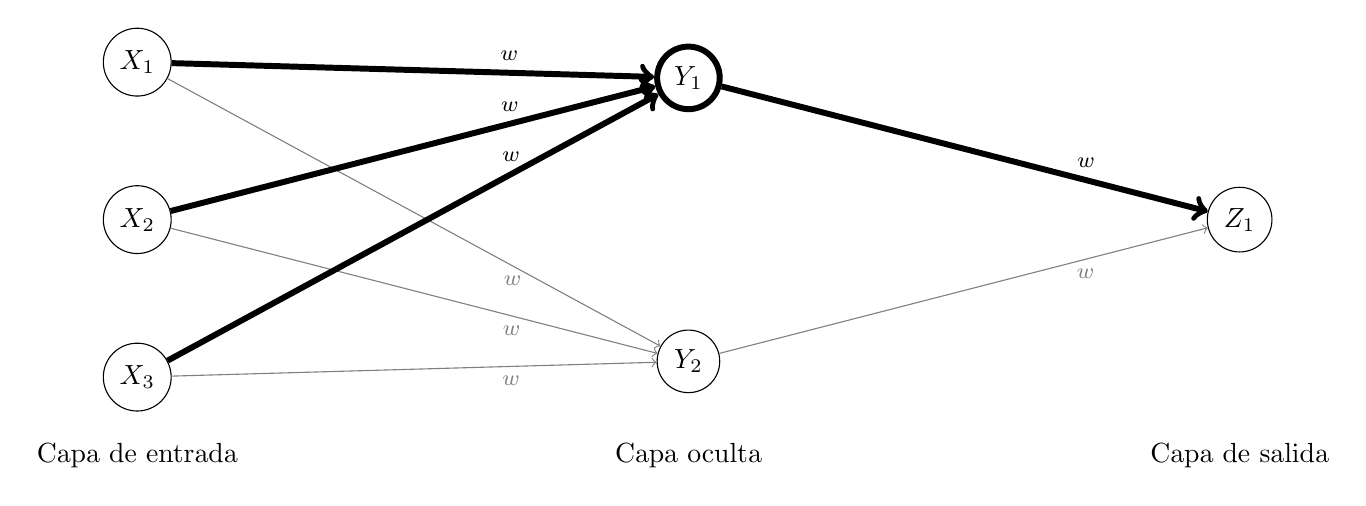
\begin{tikzpicture}

	\tikzstyle{nodo}=[circle, draw, minimum size=5ex]
	\tikzstyle{upw}=[dashed, red, ->, line width = 1pt]
	\tikzstyle{bold}=[line width=0.5ex]

	\coordinate (l_0) at (0, 3.5);
	\coordinate (l_1) at (7, 3.5);
	\coordinate (l_2) at (14, 3.5);
	\coordinate (input) at (0, -3.0);
	\coordinate (hidden) at (7, -3.0);
	\coordinate (output) at (14, -3.0);

	\coordinate (f_1_1) at (0, 2.0); % CAPA ENTRADA
	\coordinate (f_1_2) at (0, 0); % CAPA ENTRADA
	\coordinate (f_1_3) at (0, -2.0); % CAPA ENTRADA
	\coordinate (f_2_1) at (7, 1.8); % CAPA OCULTA 1
	\coordinate (f_2_2) at (7, -1.8); % CAPA OCULTA 1
	\coordinate (f_3_1) at (14, 0); % CAPA SALIDA

	%\node[] (l_0) at (l_0) {$L - 1$};
	%\node[] (l_1) at (l_1) {$L$};
	%\node[] (l_2) at (l_2) {$L + 1$};
	\node[] (input) at (input) {Capa de entrada};
	\node[] (hidden) at (hidden) {Capa oculta};
	\node[] (output) at (output) {Capa de salida};

	\node[nodo] (f_1_1) at (f_1_1) { $X_1$}; % CAPA ENTRADA
	\node[nodo] (f_1_2) at (f_1_2) { $X_2$}; % CAPA ENTRADA
	%\node[nodo] (f_1_3) at (f_1_3) {\Large $f_i(e_i)$}; % CAPA ENTRADA
	\node[nodo] (f_1_3) at (f_1_3) { $X_3$}; % CAPA ENTRADA
	\node[nodo, bold] (f_2_1) at (f_2_1) { $Y_1$}; % CAPA OCULTA 1
	\node[nodo] (f_2_2) at (f_2_2) { $Y_2$}; % CAPA OCULTA 1
	\node[nodo] (f_3_1) at (f_3_1) { $Z_1$}; % CAPA SALIDA


	\draw[->, font=\footnotesize, gray] (f_1_1) -- node[pos=0.70, below] (w_2_1) {$w$} (f_2_2);
	\draw[->, font=\footnotesize, gray] (f_1_2) -- node[pos=0.70, below] (w_2_2) {$w$} (f_2_2);
	\draw[->, font=\footnotesize, gray] (f_1_3) -- node[pos=0.70, below] (w_2_3) {$w$} (f_2_2);
	\draw[->, font=\footnotesize, bold] (f_1_1) --  node[pos=0.7, above] (w_1_1) {$w$} (f_2_1);
	\draw[->, font=\footnotesize, bold] (f_1_2) --  node[pos=0.70, above] (w_1_2) {$w$} (f_2_1);
	\draw[->, font=\footnotesize, bold] (f_1_3) -- node[pos=0.70, above] (w_1_3) {$w$} (f_2_1);

	\draw[->, font=\footnotesize, gray] (f_2_2) -- node[near end, below] {$w$} (f_3_1);
	\draw[->, font=\footnotesize, bold] (f_2_1) -- node[near end, above ] (w_j_k) {$w$} (f_3_1);
\end{tikzpicture}
}
	\caption{Esquema de una red neuronal}
	\label{fig:nn}
\end{imagen}

La activación de una neurona $Y$ está dado por su función de activación y las entradas. Alguna de las funciones de activación mas comunes se pueden ver en la tabla \ref{tab:f_activacion}. La entrada a la neurona $Y$ corresponde a la suma ponderada de los pesos de las conexiones que llegan hacia $Y$ por la salida de las neuronas de la capa anterior. En la figura \ref{fig:nn} se puede ver un modelo de tres capas, con una capa oculta. donde las salidas de las neuronas de la capa de entrada llegan hacia las neuronas $Y_1$ e $Y_2$ de la capa oculta para aplicar su función de activación respectiva, y sus salida son enviadas a la capa de salida.

\begin{table}[H]
	\centering
	\begin{tabular}{|l|c|c|}\hline
		{\bf Función}	& {\bf Fórmula}	& {\bf Rango}\\\hline
		Identidad & $f(x) = x$	& $[-\infty, \infty]$\\\hline
		Lineal por tramos &
		$f(x) = \left\{
		\begin{array}{ll}
			-1		& x < -1\\
			a*x		& -1 \leq x \leq 1\\
			1		& x > 1
		\end{array}
		\right. $	& $[-1, 1]$\\\hline
		Sinusoidal	& $ f(x) = \sin(\omega x + \varphi) $	& $[-1, 1]$\\\hline
		Sigmoidal	& $f(x) = \frac{1}{1 + \exp{-x}}$	& $[0, 1]$\\\hline
		Tangente hiperbólica	& $\frac{1 - \exp(-x)}{1 + \exp(-x)}$	& $[-1, 1]$\\\hline
	\end{tabular}
	\caption{Algunas funciones de activaciones.}
	\label{tab:f_activacion}
\end{table}

Las NN multicapa definen una relación entre la entrada y la salida. Esta relación se obtiene propagando hacia adelante los valores de las variables de entrada, es por esto que también se les llama redes {\em feedforward}. Cada neurona de la red procesa la entrada recibida y produce una respuesta que se propaga, mediante las conexiones, hacia las neuronas de la capa siguiente.

Existen dos fases importante dentro del modelo
\begin{itemize}
	\item Fase de entrenamiento: Se usa un conjunto de datos o patrones de entrenamiento para determinar los pesos que definen el modelo de la NN. Se calculan de manera iterativa, de acuerdo con los valores de entrenamiento, con el objeto de minimizar el error cometido entre la salida obtenida por la NN y la salida deseada.

	Los pesos óptimos se obtienen minimizando una función. Uno de los criterios utilizados es la minimización del error cuadrático medio entre el valor de salida y el valor real esperado.

	\item Fase de prueba: Durante el entrenamiento, el modelo se ajusta al conjunto de entrenamiento, perdiendo la habilidad de generalizar su aprendizaje a casos nuevos, a esta situación se le llama sobreajuste.

	Para evitar el sobreajuste, se utiliza un segundo grupo de datos diferentes, el conjunto de validación, que permitirá controlar el proceso de aprendizaje.
\end{itemize}


\subsection{El algoritmo de entrenamiento por retropropagación y el desvanecimiento del gradiente}
El algoritmo de retropropagación del error, también conocido como la regla delta, fue el primer algoritmo de entrenamiento para redes multicapas  \cite{Werbos1974, Rumelhart1986}. El término retropropagación es utilizado debido a la forma de implementar el método del gradiente en las redes multicapa, pues el error cometido en la salida de la red es propagado hacia atrás, transformándolo en un error para cada una de las neuronas ocultas de la red. El entrenamiento de una red por retropropagación implica tres etapas: la propagación del patrón de entrada, el cálculo del error y su propagación hacia las capas anteriores, y el ajuste de los pesos. Después del entrenamiento, la aplicación de la red implica solamente los cálculos de la fase de propagación. En caso de que el entrenamiento sea lento, una red ya entrenada puede producir su salida rápidamente.


El funcionamiento del agoritmo de retropropagación se puede apreciar en la figura \ref{fig:backprop}. Se representa en azul primera fase del algoritmo, donde la entrada de la red se propaga hacia la salida a través de las neuronas transformandola en cada neurona de la red. La segunda fase, en verde, muestra como se propaga, desde la salida, el error hacia las capas anteriores. Finalmente, se puede ver en rojo como el algoritmo actualiza los pesos de la red utilizando el error que genera la red.
\begin{imagen}
	\scalebox{1.0}{% http://staff.itee.uq.edu.au/janetw/cmc/chapters/BackProp/index2.html
% http://outlace.com/Beginner-Tutorial-Backpropagation/
% http://neuralnetworksanddeeplearning.com/chap2.html
% http://staff.itee.uq.edu.au/janetw/cmc/chapters/BackProp/slides/Backprop_files/frame.htm
% http://staff.itee.uq.edu.au/janetw/cmc/chapters/BackProp/
% http://home.agh.edu.pl/~vlsi/AI/backp_t_en/backprop.html
% https://www.google.cl/webhp?sourceid=chrome-instant&ion=1&espv=2&ie=UTF-8#safe=off&q=backpropagation+practice+example
% https://ayearofai.com/rohan-4-the-vanishing-gradient-problem-ec68f76ffb9b#.9ntv81akz

\ifx\du\undefined
  \newlength{\du}
\fi
\newcommand{\nweigth}[2]{$W^{#1}_{#2} - \alpha\frac{\partial J}{\partial W^{#1}_{#2}}$}
\newcommand{\w}[2]{$W^{#1}_{#2}$}

\setlength{\du}{1\unitlength}
\begin{tikzpicture}[font=\small]
\tikzstyle{neuron}=[circle,draw, minimum size=2em]
\tikzstyle{update}=[dashed, blue]

\pgftransformxscale{1.000000}
\pgftransformyscale{-1.000000}

\coordinate (x1)    at (0.000000\du, 0.000000\du);
\coordinate (x2)    at (0.000000\du, 8.000000\du);

\coordinate (i)     at (3.000000\du, 0.000000\du);
\coordinate (ii)    at (3.000000\du, 8.000000\du);

\coordinate (iv)    at (10.000000\du, 0.000000\du);
\coordinate (v)     at (10.000000\du, 8.000000\du);

\coordinate (vii)   at (17.000000\du, 0.000000\du);
\coordinate (viii)  at (17.000000\du, 8.000000\du);

\coordinate (ix)   at (17.000000\du, 0.000000\du);
\coordinate (diez)  at (17.000000\du, 8.000000\du);


\coordinate (x)     at (24.000000\du, 4.000000\du);
\coordinate (y)     at (27.000000\du, 4.000000\du);


%%%%%%%%%%%%%%%%%%%%%%%%%%%%%%%%%%%%%%%%%%%%%%%%%%%%%%%%%%
% ENTRADA
\node (X1) at (x1) {\Huge $x_1$};
\node (X2) at (x2) {\Huge $x_2$};

% CAPA DE ENTRADA
\node[neuron] (A) at  (i) {}; % A
\node[neuron] (B) at  (ii)  {}; % B

% CAPA 1
\node[neuron] (C) at  (iv)  {}; % C
\node[neuron] (D) at  (v)  {}; % D

% CAPA 2
\node[neuron] (E) at  (vii)  {}; % E
\node[neuron] (F) at  (viii)  {}; % F

% CAPA 2
\node[neuron] (H) at  (ix)  {}; % E
\node[neuron] (I) at  (diez)  {}; % F

% CAPA DE SALIDA
\node[neuron] (G) at  (x)  {}; % G

% SALIDA
\node (out) at (y) {\Huge $y_1$};
%%%%%%%%%%%%%%%%%%%%%%%%%%%%%%%%%%%%%%%%%%%%%%%%%%%%%%%%%%


\draw[->] (X1) -- (A);
\draw[->] (X2) -- (B);


%%%%%%%%%%%%%%%%%%%%%%%%%%%%%%%%%%%%%%%%%%%%%%%%%%%%%%%%%%
%%%%%%%%%%%%%%%%%%%%%%%%%%%%%%%%%%%%%%%%%%%%%%%%%%%%%%%%%%
\draw[->] (A) -- node[above, pos=0.2] (W_1_11) {\w{1}{11}} (C);
\draw[->] (A) -- node[left , pos=0.2] (W_1_12) {\w{1}{12}} (D);
\draw[->] (B) -- node[left , pos=0.2] (W_1_13) {\w{1}{13}} (C);
\draw[->] (B) -- node[below, pos=0.2] (W_1_14) {\w{1}{14}} (D);

%\draw[->, dashed, blue] (C) to [bend left=40] node[above] {$W^{1}_{11} - \alpha\frac{\partial J}{\partial W^{1}_{11}}$} (W_1_11);
\draw[->, update] (C) to [bend left=40] node[above] {\nweigth{1}{11}} (W_1_11);
\draw[->, update] (D) to [bend left=50] node[above right, pos=0.98] {\nweigth{1}{12}} (W_1_12);

\draw[->, update] (C) to [bend right=50] node[below right, pos=0.98] {\nweigth{1}{13}} (W_1_13);
\draw[->, update] (D) to [bend right=40] node[below] {\nweigth{1}{14}} (W_1_14);

%%%%%%%%%%%%%%%%%%%%%%%%%%%%%%%%%%%%%%%%%%%%%%%%%%%%%%%%%%
%%%%%%%%%%%%%%%%%%%%%%%%%%%%%%%%%%%%%%%%%%%%%%%%%%%%%%%%%%
\draw[->] (C) -- node[above, pos=0.2] (W_2_11) {\w{l}{11}} (E);
\draw[->] (C) -- node[left , pos=0.2] (W_2_12) {\w{2}{12}} (F);
\draw[->] (D) -- node[left , pos=0.2] (W_2_13) {\w{2}{13}} (E);
\draw[->] (D) -- node[below, pos=0.2] (W_2_14) {\w{2}{14}} (F);

\draw[->, update] (E) to [bend left=40] node[above] {\nweigth{2}{11}} (W_2_11);
\draw[->, update] (F) to [bend left=50] node[above right, pos=0.98] {\nweigth{2}{12}} (W_2_12);

\draw[->, update] (E) to [bend right=50] node[below right, pos=0.98] {\nweigth{2}{13}} (W_2_13);
\draw[->, update] (F) to [bend right=40] node[below] {\nweigth{2}{14}} (W_2_14);

%%%%%%%%%%%%%%%%%%%%%%%%%%%%%%%%%%%%%%%%%%%%%%%%%%%%%%%%%%
%%%%%%%%%%%%%%%%%%%%%%%%%%%%%%%%%%%%%%%%%%%%%%%%%%%%%%%%%%
\draw[->] (E) -- node[right, pos=0.2] (W_3_11) {\w{3}{11}} (G);
\draw[->] (F) -- node[right, pos=0.2] (W_3_12) {\w{3}{12}} (G);

\draw[->, update] (G) to [bend  left=50] node[above right, pos=0.98] {\nweigth{3}{11}} (W_3_11);
\draw[->, update] (G) to [bend right=40] node[below right, pos=0.98] {\nweigth{3}{12}} (W_3_12);


\draw[->] (G) -- (out);
\end{tikzpicture}
}
	\caption{Esquema del algoritmo de retropropagación.}
	\label{fig:backprop}
\end{imagen}

Si un perceptrón multicapa con $C$ capas y $n_c$ neuronas en la capa $c$, donde $W_c = (w^{c}_{ij})$ es la matriz de pesos, $w^{c}_{ij}$ representará el peso de la conexion de la neurona $i$ de la capa $c$ hasta la neurona $j$ de la capa siguiente. Denotaremos $a^{c}_{i}$ a la activación de la neurona $i$ de la capa $c$ que se calcula de la siguiente manera:
\begin{itemize}
	\item {\bf Activación de una neurona de la capa de entrada}: Las neuronas se encargan de transmitir la entrada recibida, por lo tanto $$ a^{1}_{i} = x_{i}, i = 1, 2, \cdots, n$$ donde $X = (x_1, x_2, \cdots, x_n)$ representa el vector de entrada.

	\item {\bf Activación de una neurona de la capa oculta}: Las neuronas de una capa oculta procesa la información recibida aplicando la función $f$ a la suma de los productos de la entrada por sus pesos, es decir $$ a^{c}_{i} = f\left(\sum^{n_{c - 1}}_{j=1} w^{c - 1}_{ji}a^{c - 1}_{j} + \theta^{c}_{i}\right), i = 1, 2, \cdots, n_c; c = 2, 3, \cdots, C - 1$$ donde $a^{c - 1}_{j}$ es la salida de la capa anterior a $c$.

	\item {\bf Activación de una neurona de la capa de salida}: La activación de una neurona de la capa de salida viene dada por la función $f$ aplicada a la suma de los productos de la entrada por sus pesos, es decir $$ y_{i} = a^{c}_{i} = f\left(\sum^{n_{c - 1}}_{j=1} w^{C - 1}_{ji}a^{C - 1}_{j} + \theta^{C}_{i}\right), i = 1, \cdots, n_c$$ donde $Y = (y_1, y_2, \cdots, y_{n_{c}})$ es el vector de salida.
\end{itemize}

La función $f$ es la función de activación de la neurona. Aunque existe gran variedad de funciones de activación (ver tabla \ref{tab:f_activacion}), las funciones de activación mas utilizadas son la sigmoidal y la tangente hiperbólica, descritas en las escuaciones \ref{eq:sigm} y \ref{eq:tanh} respectivamente.
\begin{eqnarray}
	f_{sigm}(x) &=& \frac{1}{1+\exp(-x)}\label{eq:sigm}\\
	f_{tanh}(x) &=& \frac{1 - \exp(-x)}{1 + \exp(-x)}\label{eq:tanh}
\end{eqnarray}

Ambas funciones poseen como imagen un intervalo de valores entre $[0, 1]$ y $[-1, 1]$ como se observa en la figura \ref{fig:funciones}.% y están descritas por las ecuaciones \ref{eq:sigm} y \ref{eq:tanh}.

\begin{imagen}
	\scalebox{1.0}{
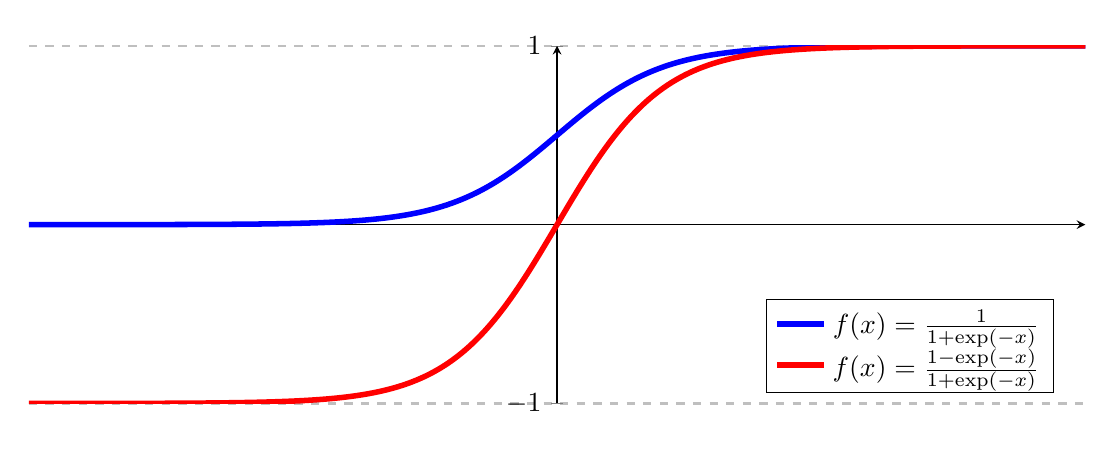
\begin{tikzpicture}
\begin{axis}[ymin=-1, ymax = 1, axis lines = left, legend pos=south east, width=15cm, xmajorticks=false, ytick={-1, +1}, axis lines=middle, y post scale=0.4, ymajorgrids=true, major grid style={dashed, line width=0.8pt}, yticklabel pos=left]
%Here the blue parabloa is defined
\addplot[domain=-10:10, samples=1000, color=blue, line width=2pt]{1/(1 + exp(-x))};
\addplot[domain=-10:10, samples=1000, color=red, line width=2pt]{(1 - e^(-x))/(1 + e^(-x))};
\addlegendentry{$f(x) = \frac{1}{1+\exp(-x)}$}
\addlegendentry{$f(x) = \frac{1 - \exp(-x)}{1 + \exp(-x)}$}
\end{axis}
%\begin{axis}[ymin=-1, ymax = 1, axis lines = left, xlabel = $x$, ylabel = {$f(x)$}]
%%Here the blue parabloa is defined
%\addplot[domain=-10:10, samples=1000, color=red]{(1 - e^(-x))/(1 + e^(-x))};
%\addlegendentry{$(1 - \exp(-x))/(1 + \exp(-x))$}
%\end{axis}
\end{tikzpicture}
% 1/(1+exp(-x))
}
	\caption{Funciones de activación mas utilizadas.}
	\label{fig:funciones}
\end{imagen}

Las NN multicapa actualizan sus pesos en función de una regla de aprendizaje, de tal manera que los nuevos pesos permitan reducir el error de salida. Por tanto, para cada patrón de entrada necesario disponer de una de salida deseada. El objetivo es que la salida de la red sea lo más próxima posible a la salida deseada, debido a esto es que el aprendizaje de la red se describe como un problema de minimización de la siguiente manera $$ \min_{W} E $$ donde $W$ es el conjunto de parámetros de la red (pesos y umbrales) y $E$ es una función de error que evalúa la diferencia entre las salidas de la red y las salidas deseadas. En la mayor parte de los casos, la función de error se define como:
\begin{eqnarray}
	E = \frac{1}{N}\sum^{N}_{i = 1} e(i)
\end{eqnarray}

Donde $N$ es el número de muestras y $e(n)$ es el error cometido por la red para el patrón $i$, definido de la siguiente manera
\begin{eqnarray}
	e(i) = \frac{1}{n_{C}}\sum^{n_{C}}_{j = 1} (s_{j}(i) - y^{j}(n))^2\label{eq:error_patron}
\end{eqnarray}

Siendo $Y(i) = (y_{1}(i), y_{2}(i), \cdots, y_{n_{C}}(i))$ y $S(i) = (s_{1}(i), s_{2}(i), \cdots, s_{n_{C}}(i))$ los vectores de salida y salidas deseadas para el patrón $i$ respectivamente.

De esta manera, si $W^{*}$ es un mínimo de la función de error $E$, en dicho punto el error será cercano a cero, y en consecuencia, la salida de la red será próxima a la salida deseada. La presencia de funciones de activación no lineales hace que la respuesta de la red sea no lineal respecto a los parámetros ajustables, por lo que el problema de minimización es un problema no lineal y se hace necesario el uso de técnicas de optimización no lineales para su resolución.

Las técnicas de actualización utilizadas suelen basarse en la actualización de los parámetros de la red mediante la determinación de una dirección de búsqueda. En el caso de las NN multicapa, la dirección de búsqueda más utilizada se basa en la dirección contraria del gradiente de la función de error $E$, el método de gradiente descendente. El procedimiento está basado en una sucesión de minimizaciones del error $e(i)$ por cada patrón, en lugar de minimizar el error total $E$ de la red. Aplicando el método cada parámetro $w$ se modifica según la siguiente regla de aprendizaje
\begin{eqnarray}
	w(i) = w(i - 1) - \alpha\frac{\partial e(i)}{\partial w}\label{eq:update}
\end{eqnarray}
donde $e(i)$ es el error para el patrón de entrada $i$ dado por la ecuación \ref{eq:error_patron}, y $\alpha$ es la tasa de aprendizaje, éste último determina el desplazamiento en la superficie del error.

%%%%%%%%%%%%%%%%%%%%%%%%%%%%%%%%%%%%%%%%%%%%%%
%%%%%%%%%%%%%%%%%%%%%%%%%%%%%%%%%%%%%%%%%%%%%%
% DESVANECIMIENTO DEL GRADIENTE
A medida que el error se propaga a través de la red, los pesos se actualizarán según la ecuación \ref{eq:update}, utilizando funciones cuyo gradiente se encuentra entre 0 y 1. Debido a que estos gradientes se multiplican durante la retropropagación, tienden a {\em desvanecerse} a través de las capas, y en una NN profunda esto evita que los pesos de las primeras capas ocultas se actualicen minimamente.

Si se tiene una NN, la activación de una neurona de una capa intermedia $i$ con función de activación $f$ es $y^{i}(t) =  f_{i}(net_{i}(t))$ donde $$ net_{i}(t) = \sum_{j}w_{ji}y^{j}(t - 1) $$ es la entrada a la neurona. Además $w_{ji}$ es el peso de la conexión desde la unidad $j$ de la capa anterior hasta la unidad $i$ de la capa actual, $d_{k}(t)$ será la respuesta esperada de la unidad $k$ de la capa de salida en el tiempo $t$. Usando el error cuadrático medio ({\em Mean square error}, MSE), el error de $k$ será
$$ E_{k}(t) = (d_{k}(t) - y^{k}(t))^2 $$



%Si se tiene una NN, la activación de una neurona de una capa intermedia $i$ con función de activación $f_i$ y con entrada $$ net_{i}(t) = \sum_{j}w_{ji}y^{j}(t - 1) $$ es $$y^{i}(t) = f_{i}(net_{i}(t))$$ Además $w_{ji}$ es el peso de la conexión desde la unidad $j$ de la capa anterior hasta la unidad $i$ de la capa actual, $d_{k}(t)$ será la respuesta esperada de la unidad $k$ de la capa de salida en el tiempo $t$. Usando el error cuadrático medio ({\em Mean square error}, MSE), el error de $k$ será $$ E_{k}(t) = (d_{k}(t) - y^{k}(t))^2 $$

En un tiempo $\tau \leq t$ cualquiera, el error de una neurona $j$ que no sea una neurona de entrada es la suma de los errores externos y el error propagado hacia atrás desde la neurona previa será
$$ \vartheta_{j}(\tau) = f'_{j}(net_{j}(\tau))\left(E_{j}(\tau) + \sum_{i} w_{ij}\vartheta_{i}(\tau + 1)\right) $$

El peso actualizado en el tiempo $\tau$ resulta $w_{jl}^{new} = w_{jl}^{old} + \alpha\vartheta_{j}(\tau) y^{l}(\tau - 1)$ donde $\alpha$ es la tasa de aprendizaje, y $l$ es una unidad arbitraria conectada a la unidad $j$.

%\citeA{Puskorius1994}
La propagación hacia atrás de un error que ocurre en una unidad $u$ en un tiempo $t$ hacia una unidad $v$ para $q$ pasos, escala el error de la siguiente manera
\begin{eqnarray}
\frac{\partial\vartheta_{v}(t - q)}{\partial\vartheta_{u}(t)} =
\left\{
\begin{array}{lr}
	f^{'}_{v}(net_{v}(t - 1))w_{uv}	& q = 1\\
	\\
	f^{'}_{v}(net_{v}(t - q))\sum^{n}_{l=1}\frac{\partial\vartheta(t - q + 1)}{\partial\vartheta_{u}(t)}w_{lv}	& q > 1
\end{array}
\right.
\end{eqnarray}

Con $l_{q} = v$ y $l_{0} = u$, el factor de escalamiento es
\begin{eqnarray}
\frac{\partial\vartheta_{v}(t - q)}{\partial\vartheta_{u}(t)} =
\sum^{n}_{l_{1}=1}\cdots\sum^{n}_{l_{q - 1}=1}\prod^{q}_{m = 1}f^{'}_{l_{m}}(net_{l_{m}}(t - m))w_{l_{m}l_{m - 1}}\label{eq:vanishing}
\end{eqnarray}

La sumatoria de los $n^{q - 1}$ términos $\prod^{q}_{m = 1}f^{'}_{l_{m}}(net_{l_{m}}(t - m))w_{l_{m}l_{m - 1}}$ escalan el error. Los distintos términos pueden tener signos diferentes, por lo tanto, el aumento del número de unidades $n$ no implica un incremento del error absoluto. Pero con mas unidades se incrementa la expectativa de que el valor absoluto del error aumente. Si $\rho(m, l_{m}, l_{m - 1}) := |f^{'}_{l_{m}}(net_{l_{m}}(t - m))w_{l_{m}l_{m - 1}}| < 1.0$
para todo $m$, el producto en (\ref{eq:vanishing}) decrece exponencialmente con $q$, es decir, el error se desvanece como muestra la figura \ref{fig:vanishing}. Un error que se desvanece a lo largo del flujo casi no tiene efecto en la actualización de los pesos. %Dada la constante $y^{l_{m - 1}} \neq 0$, $\rho(m, l_{m}, l_{m - 1})$ es máximo cuanto $w_{l_{m}l_{m - 1}} = \frac{1}{y^{l_{m - 1}}}\coth(\frac{net_{l_{m}}}{2})$.

\begin{imagen}
	\scalebox{1.0}{\begin{tikzpicture}

	\tikzstyle{nodo}=[circle, draw, minimum size=1.25cm]
	\tikzstyle{upw}=[dashed, red, ->, line width = 1pt]
	\tikzstyle{cnx}=[->, decoration={markings,mark=at position 1 with {\arrow[scale=2]{>}}}, postaction={decorate},]

	\coordinate (l_0) at (0.0, 5.5);
	\coordinate (l_1) at (6.0, 5.5);
	\coordinate (l_2) at (12, 5.5);

	\coordinate (f_1_1) at (0, 3.5); % CAPA ENTRADA
	\coordinate (f_1_2) at (0, 0); % CAPA ENTRADA
	\coordinate (f_1_3) at (0, -3.5); % CAPA ENTRADA
	\coordinate (f_2_1) at (6.0, 2.7); % CAPA OCULTA 1
	\coordinate (f_2_2) at (6.0, -2.7); % CAPA OCULTA 1
	\coordinate (f_3_1) at (12, 0); % CAPA SALIDA
	\coordinate (y) at (14, 0); % CAPA SALIDA

	\node[] (l_0) at (l_0) {$L - 1$};
	\node[] (l_1) at (l_1) {$L$};
	\node[] (l_2) at (l_2) {$L + 1$};

	\node[nodo, font=\small] (f_1_1) at (f_1_1) {$f_i(e_i)$}; % CAPA ENTRADA
	\node[nodo] (f_1_2) at (f_1_2) {}; % CAPA ENTRADA
	\node[nodo] (f_1_3) at (f_1_3) {}; % CAPA ENTRADA
	\node[nodo, font=\small] (f_2_1) at (f_2_1) {$f_j(e_j)$}; % CAPA OCULTA 1
	\node[nodo] (f_2_2) at (f_2_2) {}; % CAPA OCULTA 1
	\node[nodo] (f_3_1) at (f_3_1) {$f_k(e_k)$}; % CAPA SALIDA
	\node[] (y) at (y) {$y$}; % CAPA SALIDA

	\node[left of=f_1_1, node distance=1.4cm] {\LARGE $\cdots$};
	\node[left of=f_1_2, node distance=1.4cm] {\LARGE $\cdots$};
	\node[left of=f_1_3, node distance=1.4cm] {\LARGE $\cdots$};

	\draw[cnx] (f_1_1) -- node[pos=0.65, above] (w_1_1) {$w$} (f_2_1);
	\draw[cnx] (f_1_2) -- node[pos=0.65, above] (w_1_2) {} (f_2_1);
	\draw[cnx] (f_1_3) -- node[pos=0.65, above] (w_1_3) {} (f_2_1);
	\draw[cnx] (f_1_1) -- node[pos=0.65, below] (w_2_1) {$w$} (f_2_2);
	\draw[cnx] (f_1_2) node[below right of=f_1_2] {} -- node[pos=0.6, below] (w_2_2) {} (f_2_2);
	\draw[cnx] (f_1_3) -- node[pos=0.6, below] (w_2_3) {} (f_2_2);
	\draw[cnx] (f_2_1) node[left of=f_2_1] {} -- node[pos=0.5, above right] (w_j_k) {$w$} (f_3_1);
	\draw[cnx] (f_2_2) -- node[pos=0.5, below right] {} (f_3_1);
	\draw[cnx] (f_3_1) -- node[pos=0.5, below right] {} (y);

	\node[above right of=f_2_1, node distance=1.3cm, font=\scriptsize] {$e_{j} = \sum w_{ij}a_i$};



	\node[blue, above=0.2cm of f_3_1] (e_i) {$\delta^{l+1}_{k}$};
	\node[blue, right of=f_2_1] (e_2_1_i) {$\delta^{l}_{j}$};
	\node[blue, right of=f_2_2] (e_2_2_i) {$\delta^{l}$};
	\node[blue, above right=0.3cm and -1.0cm of f_1_1] (e_1_2_i) {$\delta^{l-1} = f^{'}_{i}(a_i)\sum_{j}w^{l-1}_{ij}\left(f^{'}_{j}(a_{j})\sum_{k}w^{l}_{jk}\delta^{l+1}_{k}\right)$};
	%\node[blue, above right=0.3cm and 0.0cm of f_1_1] (e_1_2_i) {$\delta^{l-1} = f'(a_i)\sum_{j}w^{l-1}_{ij}\delta^{l}_{j}$};

	\draw[upw, blue] (y) to[bend right=40] node[right]{$f'(y)$} (e_i);
	\draw[upw, blue] (f_3_1) to[bend right=10] node[above right, pos=0.7]{$f^{'}_{j}(a_{j})\sum_{k}w^{l}_{jk}\delta^{l+1}_{k}$} (e_2_1_i);
	%\draw[upw, blue] (f_3_1) to[bend left=10] (e_2_2_i);

	\draw[upw, blue] (f_2_1) to[bend right=5] (e_1_2_i);
	\draw[upw, blue] (f_2_2) to[bend right=5] (e_1_2_i);

\end{tikzpicture}
}
	\caption{Gradiente descendente}
	\label{fig:vanishing}
\end{imagen}
%%%%%%%%%%%%%%%%%%%%%%%%%%%%%%%%%%%%%%%%%%%%%%
%%%%%%%%%%%%%%%%%%%%%%%%%%%%%%%%%%%%%%%%%%%%%%


\section{Revisión de la literatura}
\subsection{El gradiente estocástico descendente}
\subsection{Retropropagación resiliente y RMSProp}
%\subsection{Retropropagación resiliente}
En las capas ocultas de las NN se utilizan con frecuencia funciones de activación sigmoidales, y estas reducen la entrada a un rango finito de salida. Se caracterizan por sus pendientes próximas a cero para entradas muy grandes, y esto representa un problema cuando se utiliza el gradiente descendente para el entrenamiento, pues se acentúa el problema del desvanecimiento del gradiente.

\citeA{Riedmiller1993} presenta el algoritmo de retropropagación resiliente ({\em Resilient retropropagation}, RPROP), con el que busca eliminar los efectos del desvanecimiento del gradiente, esto mediante el uso del signo de la derivada para determinar la dirección del ajuste de los pesos, haciendo que la magnitud de la derivada no tenga efecto sobre la actualización de los pesos de la NN. Los pesos de la NN se incrementarán por un factor $\Delta{i}$ cuando la derivada de la función respecto a dicho peso tenga el mismo signo que las dos iteraciones anteriores. Mientras que si la derivada de la función respecto a dicho peso cambia de signo respecto de la iteración anterior los pesos se decrementarán por un factor $\Delta_{d}$. En caso de que la derivada de la función respecto de dicho peso sea igual a cero, el valor de actualización no varía.

%\subsubsection{Root Mean Square RPROP}
\citeA{Tieleman2012} presentan el algoritmo de la raíz cuadratica media de retropropagación resiliente ({\em Root mean square resilient retropropagation}, RMSPROP), una variante  del algoritmo RPROP. Se propone mantener una media móvil del cuadrado del gradiente para cada peso
\begin{eqnarray}
	MeanSquare(w, t) &=& 0.9MeanSquare(w, t - 1) + 0.1\frac{\partial E}{\partial w^{(t)}}^{2}
\end{eqnarray}

Y dividiendo el gradiente por $\sqrt{MeanSquare(w, t)}$ hace que el aprendizaje funcione de mejor manera.


\subsection{Heurísticas y meta-heurísticas}
Hoy en día, resolver problemas computacionalmente complejos precisa el desarrollo de algoritmos más avanzados. Los algoritmos exactos a menudo utilizan una gran cantidad de tiempo debido al tamaño del espacio de soluciones factibles. Para resolver este inconveniente, se han diseñado algoritmos aproximados basados en el uso de heurísticas y meta-heurísticas, los que permiten encontrar soluciones que se aproximan a la mejor solución. Estos algoritmos utilizan funciones que están diseñadas para encontrar el espacio de soluciones de forma inteligente.

La figura \ref{fig:tax_opt} muestra la clasificación de diferentes problemas de optimización, los que se categorizan en: algoritmos exactos y algoritmos aproximados \cite{Desale2015}
%En la Figura \ref{fig:tax_opt} se muestra la clasificación de diferentes problemas de optimización, los cuales están divididos en dos categorías: algoritmos exactos y algoritmos aproximados \cite{Desale2015}.
\begin{figure}[H]
    \centering
    \includegraphics[scale=0.2]{img/tax_opt.png}
    \caption{Métodos para resolver problemas de optimización \protect\cite{Desale2015}.}
		\label{fig:tax_opt}
\end{figure}

Los algoritmos meta-heurísticos son un proceso iterativo que guía una heurística para explorar el espacio de búsqueda. Estos tipos de algoritmos son utilizados para encontrar una solución en un espacio de búsqueda discreto en problemas de optimización combinatoria.

%Las heurísticas y meta-heurísticas son utilizadas para encontrar una solución óptima en un espacio de búsqueda discreto en problemas de optimización combinatoria. Un ejemplo es el problema del vendedor viajero, donde la búsqueda del espacio de soluciones factibles crece exponencialmente en función del tamaño del problema aumenta, lo que hace inviable la realización de una búsqueda exhaustiva de la solución óptima \cite{Desale2015}.




\subsection{Simulated Annealing}
\subsection{Instancias}
